\chapter{Improvement Design, Implementation and Evaluation}%
\label{ch:improvement_design_implementation_and_evaluation}

% the idea: split the current empty Discussion chapter

This chapter covers the design, implementation and evaluation of an new development product of the CloudSentinel framework.

\section{Selected improvement and objectives}

Based on the evaluation of the base CloudSentinel framework, the following components have been designed:

\begin{itemize}
    \item 'Data Catalogue' for managing input datasets
    \item Model Importing and Training
    \item Anomaly Detection Model Comparisons
    \item Data Provenance
    \item Revised Live Monitoring
    % \item RCA generisability
\end{itemize}

\section{Design}
Broadly speaking, the design of what will be added and changed to the newly revised CloudSentinel framework can be put in four categories, starting with the 'Data Catalogue' component. This chapter covers each of these categories.

\subsection{Data Catalogue}
The evaluation concluded that data gathering in particular is one difficult part of CloudSentinel, as was also pointed out in the CloudSentinel evaluation of Van Gaalen (2024). CloudSentinel does not offer any mechanism that operators can use to gather a metrics dataset for the model-training. As a consequence, operators are forced to use their own roudabout mechanisms, such as custom scripts, to pull prometheus data  themselves, as well as put them in the right feature-column format and scale their values accordingly, such that they can be interpreted correctly by the anomaly detection algorithm in training. Furthermore, there is no data provenance present; meaning that once a model has been trained, the dataset that was used is not recorded and cannot be analysed at a later point.\\

In order to address these issues, we introduce a 'data catalogue' component. The data catalogue lets operators define and store dataset configurations as persistent objects, fetch the corresponding datawindows from Prometheus, and reuse these as many times as desired in different parts of the applications. It is intended to transform dataset management from tedious manual work into a task completed with a few button clicks.\\

In addition to descriptive metadata such as a dataset name and description, operators can assign a 'context workload' to each dataset. This categorises the dataset according to relevant workload characteristics, such as high or low CPU load. Although this information is not strictly required for model training, it is useful in that it helps operators distinguish between datasets and assess which types of workloads detector models identify effectively- and where their performance is limited.\\

The following figures give a low-fi overview of the user interface of the data catalogue component. Figure \ref{fig:data_cat_overview} displays the overview screen where users are able to view an overview of all the saved datasets. Figure \ref{fig:data_cat_add_dataset}  shows the 'add dataset' screen where users can define a new dataset. Figure \ref{fig:data_cat_view_dataset} displays the 'view dataset' screen, where users can view a saved dataset in detail.

\begin{figure}[H]
    \centering
    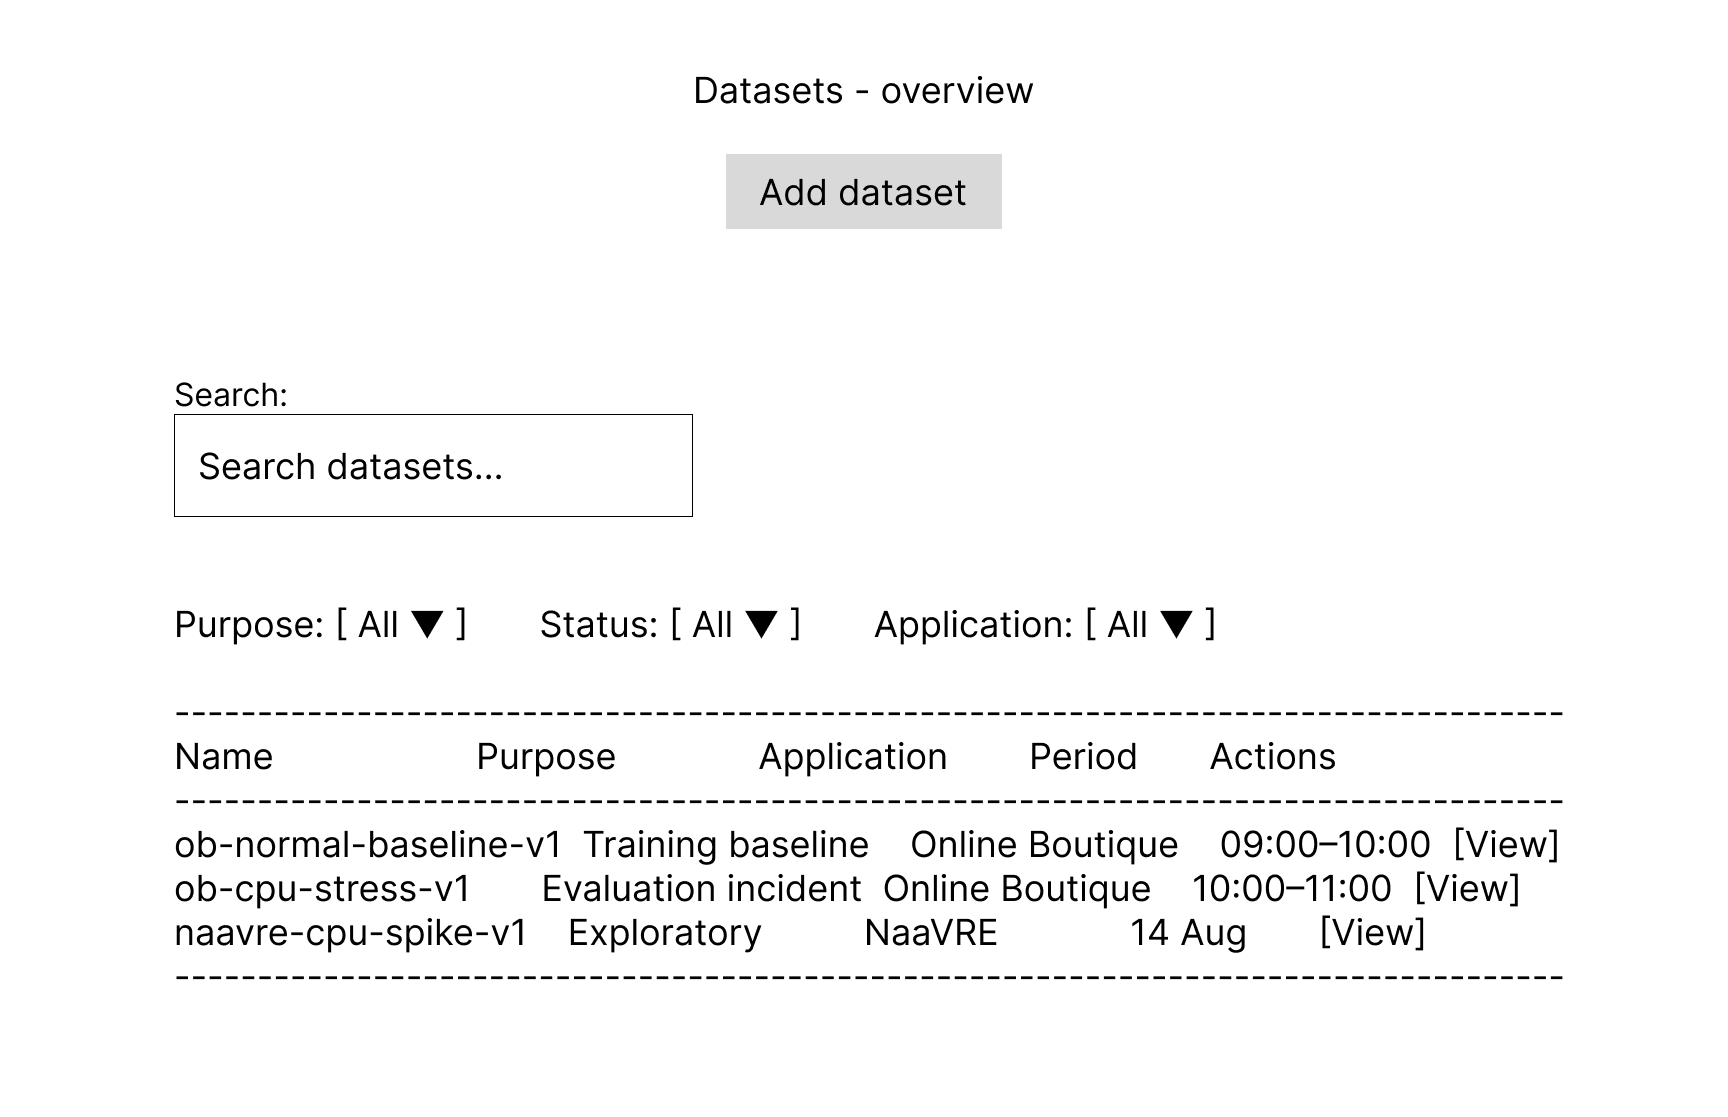
\includegraphics[width=1\linewidth]{figures/design/data_catalogue/Data Catalogue - overview.png}
    \caption{Data Catalogue: Overview}
    \label{fig:data_cat_overview}
\end{figure}

\begin{figure}[H]
    \centering
    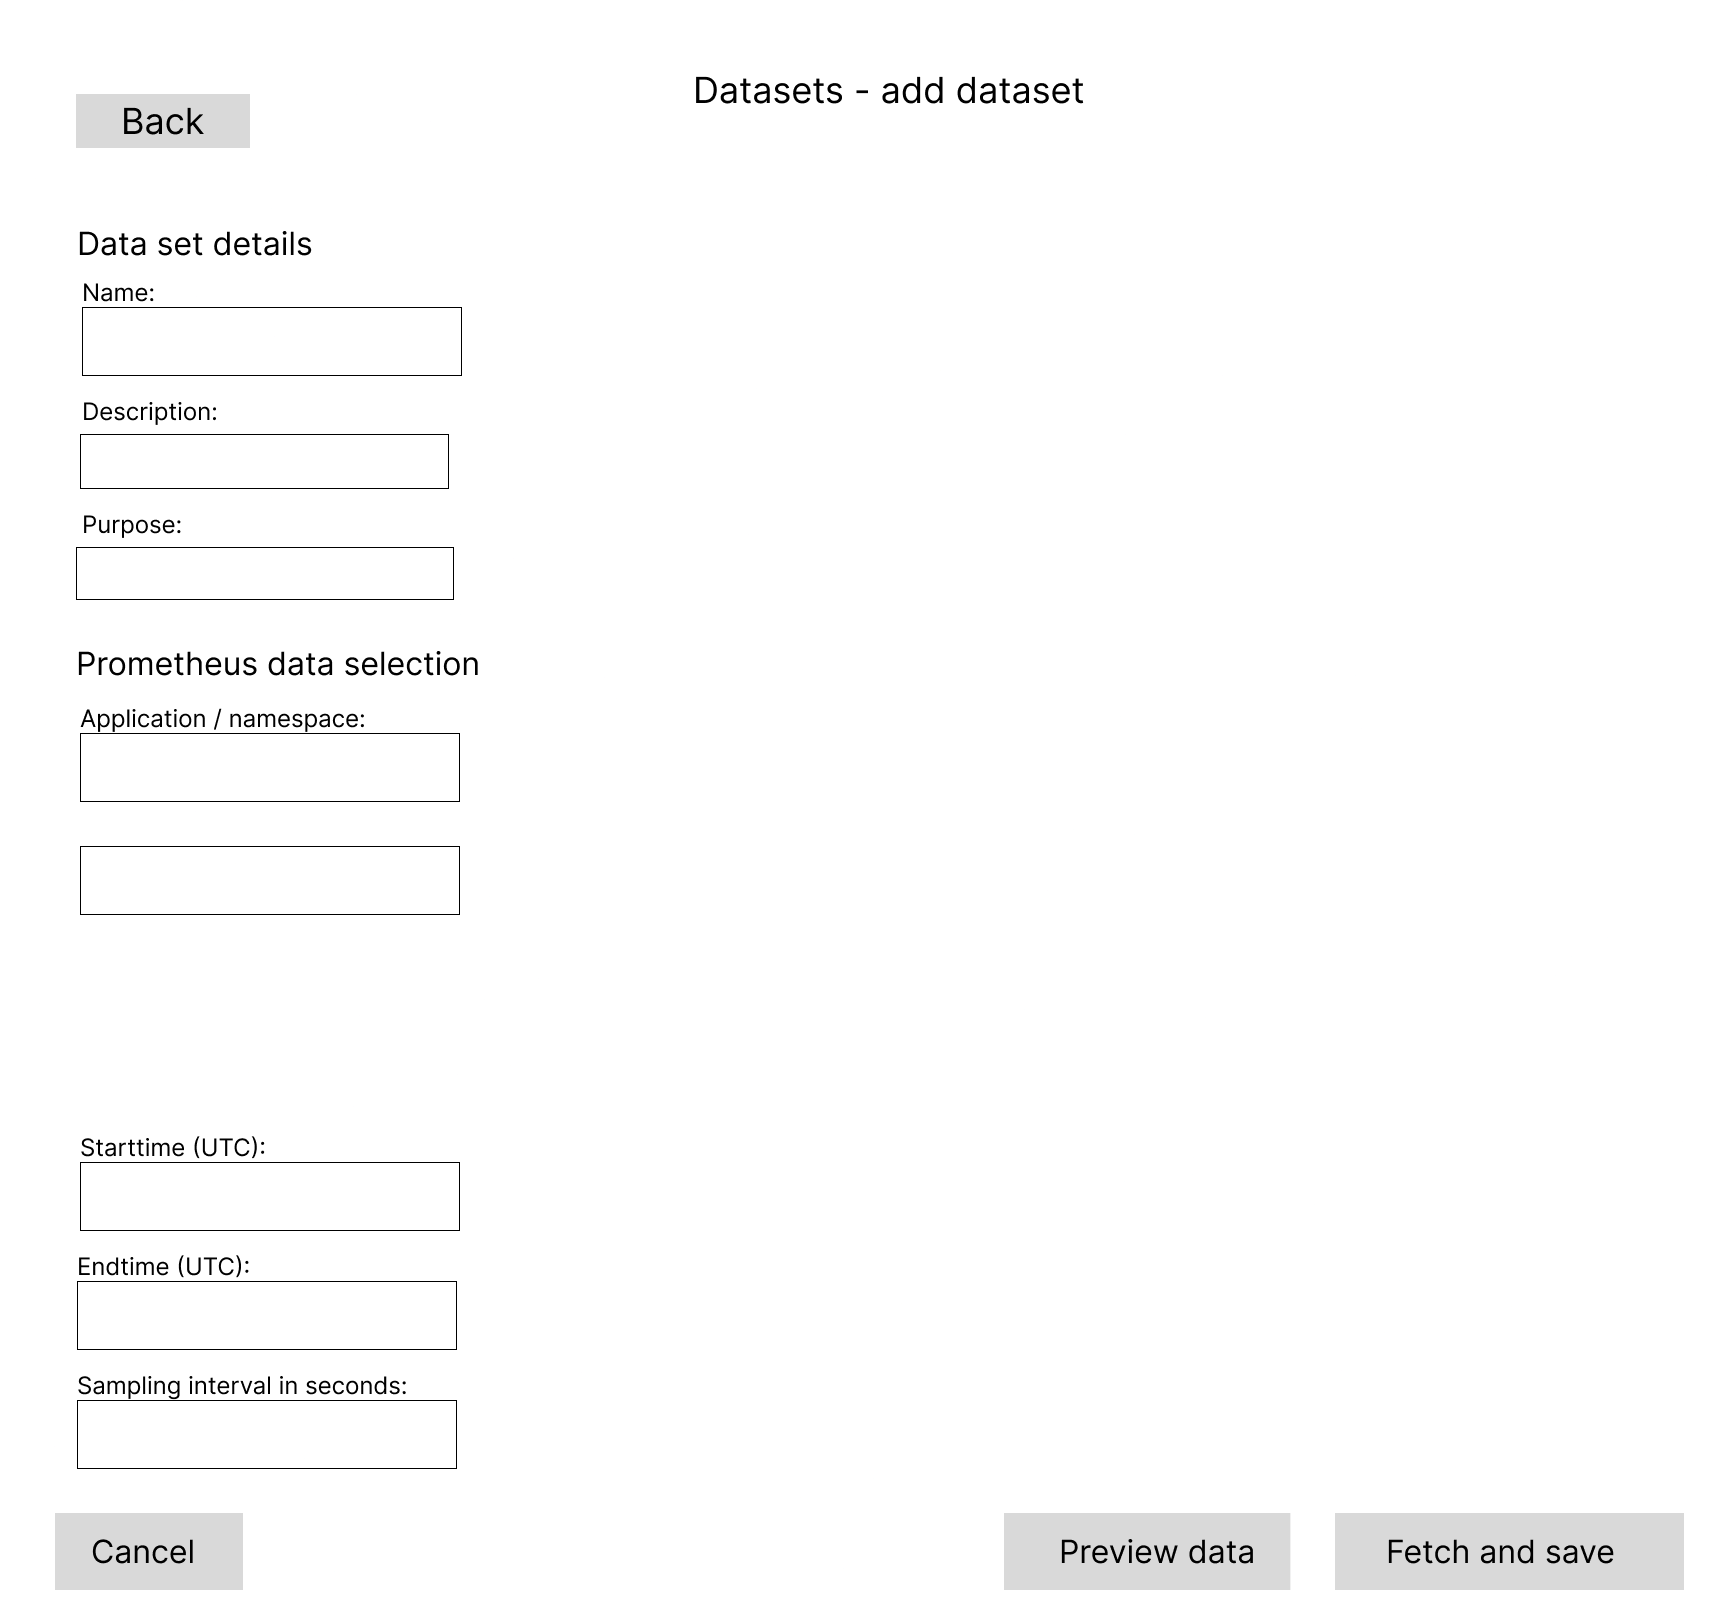
\includegraphics[width=1\linewidth]{figures/design/data_catalogue/Data Catalogue - add dataset.png}
    \caption{Data Catalogue: Add dataset}
    \label{fig:data_cat_add_dataset}
\end{figure}

\begin{figure}[H]
    \centering
    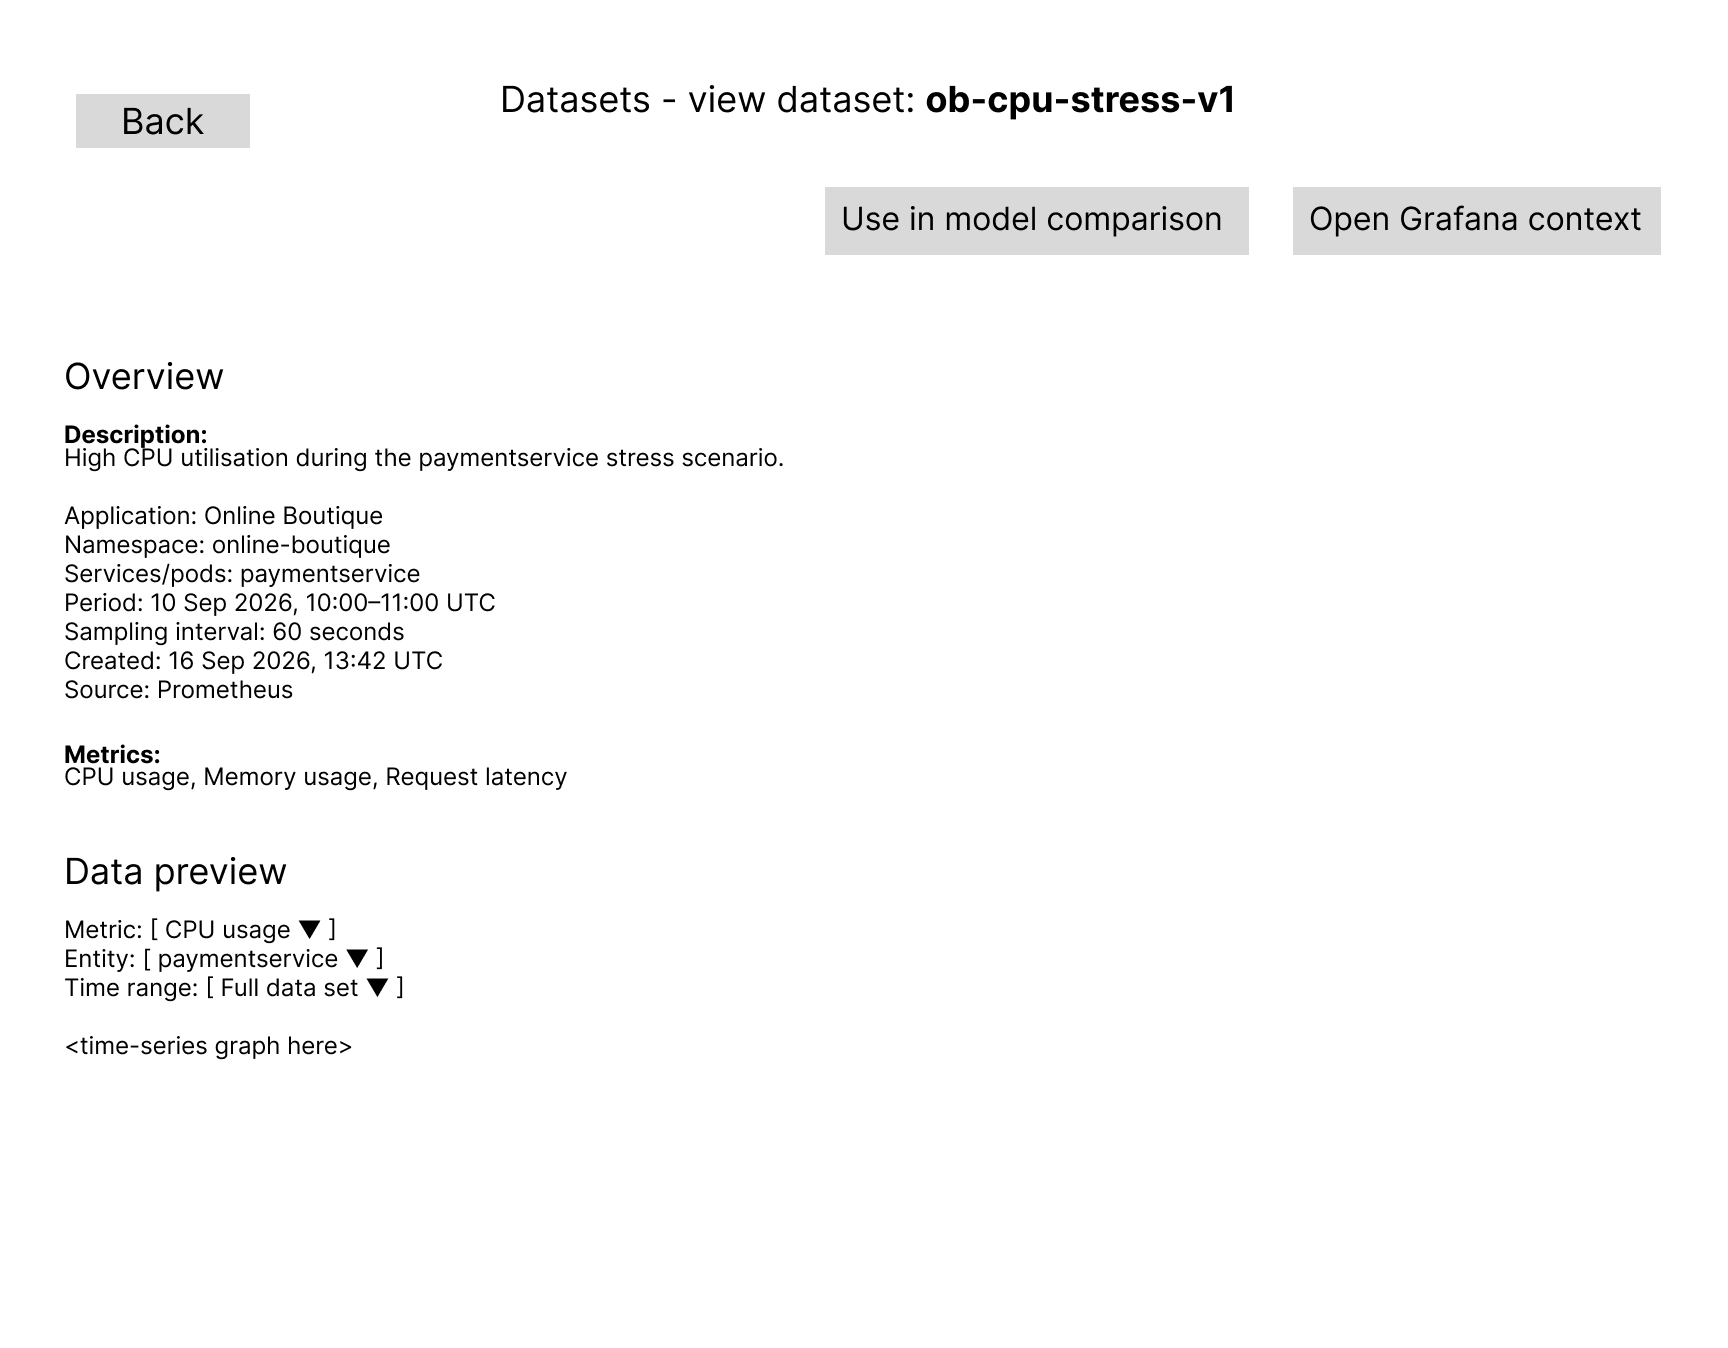
\includegraphics[width=1\linewidth]{figures/design/data_catalogue/Data Catalogue - view dataset.png}
    \caption{Data Catalogue: View Dataset}
    \label{fig:data_cat_view_dataset}
\end{figure}

\subsection{Managing Model Detectors and Training Pipeline}
In its current form, CloudSentinel is limited to the CGNN anomaly detection algorithm. However, under realistic circumstances, a framework like CloudSentinels would provide operators to have access to an algorithm of their own choosing rather than be forced to resort a single hardcoded detection algorithm. As such, the revised version of CloudSentinel is designed to incorporate functionality for adding custom detection algorithms. To incorporate this functionality, a custom adapter interface will be developed that operators can use to attach their own algorithm-implementations to. Ideally, an operator could develop and then 'drop' his algorithm implementation in a folder, where it will be discovered by CloudSentinel for later use.

The figures below display a low-fi design of the user interface layout. Figure \ref{fig:trained_models_overview} provides an entry point for inspecting the detector models available in the framework. Rather than treating a trained model as an isolated file, the design presents it as a managed artefact with identifiable metadata and a clear relationship to the detector implementation from which it was produced. The intent is to support data provenance in that operators are able to determine which model is available for use and subsequently inspect the configuration and training data associated with it.\\

Figure \ref{fig:register_detector_model} displays the workflow for registering an anomaly-detection algorithm. The interface is intended to make detector implementations discoverable and selectable without requiring changes to other parts of CloudSentinel. A registered detector can later be used in the training and comparison workflows. This design addresses the limitation of the baseline framework, which was restricted to a single hard-coded CGNN detector and did not demonstrate a clear mechanism for replacing or extending analytics components.\\

Figure \ref{fig:view_detector_details} displays the detector-details view, which provides the information required to understand the capabilities and requirements of a registered detector before it is used. More specifically: it gives operators a place to inspect the detector’s identity, implementation details, and supported configuration options. Some important information it provides are the data modality of the model (i.e. whether it supports metrics, logs or traces) as well as the  format of the expected input data, which as a default is expected to be Multivariate time series data. Generally, different anomaly-detection approaches may have different input requirements, parameters, and output semantics. The view therefore also helps separate detector-specific concerns from the broader dataset-management and training workflow.\\

Figure \ref{fig:train_new_models} displays the model-training screen. The model-training screen guides the operator through the selection of a detector and a previously stored dataset configuration. This replaces the earlier process in which training arrays had to be manually prepared, uploaded, and associated with a model through several disconnected steps. The design deliberately connects model training to the data catalogue so that the selected training data can be recorded as part of the resulting model artefact. In this way, the workflow makes the relationship between a trained model, its input data, and its detector implementation explicit.\\

Figure \ref{fig:train_review_screen} displays the review screen, which is the last step before starting training. It summarises the selected detector, dataset, and relevant configuration choices. Its purpose is to give the operator an opportunity to verify the training setup and reduce the risk of creating a model with unintended inputs or settings. Once training is started, these choices should be retained as model provenance metadata. This supports reproducibility by allowing a later user to determine which data and configuration were used to produce a particular model, rather than relying on undocumented interface state or manual record keeping.\\

% DETECTORS & TRAINING
\begin{figure}[H]
    \centering
    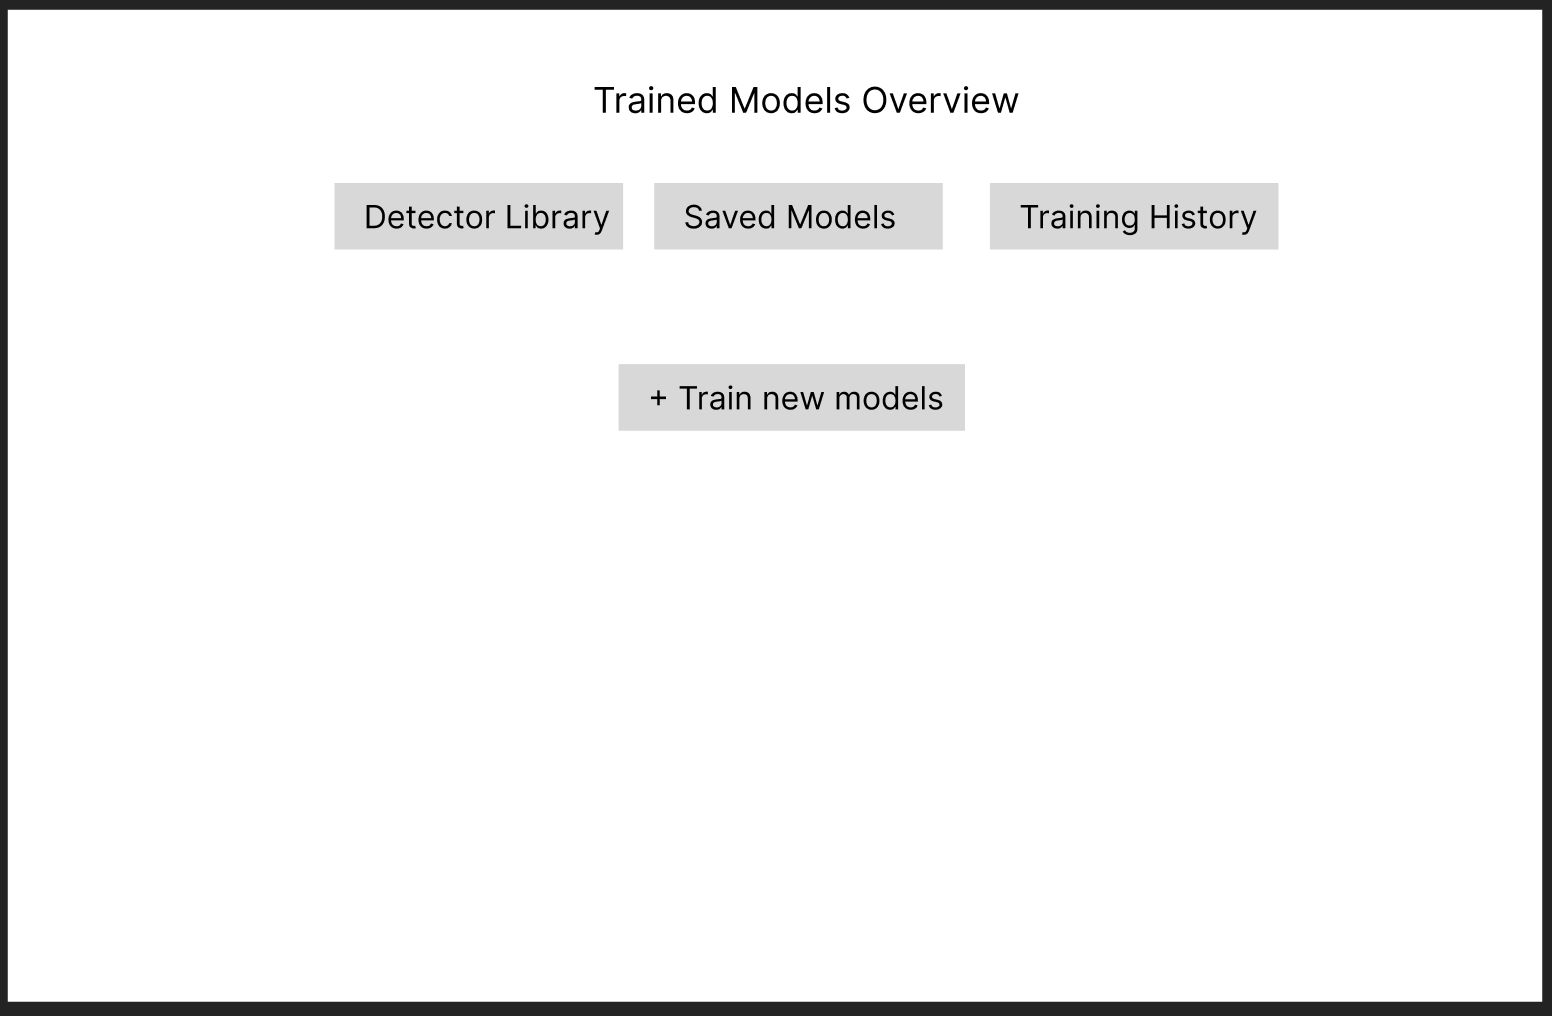
\includegraphics[width=1\linewidth]{figures/design/Training_and_importing/Screenshot 2026-09-24 at 01.17.15.png}
    \caption{Trained Models overview}
    \label{fig:trained_models_overview}
\end{figure}

\begin{figure}[H]
    \centering
    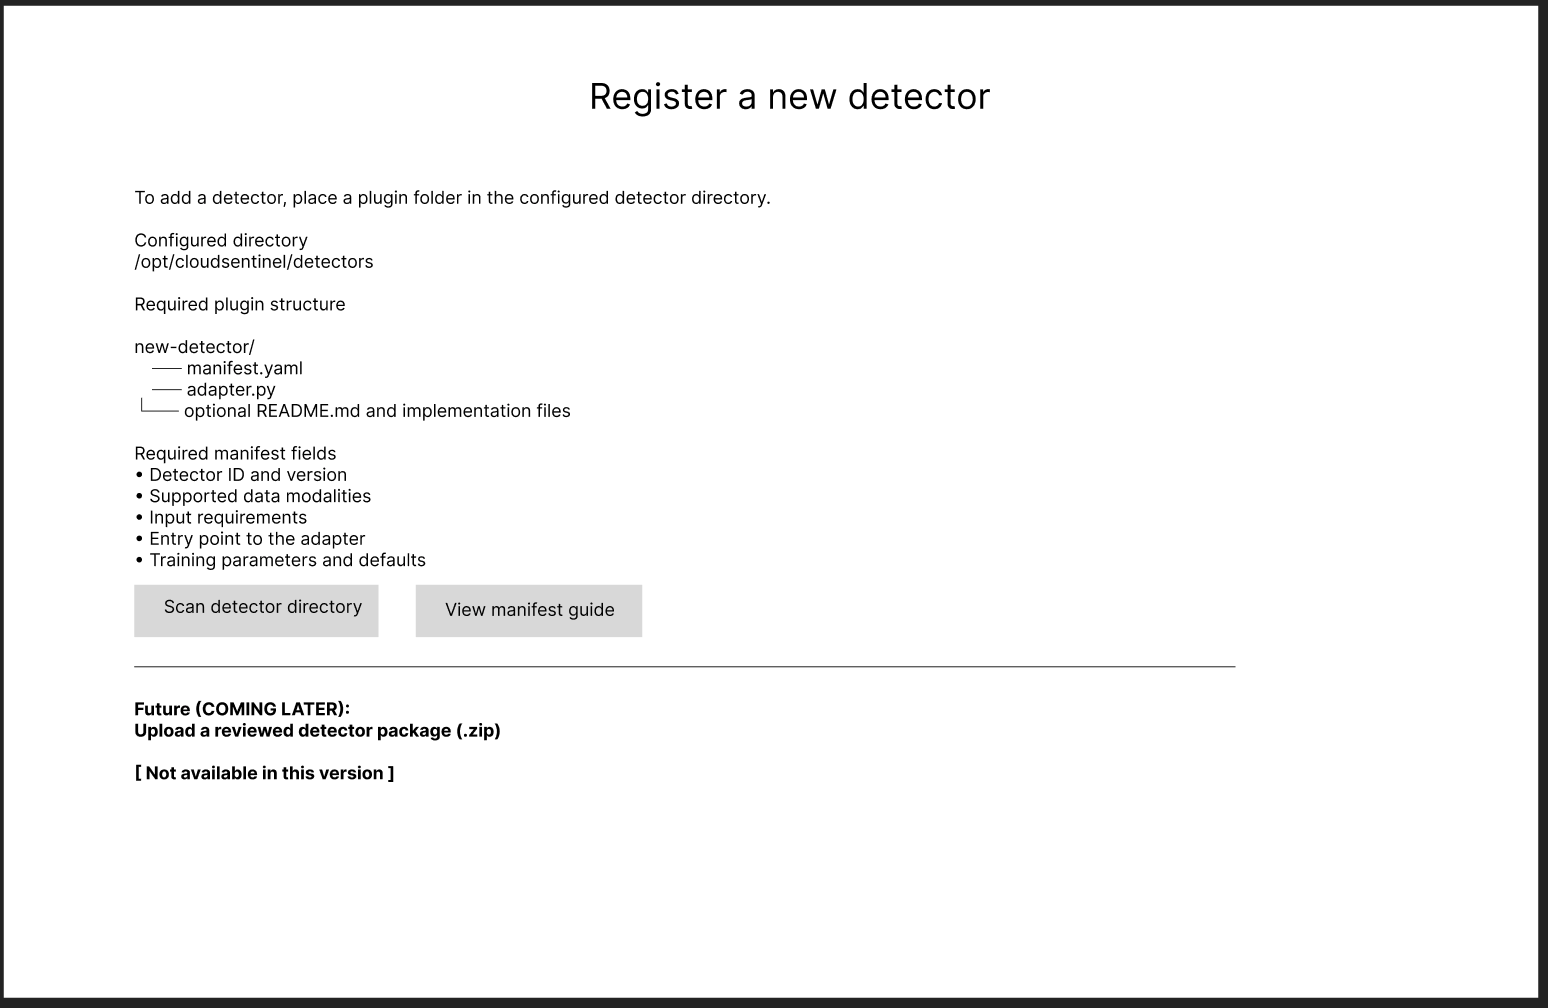
\includegraphics[width=1\linewidth]{figures/design/Training_and_importing/Screenshot 2026-09-24 at 01.17.23.png}
    \caption{Register a new detector}
    \label{fig:register_detector_model}
\end{figure}

\begin{figure}[H]
    \centering
    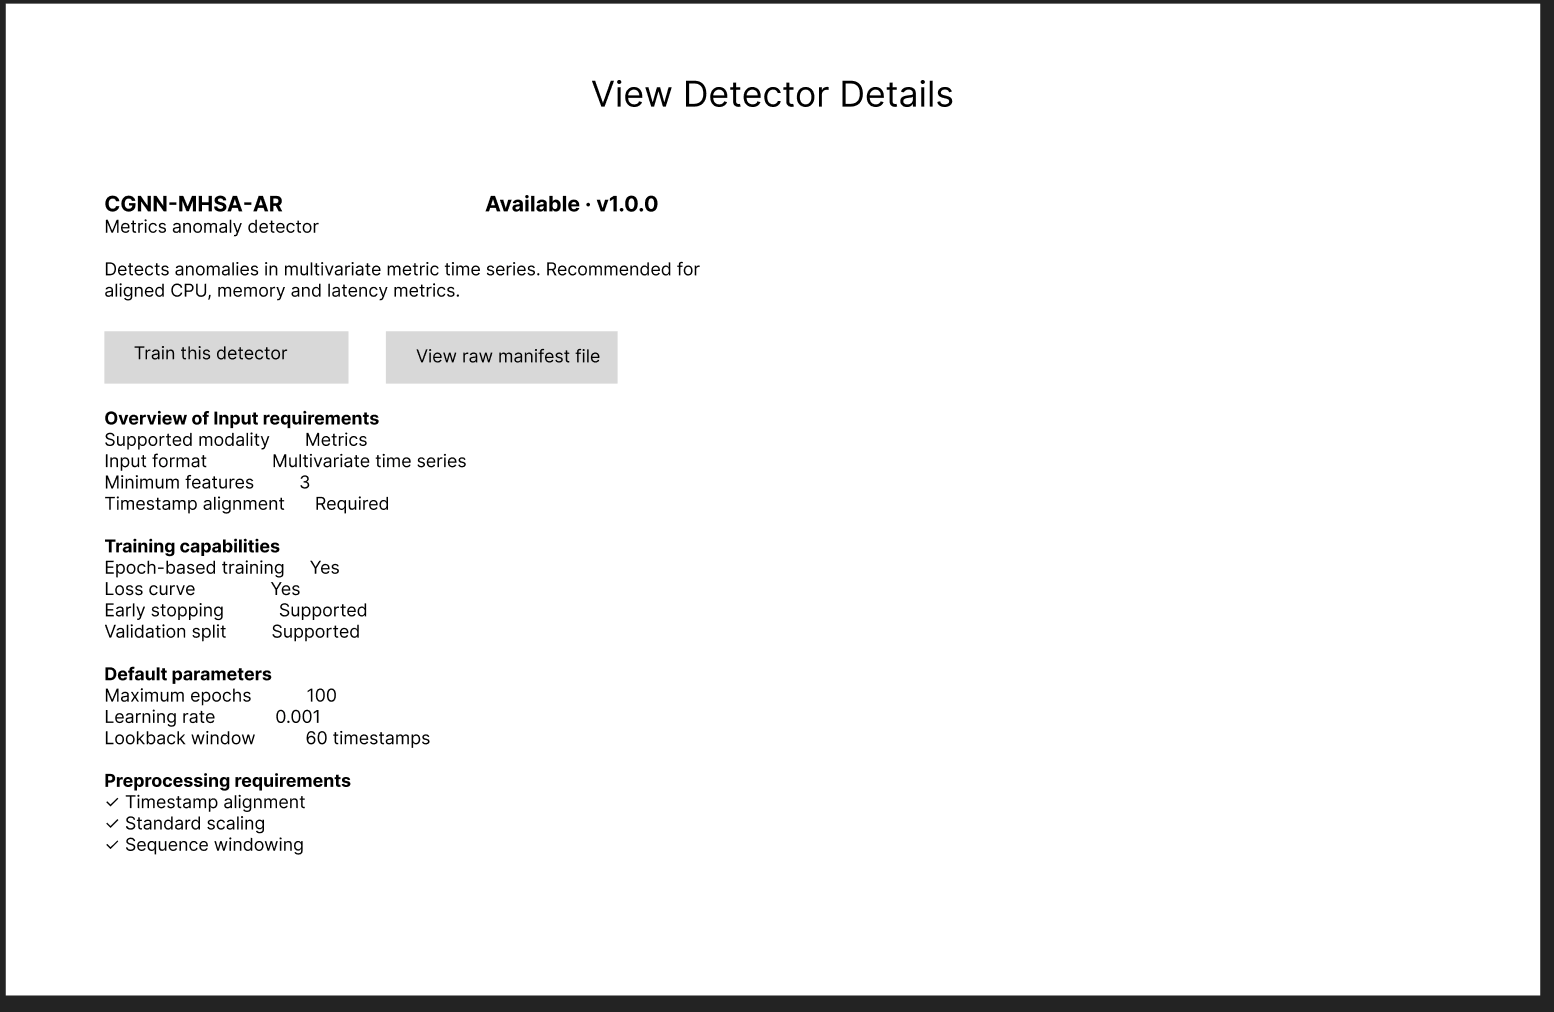
\includegraphics[width=1\linewidth]{figures/design/Training_and_importing/Screenshot 2026-09-24 at 01.17.34.png}
    \caption{View Detector Details}
    \label{fig:view_detector_details}
\end{figure}

\begin{figure}[H]
    \centering
    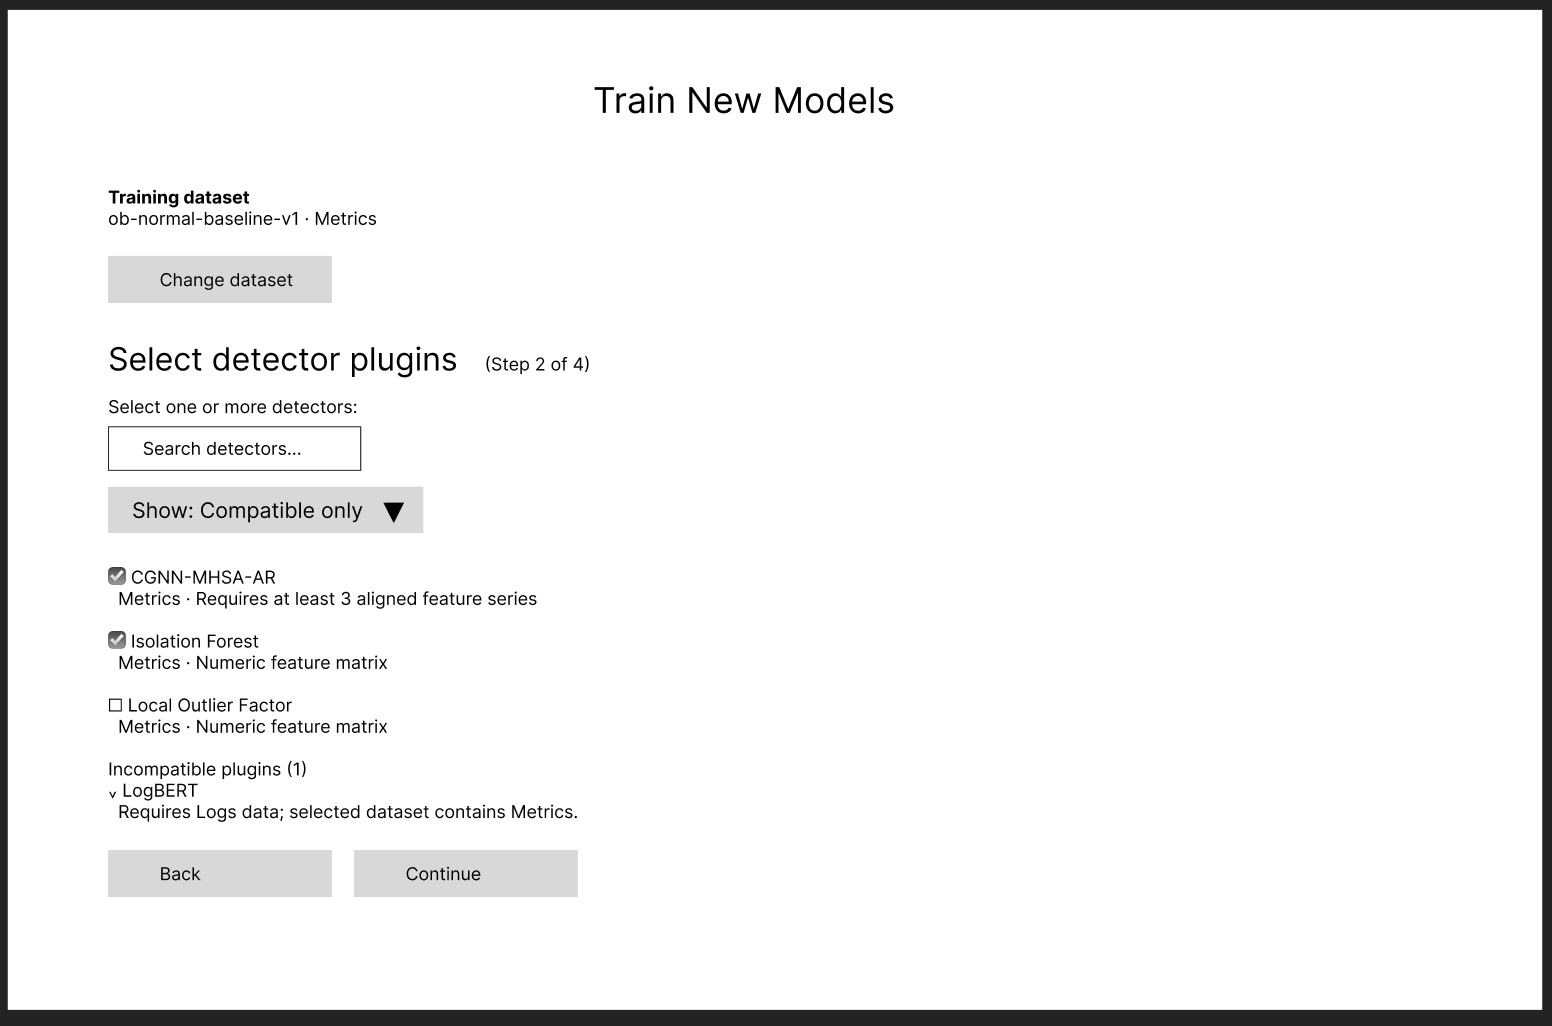
\includegraphics[width=1\linewidth]{figures/design/Training_and_importing/Screenshot 2026-09-24 at 01.17.53.png}
    \caption{Train New Models}
    \label{fig:train_new_models}
\end{figure}

% TRAINING MODELS USING THE DETECTORS
\begin{figure}[H]
    \centering
    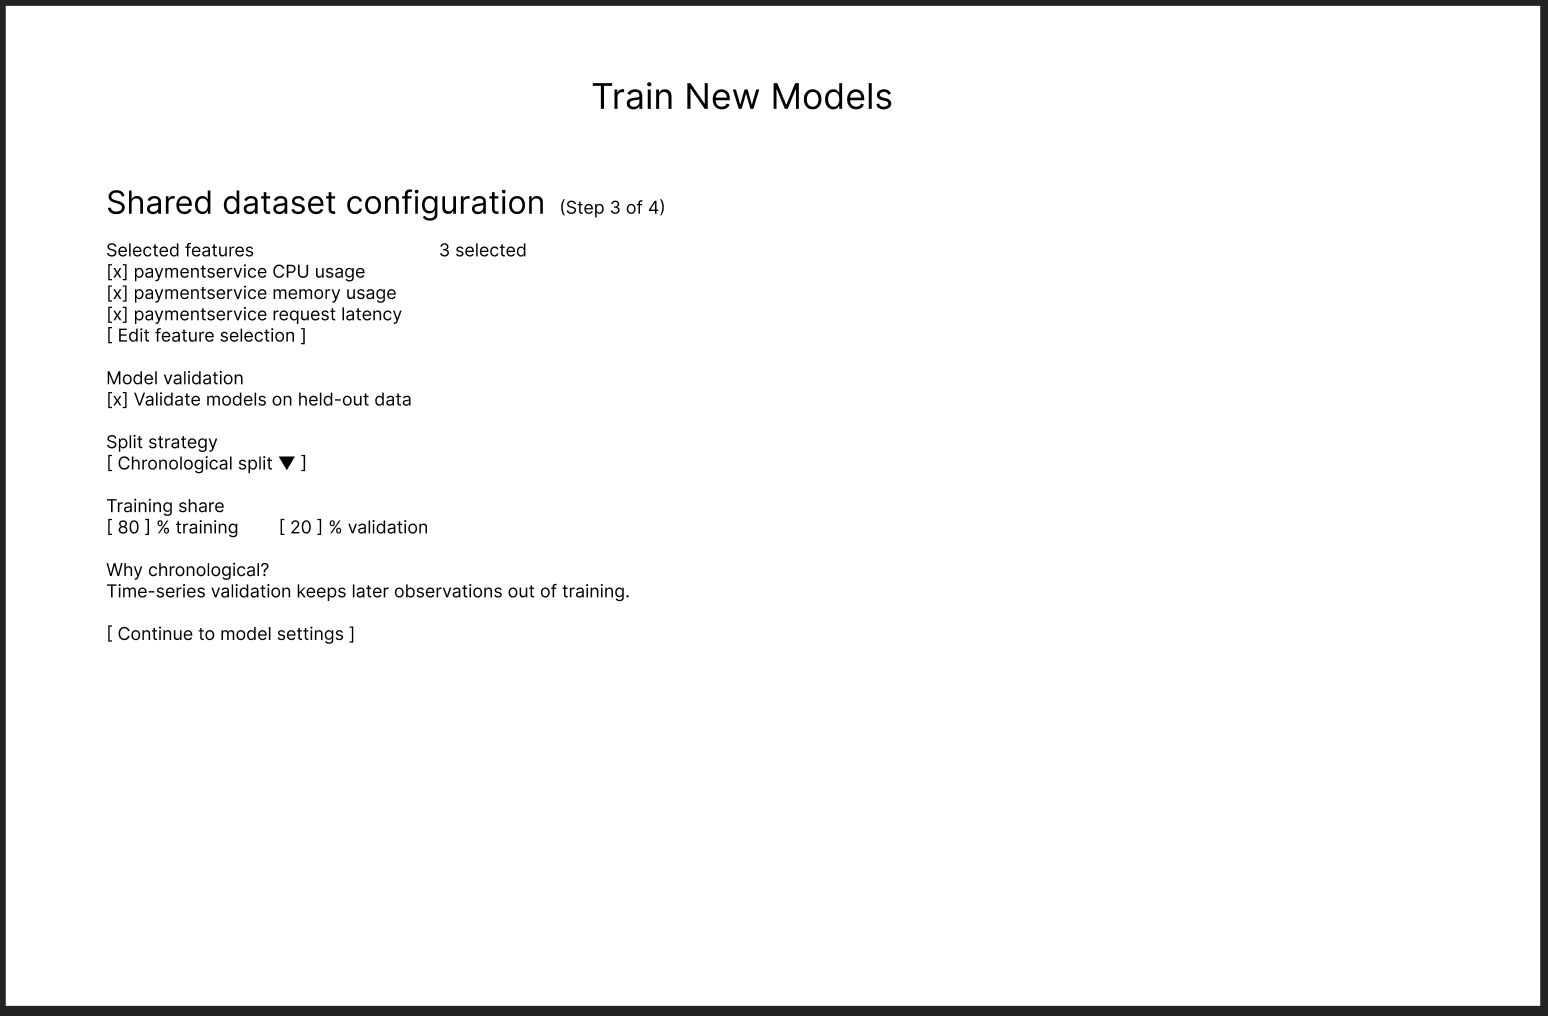
\includegraphics[width=1\linewidth]{figures/design/Training_and_importing/Screenshot 2026-09-24 at 01.18.01.png}
    \caption{Train New Models: Review Screen}
    \label{fig:train_review_screen}
\end{figure}

\subsection{Model Comparisons}
In order to make an assessment of what model to use, as well as being able to compare detector algorithms with each other, we introduce a Model Comparison component, which allows users to select a dataset with a given workload context (e.g. CPU usage spike anomaly), and run each model against the dataset, producing insightful evaluation metrics in the process that let operators compare their trained models. In order for the operator to be able to make an insightful assessment, three criteria points are applied. The first criterion is \textit{accuracy}, which is expressed as F1, precision and recall. The second criterion is \textit{lead time}, which is the time by which a model is able to predict an anomaly from occurring beforehand. The third criterion is \textit{robustness}, which we define as the degree to which a model is able to deliver consistent anomaly detection results across different workload contexts (for instance: low vs high activity datasets).\\

Figure \ref{fig:comparison_overview_screen} displays the comparison overview screen, which provides operators with a central location for managing previously executed anomaly-detection model comparisons. Rather than evaluating models in isolation, the design treats each comparison as a persistent evaluation artefact that records the evaluated models, the dataset used, and the resulting performance measures. This allows operators to revisit earlier evaluations, inspect their outcomes, and distinguish completed comparisons from those that still require execution or review.

Figure \ref{fig:comparison_new_comparison_screen} displays the 'new comparison' screen, which is essentially a guided workflow for the user for creating a new anomaly-detection comparison. The operator first selects a saved evaluation dataset and then chooses one or more trained model artefacts to evaluate on that same data. Requiring a shared evaluation dataset is important because it ensures that differences in the results can be attributed to the models and their configurations rather than to differences in input data. The review step makes the selected dataset, models, incident context, and intended evaluation measures visible before execution. This helps prevent accidental comparisons of incompatible artefacts and supports a more reproducible evaluation workflow.

Finally, figure \ref{fig:comparison_results_screen} displays the comparison results screen. This view brings together the information required to interpret model behaviour in one place. It presents a summary of the compared models and their evaluation measures, including precision, recall, F1-score, and lead time, while also retaining the associated training dataset and detection threshold for each model. The timeline view links model scores and thresholds to the known anomaly interval, enabling operators to inspect not only aggregate performance but also when each model identified anomalous behaviour. In addition, the detailed model view and provenance links allow the user to trace an observed result back to the model and training data that produced it. The design therefore supports a more informed model-selection process than relying on a single score or an untraceable trained artefact.

\begin{figure}[H]
    \centering
    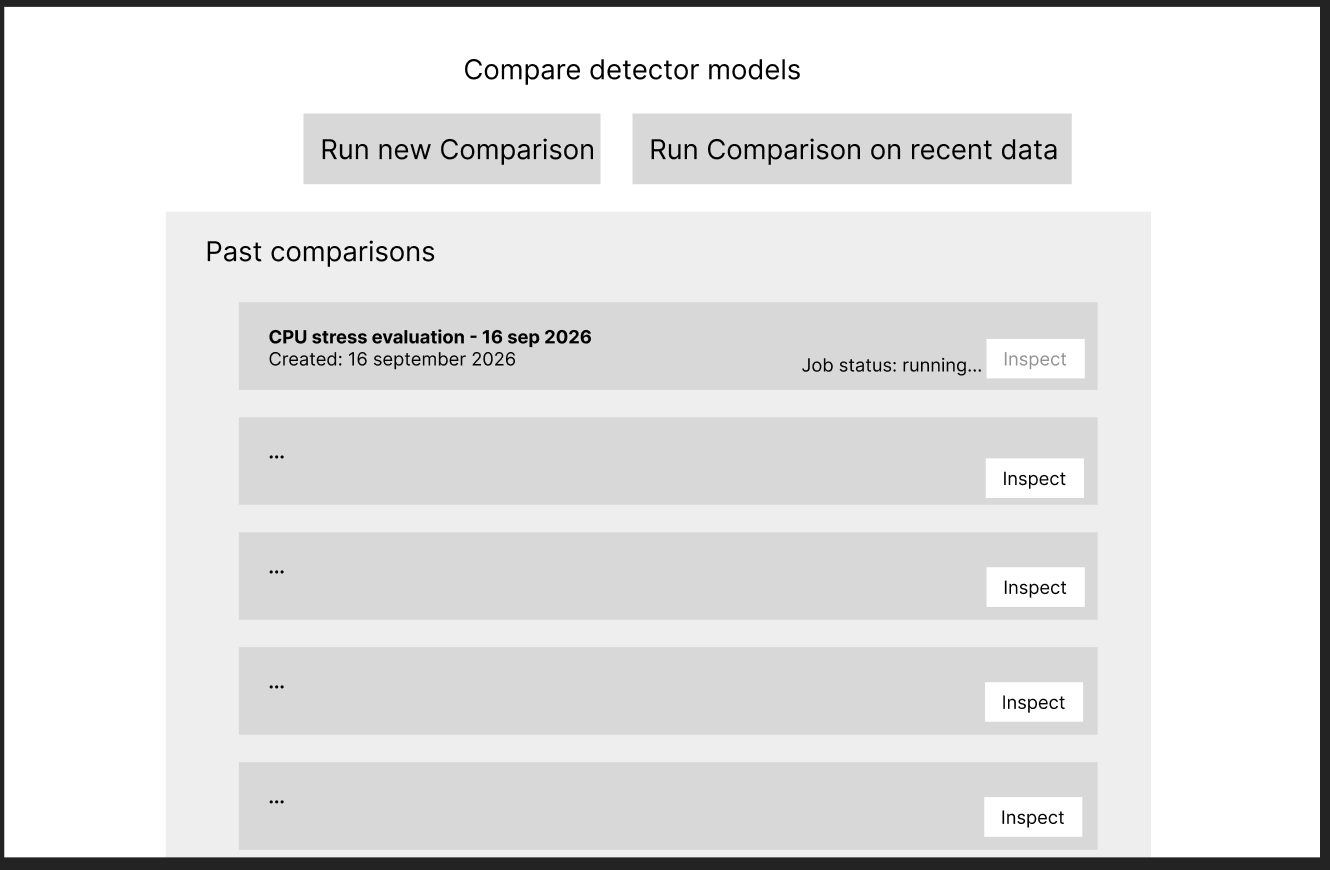
\includegraphics[width=1\linewidth]{figures/design/model_comparisons/Screenshot 2026-09-24 at 00.41.24.png}
    \caption{Compare Detector Models: Overview screen}
    \label{fig:comparison_overview_screen}
\end{figure}

\begin{figure}[H]
    \centering
    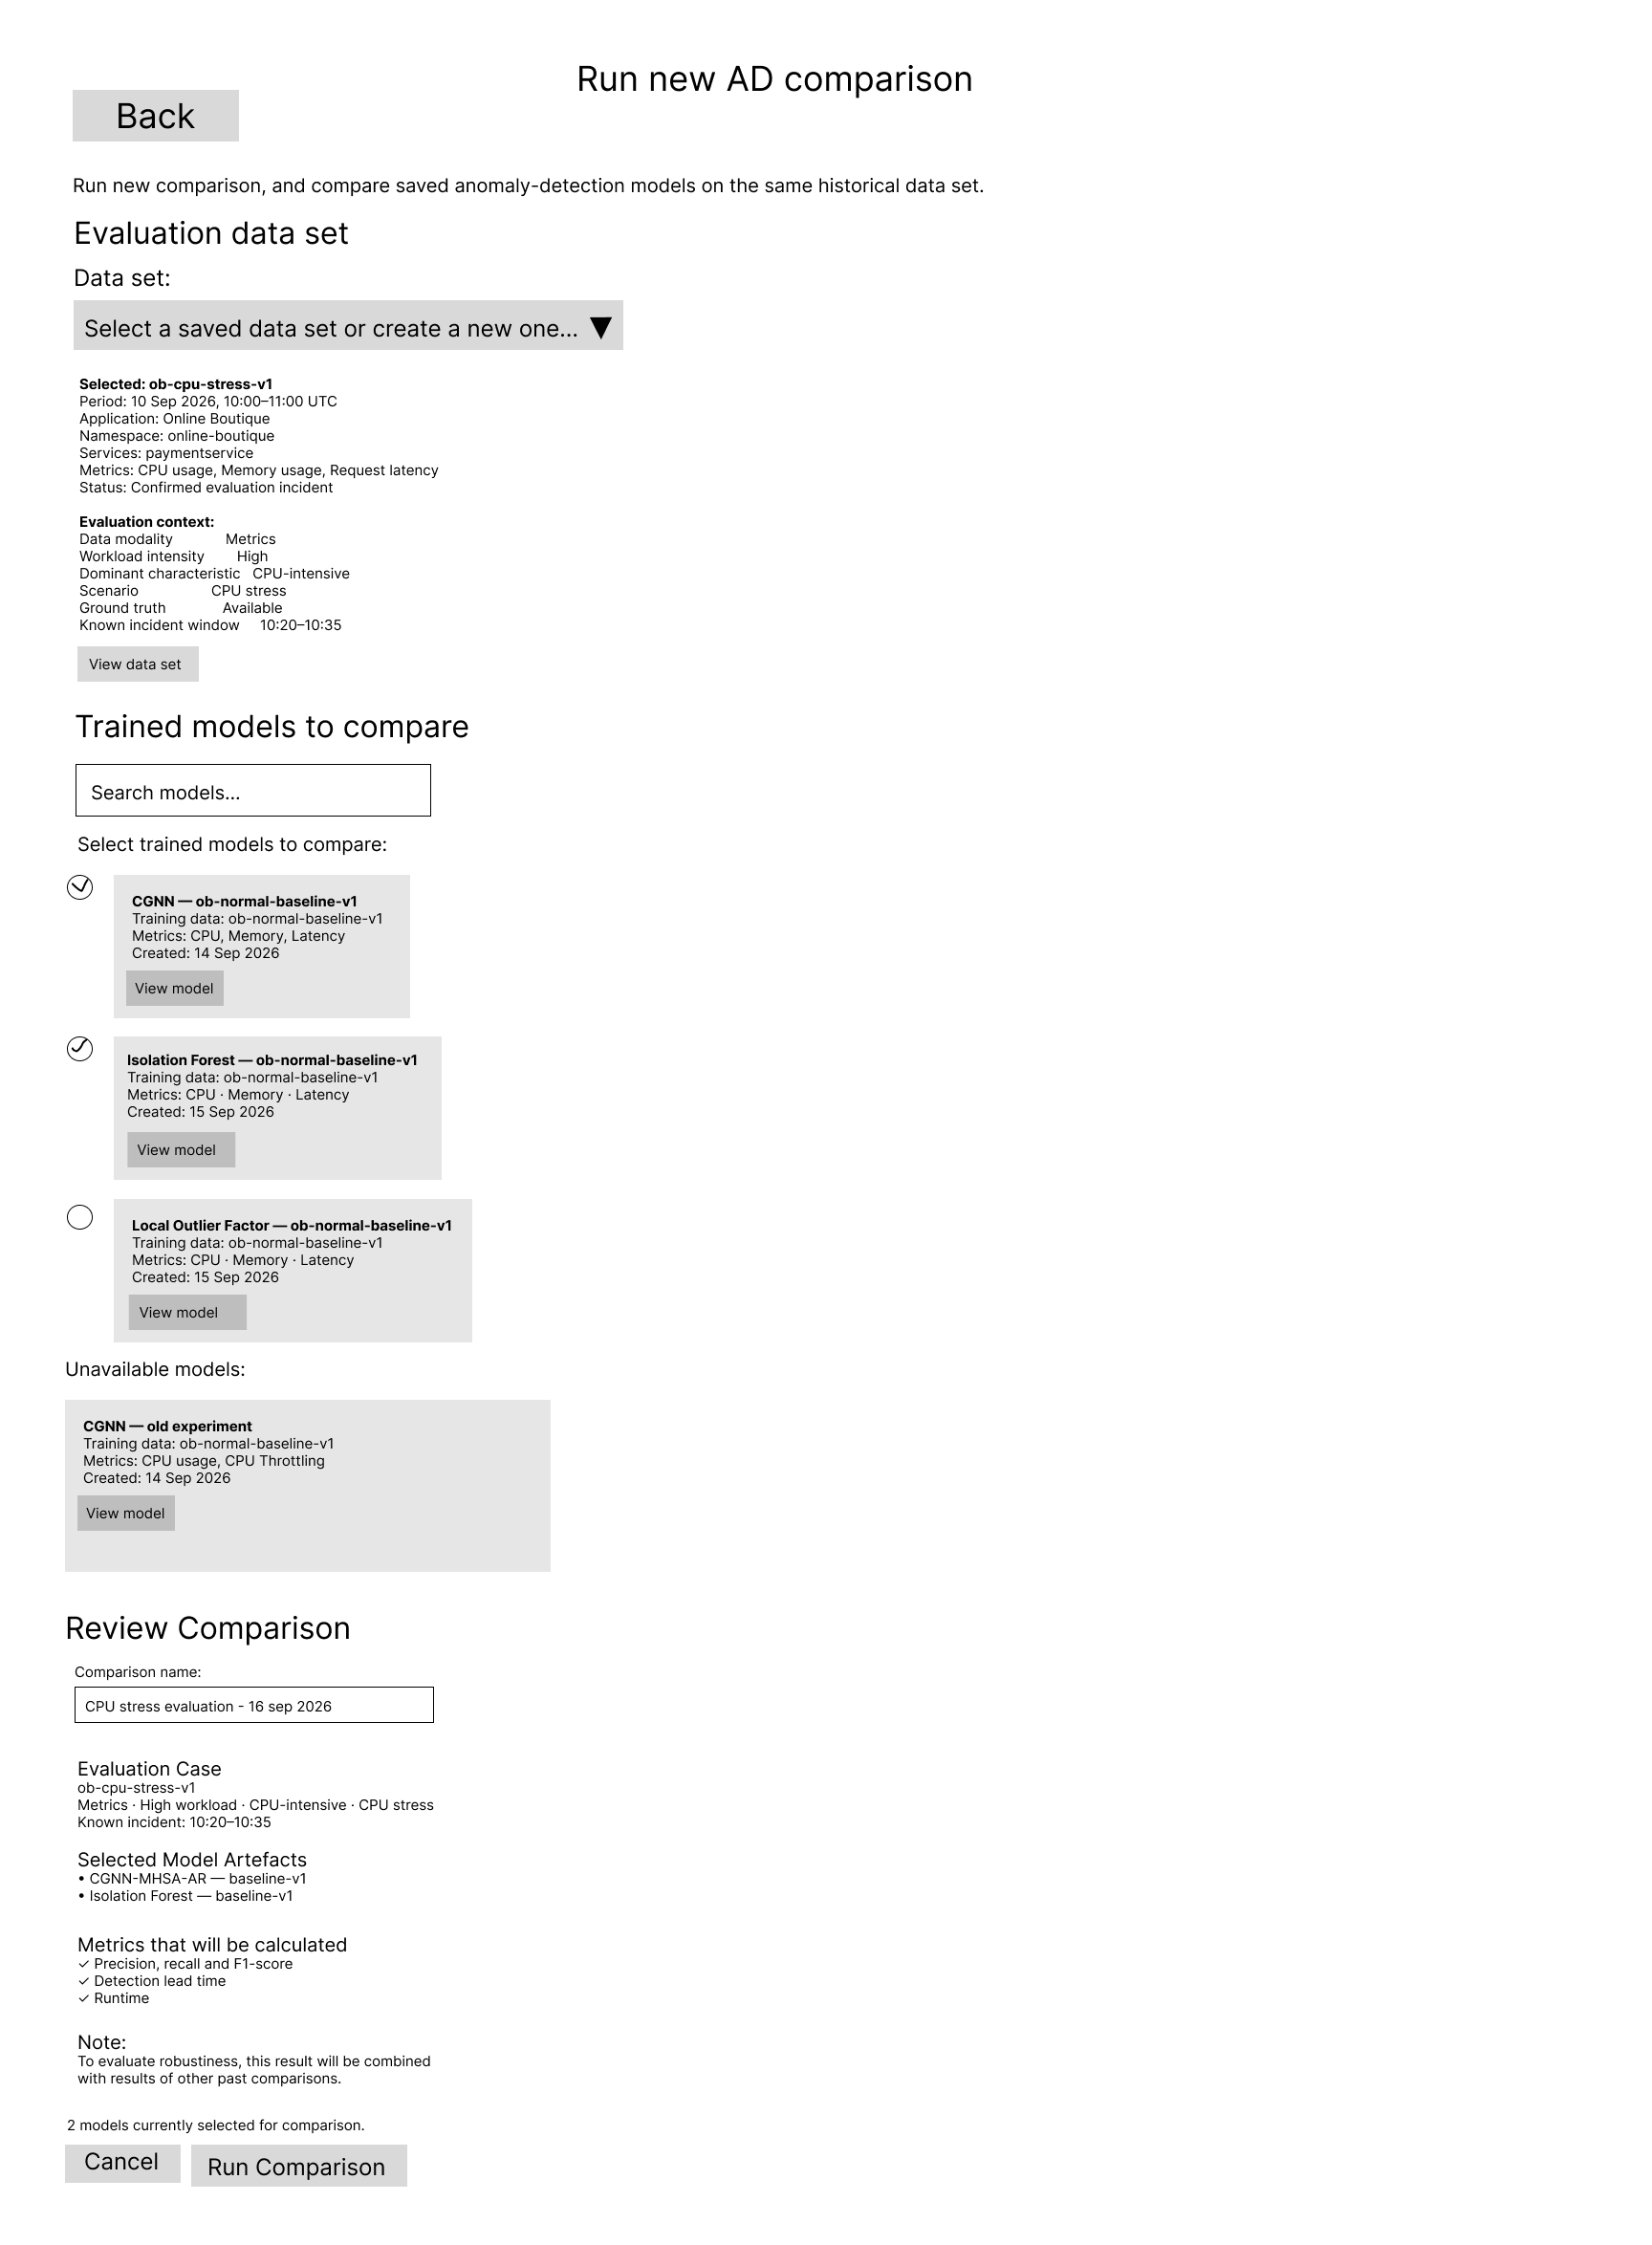
\includegraphics[width=1\linewidth]{figures/design/model_comparisons/Compare AD models - run new comparison.png}
    \caption{'Run new comparison' screen}
    \label{fig:comparison_new_comparison_screen}
\end{figure}

\begin{figure}[H]
    \centering
    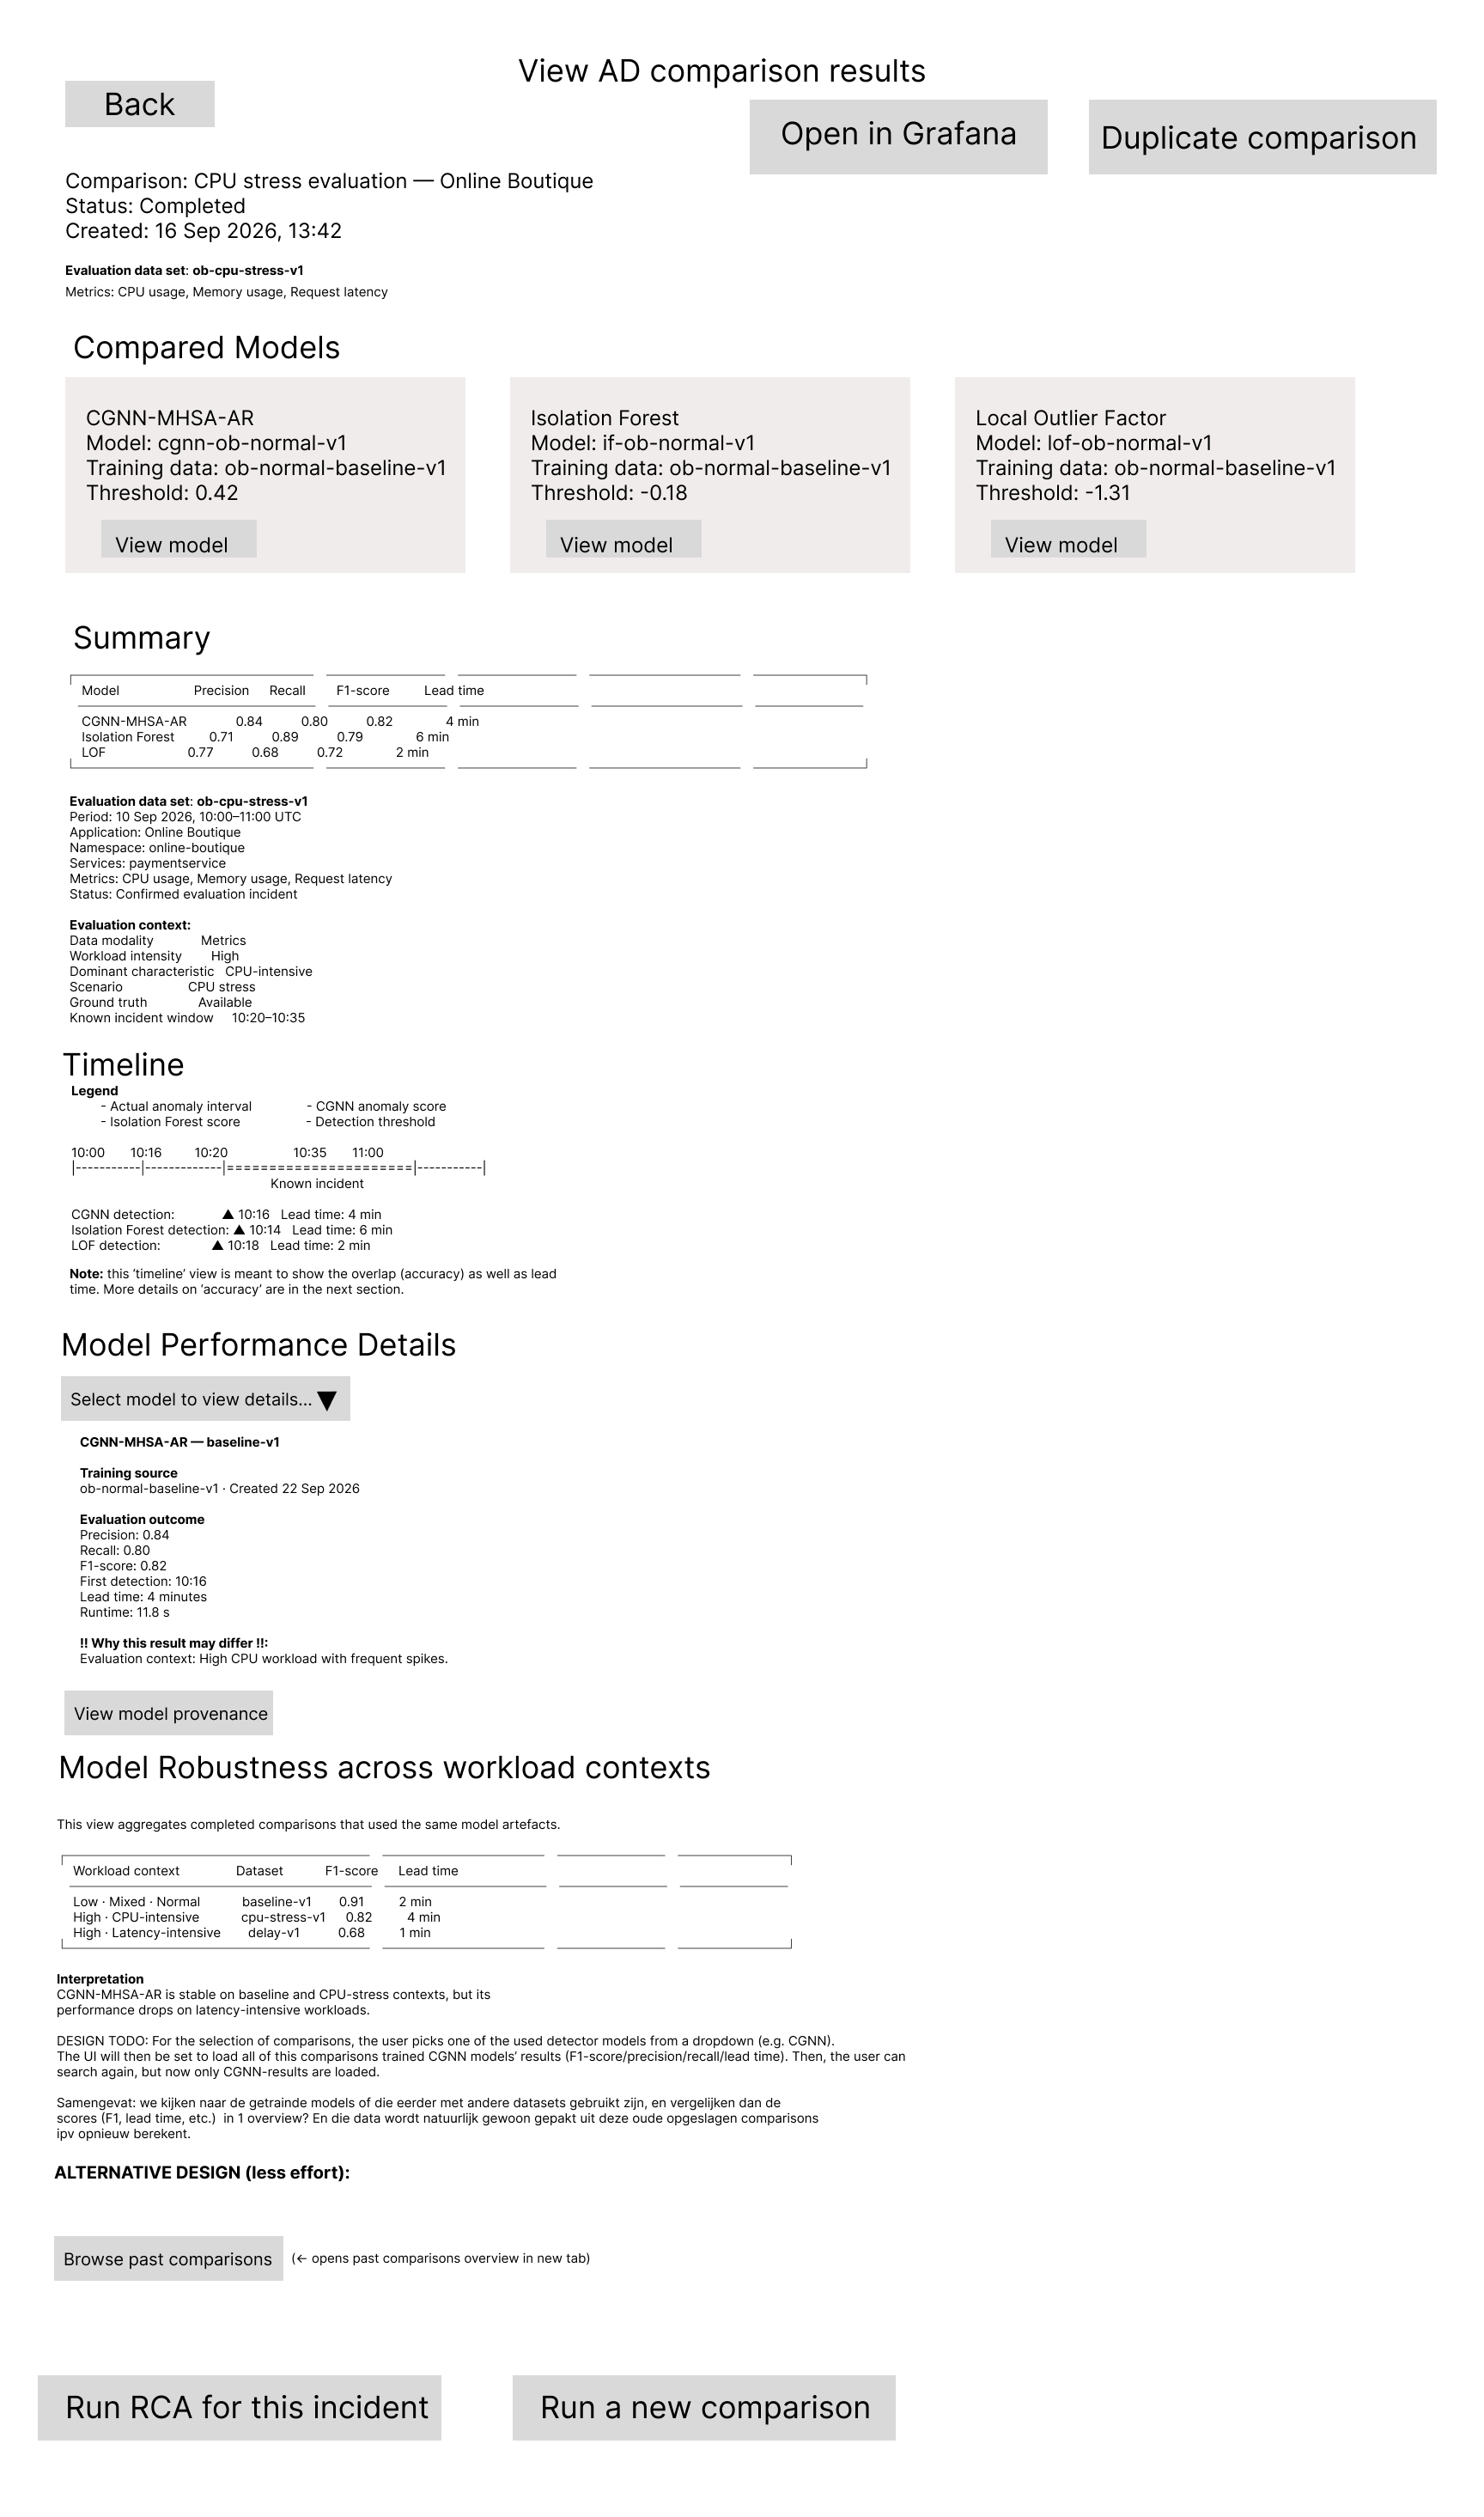
\includegraphics[width=1\linewidth]{figures/design/model_comparisons/comparison results.png}
    \caption{Comparison Results}
    \label{fig:comparison_results_screen}
\end{figure}

\subsection{Revised Live Monitoring}

The existing live-monitoring workflow also needs to be revised so that it continues to work with the other proposed changes. In the baseline framework, live monitoring is closely connected to the CGNN implementation and its own data-preparation and detection routes. This no longer fits a framework in which several detector plugins can produce Saved Models with different preprocessing and artefact formats.

The revised design therefore starts monitoring from one explicit Saved Model rather than from a general detector type. The monitoring pipeline should collect live Prometheus observations in the same feature order and with the same source configuration as the data used to prepare that model. It should then send these observations to the generic inference interface provided by the model's detector adapter. In this way, live monitoring can use CGNN, Isolation Forest, Local Outlier Factor, or a later compatible detector without adding a separate monitoring route for each one.

The monitoring interface should also retain the identity of the selected model and present the resulting anomaly information as a named session. Where the selected input and available monitoring evidence are suitable, an operator should be able to enable root-cause analysis for that session. The detailed monitoring-history and selectable RCA functions described later were not fully specified in the initial design. They were added during implementation after it became clear that short-lived task results were insufficient for revisiting and explaining live detections.

\section{Implementation}
The implementation connects the previously separate parts of CloudSentinel into one experimental workflow. A researcher can start with live Prometheus data or an imported CSV file, prepare a dataset, train compatible detectors, compare the resulting model artefacts, and continue with live monitoring and RCA. The interface carries the selected dataset, run, comparison, and model forward where possible. This does not remove every configuration decision, but it makes the relationship between the steps visible and keeps their evidence connected.

\begin{figure}[H]
    \centering
    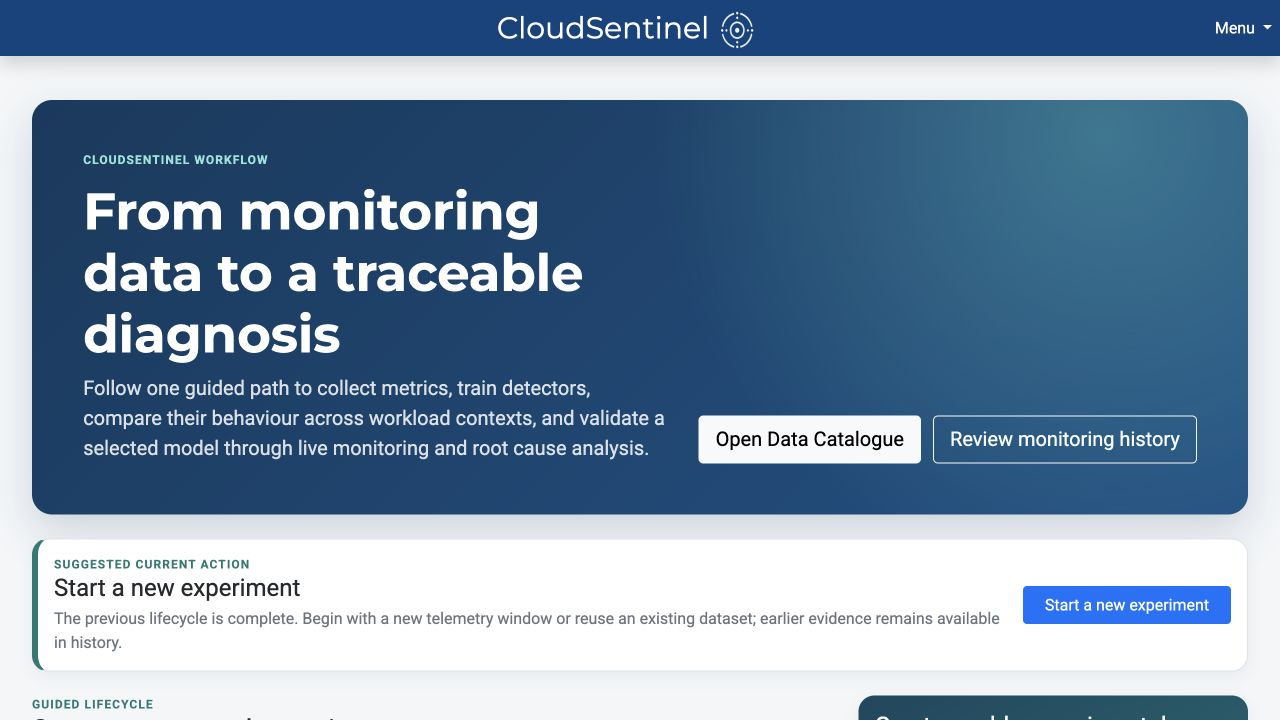
\includegraphics[width=1\linewidth]{figures/implementation/current/workflow_overview.jpg}
    \caption{Workflow overview showing the connected route from monitoring data to stored detection and diagnosis evidence.}
    \label{fig:overview}
\end{figure}

The workflow overview in Figure~\ref{fig:overview} gives one recommended next action based on the artefacts that already exist. After a completed experiment, it offers a new start instead of leaving the homepage permanently at the final monitoring step. A small guide remains visible on the detailed pages and provides direct continuation links, for example from a completed training run to a new comparison.

The monitored environment is configured centrally. An operator supplies the Prometheus address, Kubernetes namespace, and, when required, authentication and TLS settings. Secrets are stored on the server and are never repeated in dataset or model records. Grafana is optional. When it is configured, the Data Catalogue, telemetry explorer, workload page, and monitoring page provide direct links to Grafana and Prometheus. CloudSentinel also contains a small telemetry explorer for the common case in which a researcher first wants to inspect recent behaviour and then capture the corresponding time window as a dataset.

\subsection{Data Catalogue}
The Data Catalogue was implemented as an extension of CloudSentinel's existing data-ingestion and user-interface components. Its purpose is to turn a description of a Prometheus time window into a reusable dataset with a stable identity, recorded origin, and explicit training or evaluation partition. The implementation therefore covers more than a page that lists files. It includes dataset metadata, data collection, validation, versioning, ground-truth annotations, partitioning, and the controlled transfer of data to the model-training pipeline.

\subsubsection{Implementation overview}

Figure~\ref{fig:data_catalogue_implementation_architecture} shows the main components involved. The operator uses pages implemented in the existing Django user-interface service. These pages do not access Prometheus or catalogue files directly. Instead, a server-side catalogue client sends HTTP requests to a Flask blueprint in the data-ingestion service. This blueprint exposes the dataset operations and uses a file-backed repository for catalogue metadata and artefacts.

Fetching a dataset can take longer than a normal web request. It is therefore executed by a Celery worker rather than by the API process. The API validates the request, records a fetch attempt, and dispatches a task through Redis. The worker then queries the configured Prometheus instance and writes its results to the shared catalogue volume. The API and worker mount the same volume, which means that a dataset created through the interface remains available after a process or pod restart. The learning-adaptation service accesses catalogue data through an HTTP endpoint that produces a verified training bundle; it does not read the catalogue directory directly.

\begin{figure}[H]
    \centering
    \resizebox{0.98\linewidth}{!}{%
    \begin{tikzpicture}[
        font=\small,
        node distance=11mm and 10mm,
        component/.style={draw, rounded corners=2pt, align=center, minimum height=10mm, text width=27mm, fill=blue!7},
        external/.style={draw, rounded corners=2pt, align=center, minimum height=10mm, text width=25mm, fill=orange!12},
        storage/.style={draw, cylinder, shape border rotate=90, aspect=0.25, align=center, minimum height=13mm, text width=28mm, fill=green!10},
        flow/.style={-{Latex[length=2mm]}, thick},
        dataflow/.style={-{Latex[length=2mm]}, thick, dashed}
    ]
        \node[component] (ui) {Django user interface};
        \node[component, right=of ui] (api) {Data Catalogue API\\in data ingestion};
        \node[component, right=of api] (worker) {Celery data-ingestion worker};
        \node[external, right=of worker] (prometheus) {Prometheus\\\texttt{query\_range}};
        \node[component, below=17mm of ui] (learning) {Learning-adaptation service};
        \node[storage, below=17mm of api, xshift=20mm] (storage) {Catalogue persistent volume};

        \draw[flow] (ui) -- node[above, font=\scriptsize] {HTTP} (api);
        \draw[flow] (api) -- node[above, font=\scriptsize] {task via Redis} (worker);
        \draw[flow] (worker) -- node[above, font=\scriptsize] {PromQL} (prometheus);
        \draw[flow] (prometheus) to[bend left=18] node[below, font=\scriptsize] {time series} (worker);
        \draw[flow] (api) -- (storage);
        \draw[flow] (worker) -- (storage);
        \draw[dataflow] (learning) -- node[above, font=\scriptsize, align=center] {request exact\\training bundle} (api);
    \end{tikzpicture}%
    }
    \caption{Implemented Data Catalogue architecture. Dataset management is exposed by the data-ingestion API, while Prometheus collection is performed asynchronously by a worker.}
    \label{fig:data_catalogue_implementation_architecture}
\end{figure}

The catalogue was added to the data-ingestion service instead of being introduced as a separate microservice. This keeps the responsibility for collecting and storing input data in the component that already communicates with monitoring sources. Existing datasets from the earlier CloudSentinel directory structure are projected into the catalogue as read-only records. This compatibility layer allows the new training workflow to use older datasets without rewriting or moving their original CSV files.

\subsubsection{Dataset representation and versioning}

The implementation separates a logical dataset from a specific version of its data. A logical dataset has a generated identifier such as \texttt{ds\_<uuid>} and stores descriptive fields that may change over time: its display name, description, purpose, tags, and current workload context. Changes to these fields increase a metadata revision counter and are recorded in a small change history. The logical record also points to the latest version and contains summaries that are used by the overview page.

A dataset version stores the information required to reproduce one exact collection request. This includes the Prometheus source identifier, application and namespace, requested services or pods, start and end time, sampling interval, PromQL query templates, workload context, feature order, validation result, and references to the resulting artefacts. A newly created dataset starts at version~1 with status \texttt{draft}. A later version can copy an existing source configuration and then change its time window, queries, workload context, or partition. The previous version remains available.

The source configuration becomes frozen as soon as fetching starts. A user cannot silently change the query or time window of data that has already been collected. If a different collection is required, the system creates a new version. This distinction is important for provenance: a trained model can refer to a dataset identifier, version number, and partition identifier instead of only to a filename whose contents may later change.

Figure~\ref{fig:data_catalogue_storage_model} summarises the file-backed representation. The logical record and version documents are JSON files. Collected data and provenance are stored under the corresponding version number, while incidents, labels, and partition definitions are stored as overlays. An overlay adds interpretation to an available version but does not rewrite its original Prometheus request or canonical observations.

\begin{figure}[H]
    \centering
    \resizebox{0.98\linewidth}{!}{%
    \begin{tikzpicture}[
        font=\small,
        node distance=10mm and 11mm,
        box/.style={draw, rounded corners=2pt, align=left, minimum height=11mm, text width=38mm, fill=blue!6},
        child/.style={draw, rounded corners=2pt, align=left, minimum height=12mm, text width=39mm, fill=gray!10},
        overlay/.style={draw, rounded corners=2pt, align=left, minimum height=12mm, text width=39mm, fill=green!9},
        link/.style={-{Latex[length=2mm]}, thick}
    ]
        \node[box] (record) {\textbf{Logical dataset}\\\texttt{dataset.json}\\name, purpose, metadata history};
        \node[box, right=18mm of record] (version) {\textbf{Immutable version}\\\texttt{versions/000001.json}\\source request, schema, checksums};
        \node[child, below=of version, xshift=-26mm] (artifacts) {\textbf{Collected artefacts}\\raw responses, canonical CSV files, provenance and validation};
        \node[overlay, below=of version, xshift=26mm] (overlays) {\textbf{Version overlays}\\incident windows, row labels and partition definitions};

        \draw[link] (record) -- node[above, font=\scriptsize] {has versions} (version);
        \draw[link] (version) -- (artifacts);
        \draw[link] (version) -- (overlays);
    \end{tikzpicture}%
    }
    \caption{Separation between mutable descriptive metadata, immutable dataset versions, collected artefacts, and version-specific overlays.}
    \label{fig:data_catalogue_storage_model}
\end{figure}

\subsubsection{Collecting data from Prometheus}

When an operator saves a dataset, the API first validates the complete configuration. The dataset form does not accept a Prometheus URL or credentials. It submits a server-defined source identifier, which the data-ingestion service resolves against the central monitored-environment configuration. This keeps connection details and secrets outside dataset records and prevents a catalogue request from silently redirecting the worker to another endpoint.

Each configured query has a query identifier, display name, feature name, PromQL template, and a flag that states whether the query is required. Templates may use controlled placeholders for the namespace, pod, and service. Before dispatch, the API resolves the requested targets, expands the templates, and estimates the maximum number of samples. Configurable limits restrict the query count and length, time-window size, minimum sampling interval, number of series, response size, retry count, and request timeouts. In the current default configuration, a request may contain at most 25 queries, span at most 31 days, use an interval of at least five seconds, and produce at most two million theoretical samples. These bounds prevent a single interface request from starting an unbounded Prometheus query.

The fetch lifecycle is shown in Figure~\ref{fig:data_catalogue_fetch_lifecycle}. A draft enters the \texttt{fetching} state after the API has created an attempt record and successfully dispatched the worker task. The worker uses Prometheus' range-query endpoint for every resolved query and stores the unmodified JSON response in a staging directory. Progress can be requested through the API and is shown in the interface without keeping the original HTTP request open.

After all queries have completed, the worker constructs one canonical UTC time grid from the requested start time, end time, and sampling interval. Returned series are sorted and assigned stable feature names. Their samples are placed on this grid to produce \texttt{observations.csv}, \texttt{feature\_matrix.csv}, and \texttt{timestamps.csv}. A missing Prometheus sample remains empty. The catalogue deliberately performs no interpolation, imputation, scaling, windowing, or detector-specific preprocessing. Consequently, the stored dataset describes the collected observations rather than the assumptions of one particular detector.

\begin{figure}[H]
    \centering
    \resizebox{0.98\linewidth}{!}{%
    \begin{tikzpicture}[
        font=\small,
        node distance=9mm,
        state/.style={draw, rounded corners=2pt, align=center, minimum height=10mm, text width=25mm, fill=blue!7},
        success/.style={draw, rounded corners=2pt, align=center, minimum height=10mm, text width=25mm, fill=green!12},
        failure/.style={draw, rounded corners=2pt, align=center, minimum height=10mm, text width=25mm, fill=red!8},
        flow/.style={-{Latex[length=2mm]}, thick}
    ]
        \node[state] (draft) {\texttt{draft}\\configuration saved};
        \node[state, right=of draft] (fetching) {\texttt{fetching}\\queries executed};
        \node[state, right=of fetching] (validating) {\texttt{validating}\\matrix assembled};
        \node[success, right=of validating] (available) {\texttt{available}\\artefacts promoted};
        \node[failure, below=12mm of validating] (failed) {\texttt{failed}\\safe error recorded};

        \draw[flow] (draft) -- (fetching);
        \draw[flow] (fetching) -- (validating);
        \draw[flow] (validating) -- (available);
        \draw[flow] (fetching) -- (failed);
        \draw[flow] (validating) -- (failed);
        \draw[flow] (failed.west) to[bend right=28] node[below, font=\scriptsize] {retry} (fetching.south);
    \end{tikzpicture}%
    }
    \caption{State transitions of one dataset version during Prometheus collection. Failed attempts can be retried, while an available version is not overwritten.}
    \label{fig:data_catalogue_fetch_lifecycle}
\end{figure}

\subsubsection{Storage, validation and integrity}

The worker does not write directly to the active artefact directory. It first writes the request, raw responses, canonical files, schema, provenance, and validation result to a version- and attempt-specific staging directory. Only after all steps succeed is that directory renamed to the active artefact location. Renaming on the same volume is atomic, so API readers cannot observe a half-written dataset. When collection fails, the version receives status \texttt{failed}, a compact error is recorded, and incomplete staging data are not exposed as an available dataset.

Every promoted file receives a SHA-256 checksum. The version document records these checksums together with relative file paths and file sizes. Repository operations validate identifiers and resolve paths before reading or writing, preventing a crafted dataset identifier from escaping the configured storage root. JSON metadata updates are also written to a temporary file, flushed, and atomically replaced. These measures do not make the local repository a distributed database, but they do protect the single-node implementation against several common partial-write and path-handling errors.

The final schema records the number of observations and features, the exact feature order, missing-value counts, timestamp timezone, and the fact that no normalization or imputation was applied. Provenance records retain both the query templates and the resolved queries, their target, execution window, returned series and sample counts, response size, and warnings. This is the information needed to explain where a catalogue matrix came from and to detect if a later consumer receives different content.

\subsubsection{Ground truth and dataset partitions}

Incident information and labels are handled separately from the collected measurements. An incident window can be added only to an available version and must fall inside its source time window. It records a start and end time, scenario, affected services and metrics, and an optional annotation. Overlapping incident windows are rejected by default. This makes it possible to retain the operational context of a fault without claiming that the raw Prometheus data already contained row-level labels.

Labels can either be submitted explicitly or derived from the stored incident windows. In the latter case, each timestamp inside an incident interval, including its boundaries, receives label~1; all other timestamps receive label~0. The catalogue uses the fixed meaning \texttt{0 = normal} and \texttt{1 = anomaly}, and requires one label for every observation. An existing label artefact cannot be overwritten. A correction must therefore be represented by a new version instead of silently changing the evaluation ground truth.

The implementation supports three partition modes: none, predefined, and time range. The first leaves the version unpartitioned. A predefined partition represents the train and test files of a projected legacy dataset. A time-range partition selects explicit train and test intervals from canonical observations. These ranges must be inside the dataset window, may not overlap, and must each contain at least two observations. Each stored partition refers to the source version and feature order and receives both a unique partition identifier and a deterministic checksum. The identifier distinguishes stored definitions, while the checksum allows two otherwise identical definitions to be recognised as equivalent.

\subsubsection{Training readiness and materialisation}

Readiness is calculated rather than stored as a user-selected claim. A version supports unsupervised training when it is available and contains at least two observations and one feature. Labelled evaluation additionally requires row-level labels, an explicit train/test partition, and complete label coverage. The API returns both the Boolean result and the reasons why a dataset is not ready. The overview can therefore show readiness without hiding missing requirements from the operator. The unsupervised flag describes whether the matrix itself is suitable; the current version of the shared training bundle still requires labels because the existing CGNN and Isolation Forest training paths expect a labelled test set.

When training is started, the learning-adaptation service requests one exact dataset version and partition. The catalogue materialises these into a ZIP archive containing \texttt{manifest.json}, \texttt{train.csv}, \texttt{test.csv}, and \texttt{labels.csv}. The manifest pins the dataset version, partition identifier and checksum, feature order and its hash, label source, row counts, source-artefact checksums, and the checksum and byte size of every emitted CSV file. Materialisation again performs no scaling, imputation, or detector-specific transformation.

The learning-adaptation service streams the archive with a configured size limit and verifies its structure before accepting it. It rejects unexpected filenames or paths, symbolic links, identity mismatches, incorrect hashes, inconsistent feature counts, and incomplete labels. The verified files are then copied into an immutable training snapshot. The resulting training run retains the catalogue identifiers and hashes as provenance. This makes the relation from a trained model back to its precise input data explicit, even if the user later creates a newer version of the same logical dataset.

\subsubsection{User interface}

The Django interface exposes the backend operations as an operator workflow. Figure~\ref{fig:data_catalogue_ui_overview} shows the implemented overview. It combines free-text search with filters for lifecycle status, purpose, label availability, workload intensity, dominant workload characteristic, and anomaly scenario. Each result displays its version, matrix shape, label and partition state, time range, and calculated readiness. The overview therefore communicates whether a dataset merely exists or can already be used in training and evaluation.

\begin{figure}[H]
    \centering
    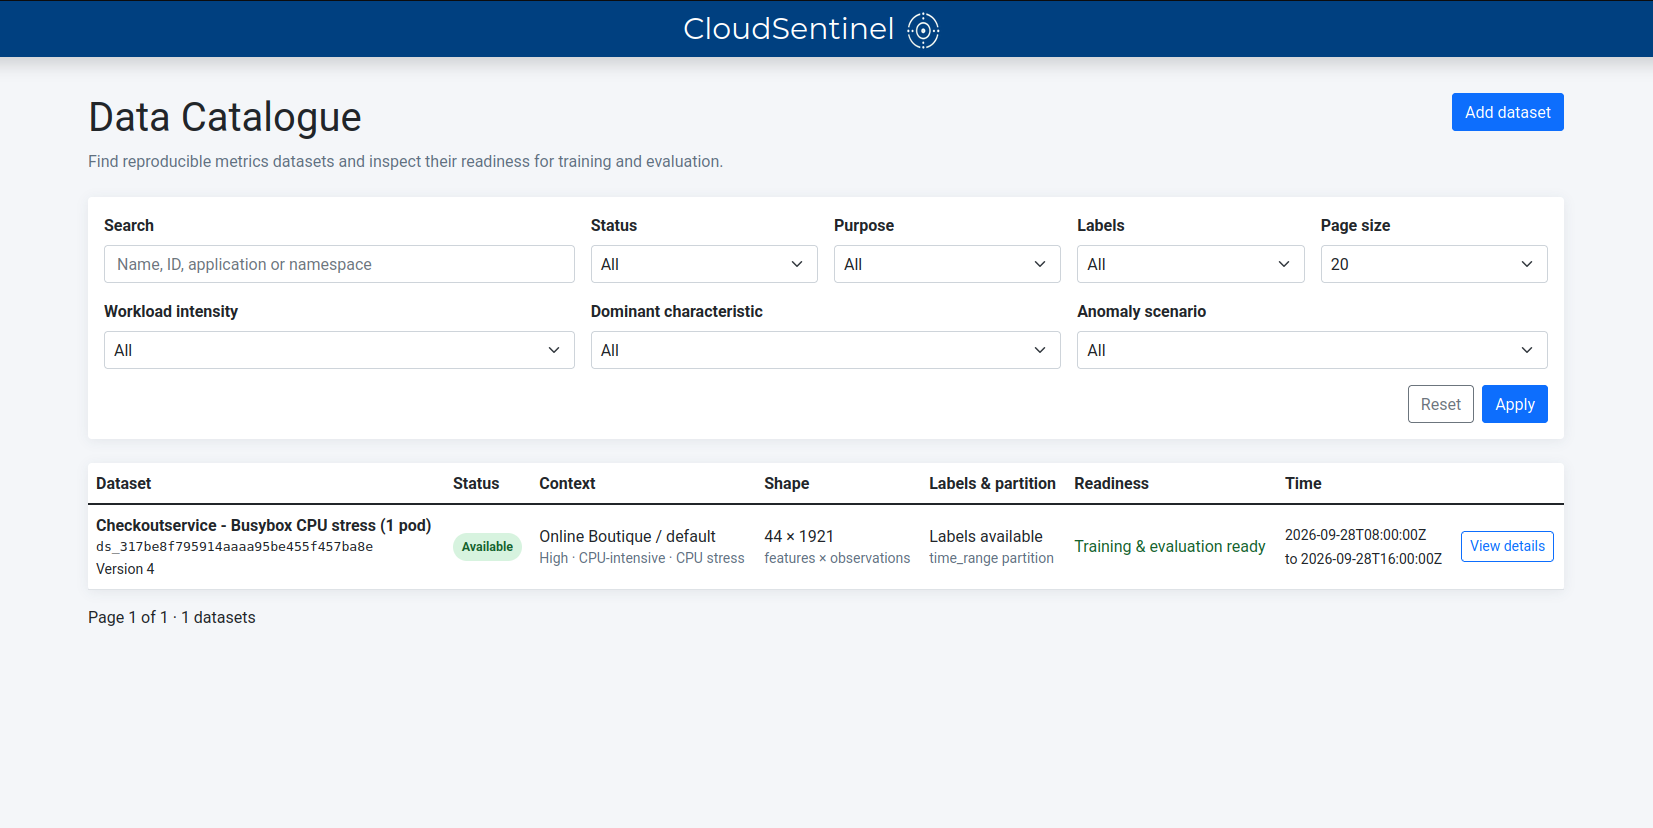
\includegraphics[width=1\linewidth]{figures/implementation/data_catalogue/Screenshot from 2026-10-06 17-18-47.png}
    \caption{Implemented Data Catalogue overview with search, context filters, dataset shape, label state, and calculated readiness.}
    \label{fig:data_catalogue_ui_overview}
\end{figure}

Figures~\ref{fig:data_catalogue_ui_add_source} and~\ref{fig:data_catalogue_ui_add_context} show the first parts of the dataset form. The operator enters descriptive metadata and a Prometheus time window, then defines one or more PromQL templates. Workload context is recorded through controlled fields rather than free text, which enables the filters on the overview and the later comparison of detector behaviour under different circumstances. Ground truth is optional: a dataset can first be collected for unsupervised training and annotated later.

\begin{figure}[H]
    \centering
    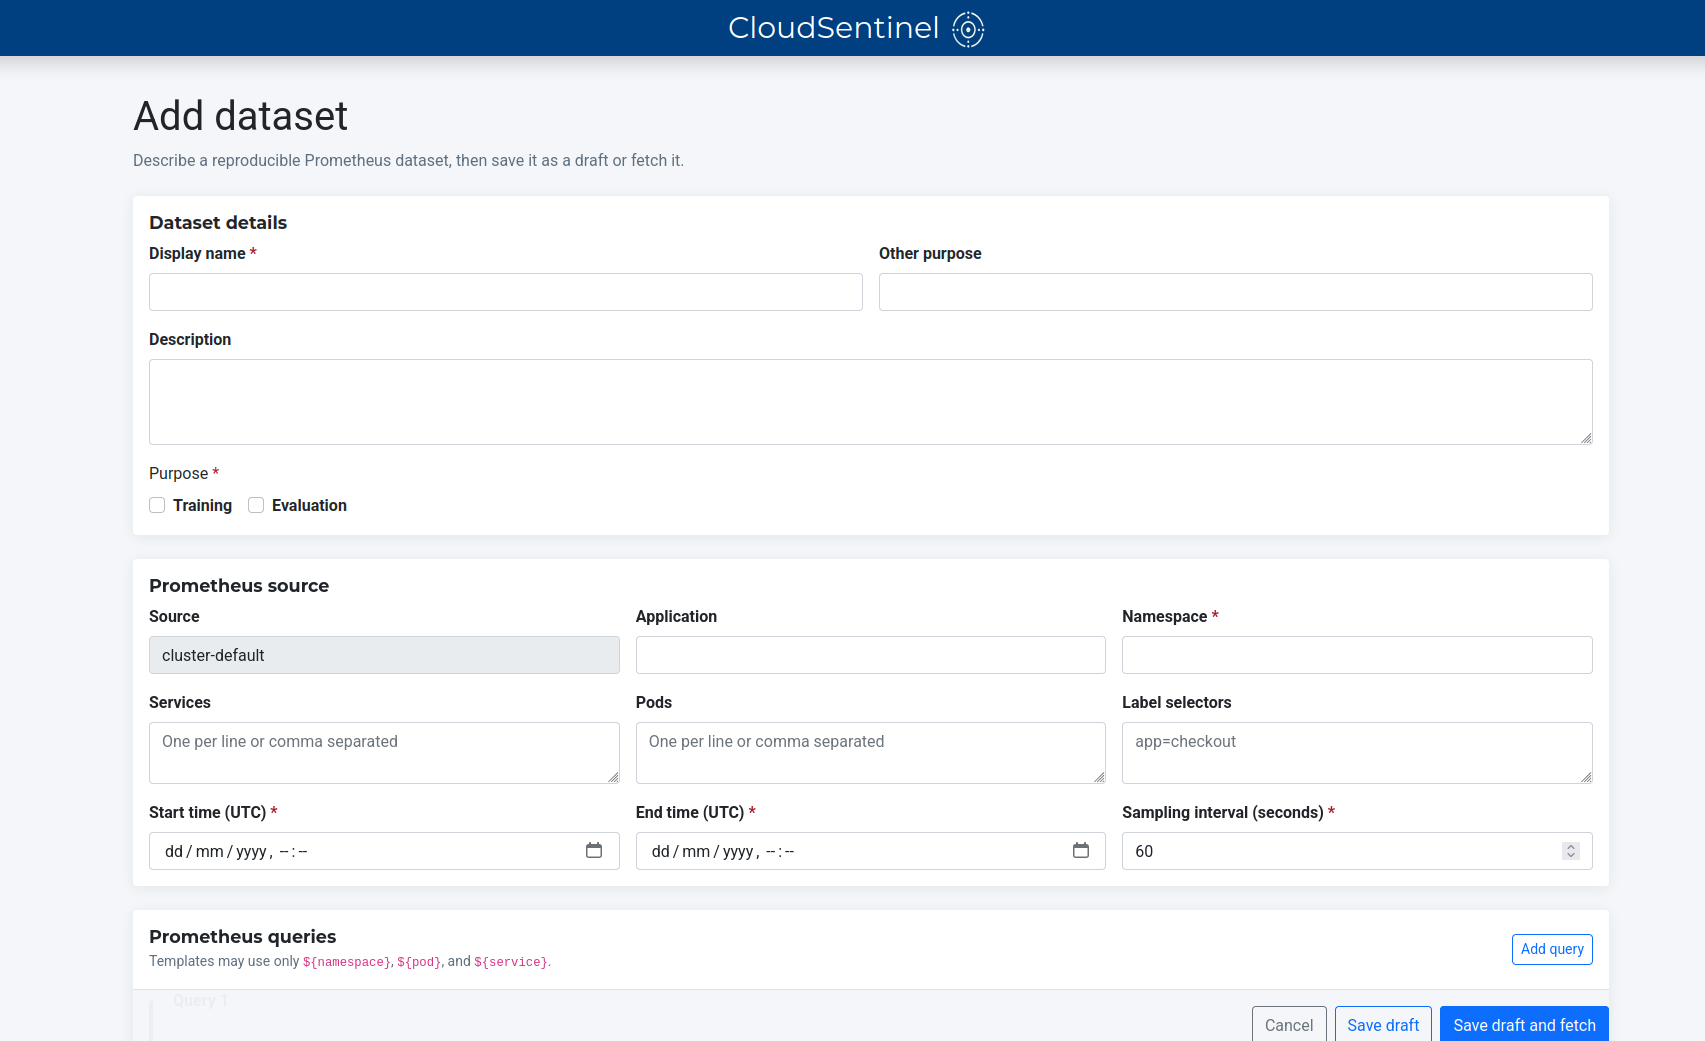
\includegraphics[width=0.9\linewidth]{figures/implementation/data_catalogue/Screenshot from 2026-10-06 17-19-07.png}
    \caption{Dataset creation form for descriptive metadata, Prometheus source selection, target selection, and the requested UTC time window.}
    \label{fig:data_catalogue_ui_add_source}
\end{figure}

\begin{figure}[H]
    \centering
    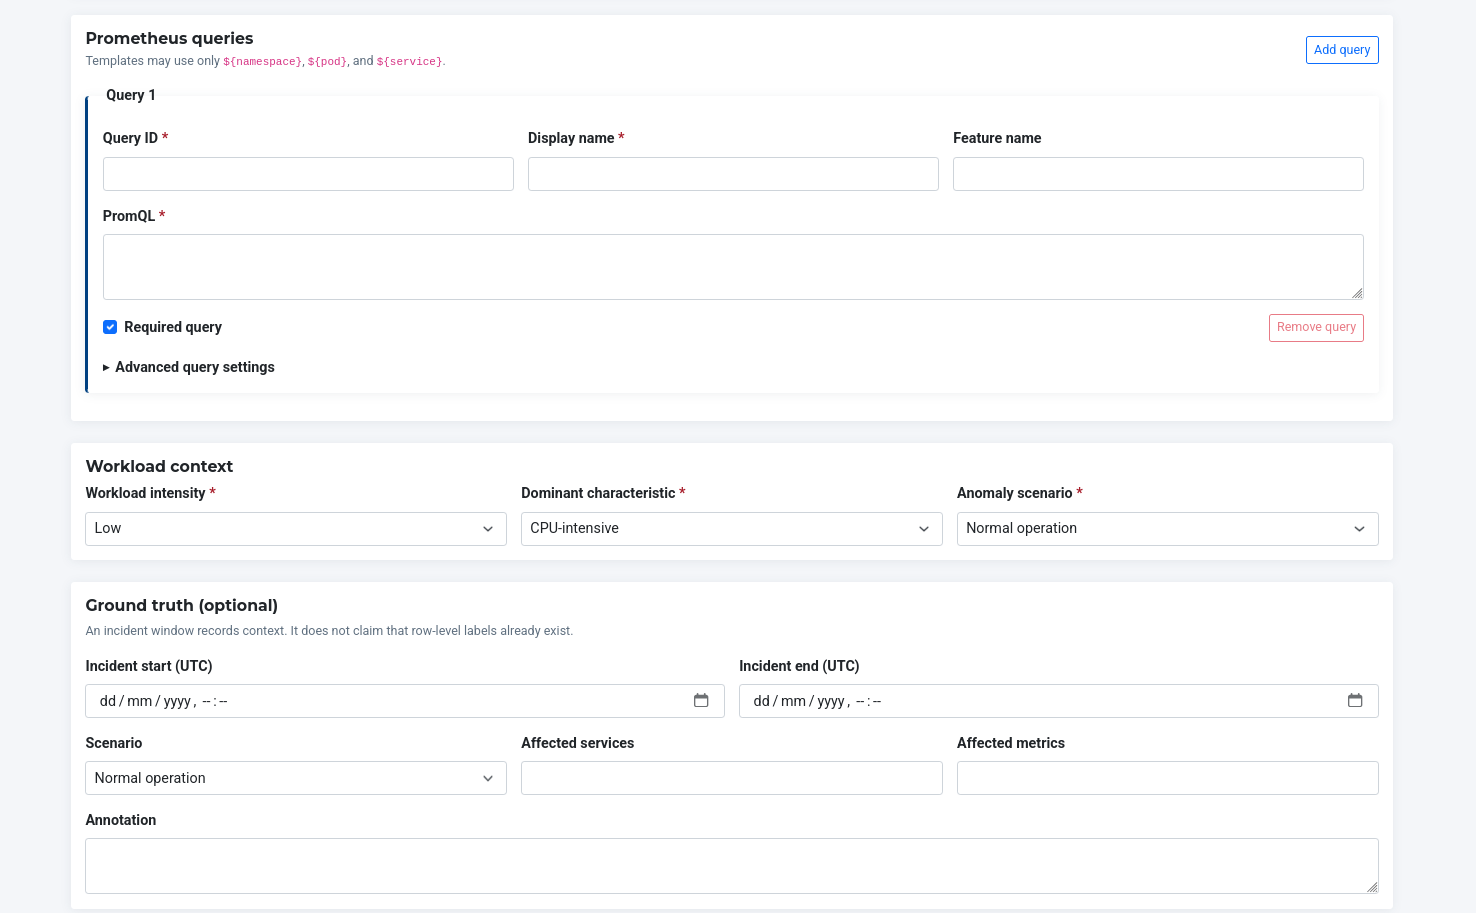
\includegraphics[width=0.9\linewidth]{figures/implementation/data_catalogue/Screenshot from 2026-10-06 17-19-27.png}
    \caption{Dataset creation form for PromQL queries, workload context, and optional incident ground truth.}
    \label{fig:data_catalogue_ui_add_context}
\end{figure}

The final part of the form, shown in Figure~\ref{fig:data_catalogue_ui_add_partition}, makes partitioning explicit. No automatic percentage split is applied. The operator either leaves the version unpartitioned or selects exact train and test intervals and an optional gap. This avoids an invisible split that might place part of a known incident in the training data. The same form offers separate actions for saving a draft and for saving and immediately starting the asynchronous fetch.

\begin{figure}[H]
    \centering
    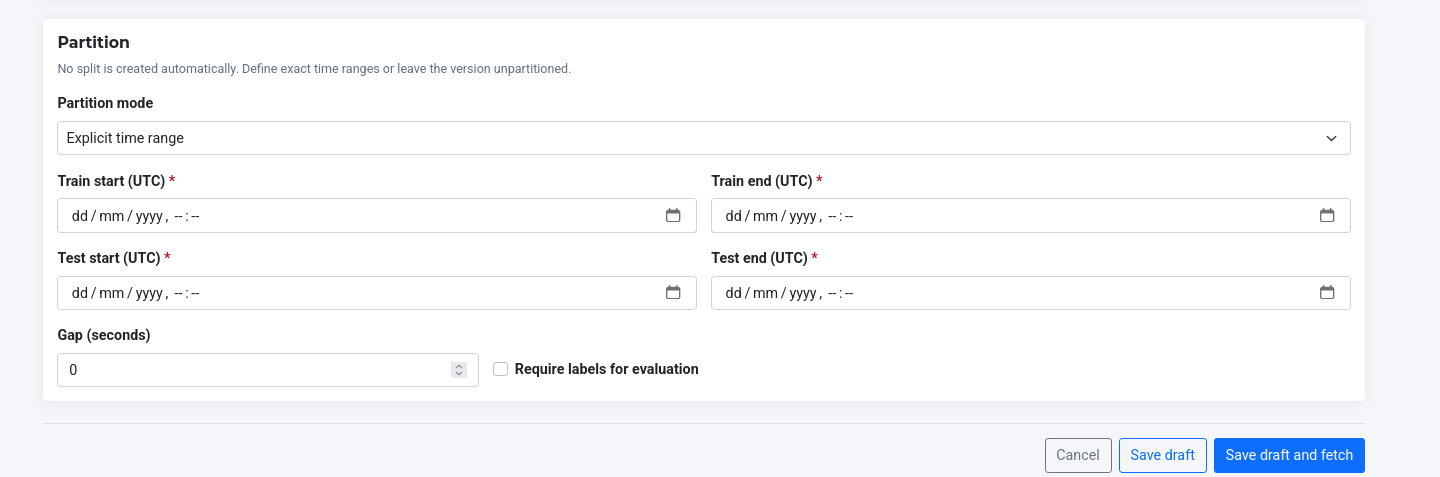
\includegraphics[width=1\linewidth]{figures/implementation/data_catalogue/Screenshot from 2026-10-06 17-19-38.png}
    \caption{Explicit time-range partition and the actions for saving a draft or starting data collection.}
    \label{fig:data_catalogue_ui_add_partition}
\end{figure}

After creation, the detail page presents the selected version, fetch progress, technical schema, recorded source and provenance, validation warnings, a bounded data preview, incidents, labels, and partition history. Actions that change interpretation, such as deriving labels or creating a partition, call dedicated API operations. Internal storage paths and credentials are removed from data passed to the browser.

\subsubsection{Additional acquisition and experiment paths}

Two additions make the catalogue usable beyond a manually chosen Prometheus window. First, a researcher can import an existing timestamped metrics file. The CSV importer in Figure~\ref{fig:data_catalogue_csv_import} checks the timestamp order, numeric feature values, optional binary labels, file size, and row count. The user maps the timestamp and label columns, records the source study and workload context, and chooses a chronological training percentage. CloudSentinel stores the original file checksum and column mapping as provenance. Imported data can be used for training and comparison, although it cannot automatically be used for live monitoring because it has no Prometheus query recipe.

\begin{figure}[H]
    \centering
    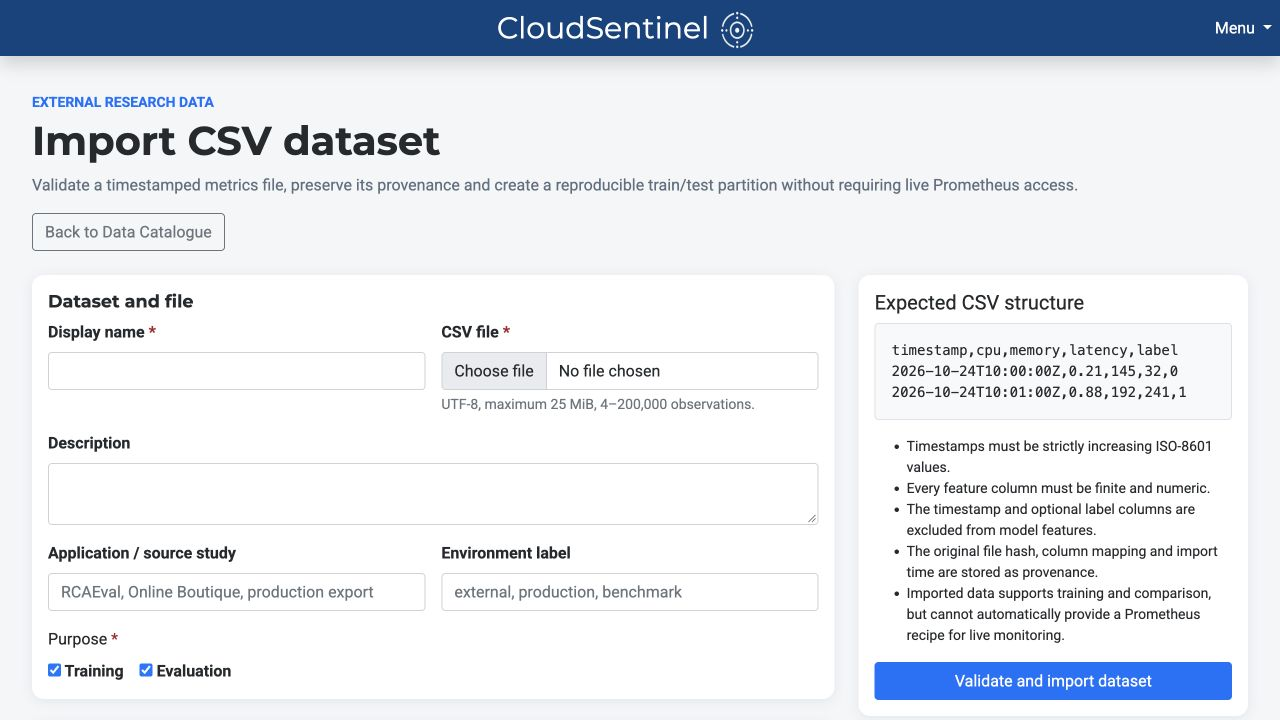
\includegraphics[width=1\linewidth]{figures/implementation/current/csv_import.jpg}
    \caption{CSV import for externally collected or benchmark data, including validation, provenance fields, and an explicit chronological partition.}
    \label{fig:data_catalogue_csv_import}
\end{figure}

Second, the controlled-workload page can create a short and bounded traffic change in the monitored Online Boutique environment. As shown in Figure~\ref{fig:controlled_workload}, the researcher selects an elevated-traffic or traffic-burst profile and a duration between two and fifteen minutes. The service records the previous load-generator settings, applies the change, restores the previous settings, and retains the actual start and end time. A completed record links directly to dataset creation with that time window and workload context already filled in. This supports repeatable experiments without presenting the feature as a general fault-injection platform.

\begin{figure}[H]
    \centering
    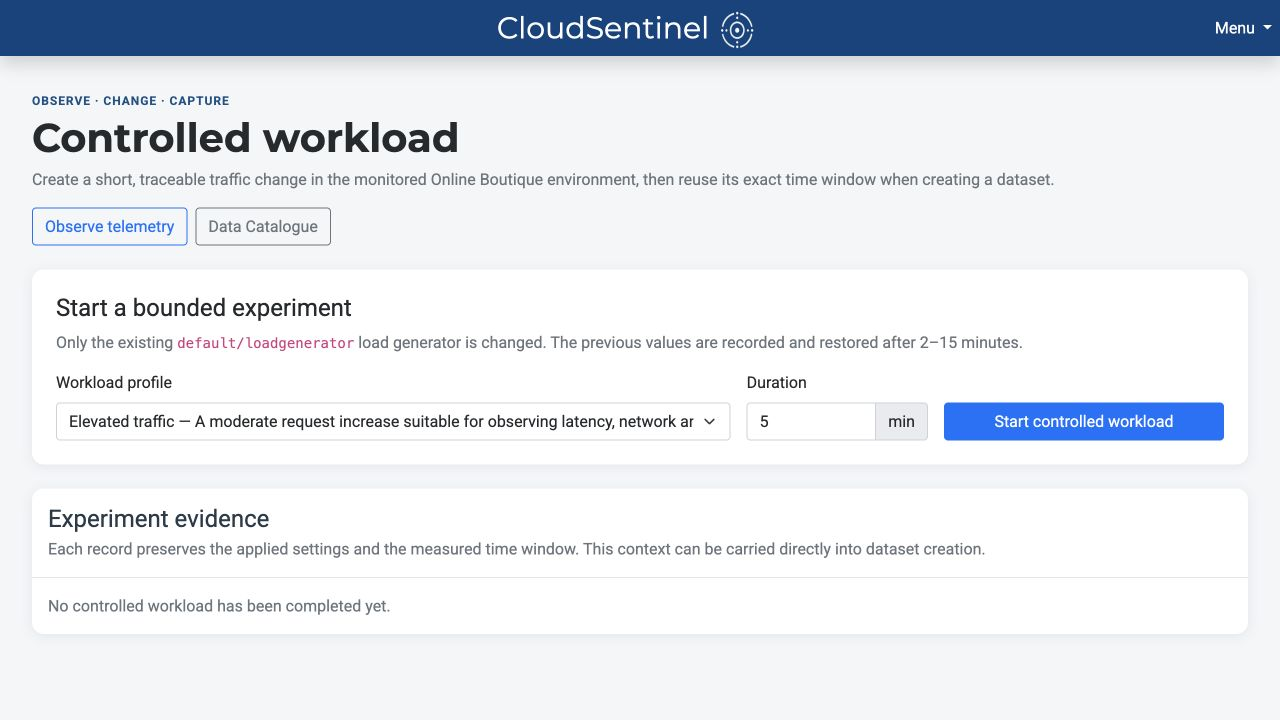
\includegraphics[width=1\linewidth]{figures/implementation/current/controlled_workload.jpg}
    \caption{Controlled-workload page for creating and recording a bounded traffic change before dataset collection.}
    \label{fig:controlled_workload}
\end{figure}

\subsubsection{Deployment and implementation boundaries}

The Kubernetes configuration mounts a 5~GiB ReadWriteOnce persistent-volume claim in both the data-ingestion API pod and its Celery worker. Both processes use the same configured catalogue storage root. The active Prometheus connection is managed through the protected monitored-environment configuration and is represented in dataset records only by the safe source identifier \texttt{cluster-default}. The containers run as a non-root user, and the fetch worker currently uses concurrency one.

These choices match the controlled, single-node staging environment used in this study, but they also define the current boundary of the implementation. The file-backed repository does not provide distributed locking and the \texttt{ReadWriteOnce} volume is not intended for independent writers on several nodes. A production deployment with multiple replicas would require shared object storage or a database, cross-process coordination, and a storage access mode suitable for multiple nodes. The health endpoints also report process health only; they do not prove that Redis, Prometheus, the worker, and the persistent volume are all functioning together.

\subsubsection{Resulting workflow}

The implemented workflow replaces a set of disconnected manual steps with one traceable process. An operator defines the monitoring context and queries, saves a draft, and starts collection. CloudSentinel then retrieves the requested time series, constructs a canonical matrix, validates the artefacts, records their checksums, and exposes their readiness. Incident context, labels, and training and test partitions can be added without changing the collected observations. Training consumes an exact, verified bundle and retains its catalogue references in the resulting run. The Data Catalogue therefore provides practical dataset management as well as the provenance needed to understand how a model's input was produced.

\subsection{Detector Models \& Training}

The detector models and training implementation provides one workflow for discovering detector implementations, selecting compatible data, training one or more detectors, and storing the resulting models. The central design choice is that detector-specific behaviour is placed behind a small plugin contract. CloudSentinel can therefore manage different detector types without adding a separate training page, API route, or worker task for every algorithm.

The term \emph{custom detector import} needs a precise meaning in this implementation. CloudSentinel accepts a detector package through the protected Add detector page, but this is not an untrusted end-user upload. A developer provides the implementation and a trusted operator authorises its publication. After validation and explicit activation, the versioned release appears in the Detector Library and can be used by the normal training workflow. Trained model files are then produced and managed by CloudSentinel itself.

\subsubsection{Implementation overview}

Figure~\ref{fig:detector_training_architecture} shows the main components. The Django user interface retrieves detector manifests, datasets, training history, and saved-model records from the learning-adaptation API. When training is started, this API verifies the selected Data Catalogue version and creates an immutable local snapshot. It then creates one parent training run with an independent child for every selected detector. Celery workers execute these children asynchronously through the detector adapters.

Detector descriptions are obtained from the detector registry. Built-in plugins are packaged with CloudSentinel, while activated external releases are discovered from the plugin repository. The Learning API has narrowly scoped write access for authorised publication; training workers and the detection runtime consume published releases. A worker loads detector code only when its child task starts. Successful training produces an artefact that is validated and atomically published to model-artifact storage. A separate Saved Model record retains safe metadata and provenance without exposing internal filesystem paths.

\begin{figure}[H]
    \centering
    \resizebox{0.98\linewidth}{!}{%
    \begin{tikzpicture}[
        font=\small,
        node distance=11mm and 11mm,
        component/.style={draw, rounded corners=2pt, align=center, minimum height=11mm, text width=28mm, fill=blue!7},
        storage/.style={draw, cylinder, shape border rotate=90, aspect=0.25, align=center, minimum height=14mm, text width=27mm, fill=green!10},
        external/.style={draw, rounded corners=2pt, align=center, minimum height=11mm, text width=27mm, fill=orange!12},
        flow/.style={-{Latex[length=2mm]}, thick},
        readonly/.style={-{Latex[length=2mm]}, thick, dashed}
    ]
        \node[component] (ui) {Django models and training interface};
        \node[component, right=of ui] (api) {Learning-adaptation API};
        \node[component, right=of api] (worker) {Generic Celery training worker};
        \node[storage, above=15mm of worker] (plugins) {Built-in and external plugin releases};
        \node[external, below=16mm of ui] (catalogue) {Data Catalogue\\verified bundle};
        \node[storage, below=16mm of worker, xshift=-18mm] (runs) {Snapshots, runs, and model records};
        \node[storage, below=16mm of worker, xshift=22mm] (artifacts) {Immutable model artefacts};

        \draw[flow] (ui) -- node[above, font=\scriptsize] {HTTP} (api);
        \draw[flow] (api) -- node[above, font=\tiny] {Redis task} (worker);
        \draw[flow] (catalogue) -- node[above left, font=\scriptsize] {verify bundle} (api);
        \draw[readonly] (plugins) -- node[right, font=\scriptsize] {pinned adapter} (worker);
        \draw[flow] (api) -- (runs);
        \draw[flow] (worker) -- (runs);
        \draw[flow] (worker) -- (artifacts);
    \end{tikzpicture}%
    }
    \caption{Implemented architecture for detector discovery, generic training, run persistence, and model publication.}
    \label{fig:detector_training_architecture}
\end{figure}

\subsubsection{Detector plugins and registry}

The registry converts detector implementations into a common public description. A detector is discovered when a direct child of a configured detector root contains a \texttt{manifest.yaml} file. The installed \texttt{detectors} Python package is scanned first and contains the built-in CGNN and Isolation Forest plugins. Additional active releases can be mounted from the external plugin repository. External plugins cannot replace a built-in detector identifier.

Discovery reads and validates manifests, but deliberately does not import the configured Python entry point. This allows the API to list detector names, capabilities, requirements, and parameters without executing detector code. Every manifest is validated independently. An invalid manifest, unsafe path, or duplicate external identifier is reported as a safe discovery error, while unrelated valid detectors remain available. Adapter code is resolved lazily when a training child actually starts.

The registry distinguishes a detector's logical identifier, release version, source, package checksum, manifest checksum, and runtime profile. These values form a plugin reference. Every training child stores this exact reference, so a queued run still loads the release that was selected when the run was created, even if an operator activates a newer release in the meantime.

\subsubsection{Custom detector package format}

A custom detector is supplied as a directory rather than as one Python file. The minimum package is shown in Figure~\ref{fig:detector_plugin_package}. The manifest describes the plugin to CloudSentinel, the adapter connects the detector-specific implementation to the shared contracts, and \texttt{requirements.lock} declares exact third-party package versions. Additional implementation modules and an optional README may be included.

\begin{figure}[H]
    \centering
    \resizebox{0.92\linewidth}{!}{%
    \begin{tikzpicture}[
        font=\small,
        node distance=9mm and 12mm,
        root/.style={draw, rounded corners=2pt, align=center, minimum height=10mm, text width=30mm, fill=blue!10},
        required/.style={draw, rounded corners=2pt, align=left, minimum height=13mm, text width=39mm, fill=green!9},
        optional/.style={draw, rounded corners=2pt, align=left, minimum height=13mm, text width=39mm, fill=gray!10},
        link/.style={-{Latex[length=2mm]}, thick}
    ]
        \node[root] (root) {\texttt{my\_detector/}};
        \node[required, below left=of root, xshift=-18mm] (manifest) {\textbf{\texttt{manifest.yaml}}\\identity, capabilities, input requirements, parameters, entry point};
        \node[required, below=of root] (adapter) {\textbf{\texttt{adapter.py}}\\validation, preprocessing, training, evaluation, artefact result};
        \node[required, below right=of root, xshift=18mm] (requirements) {\textbf{\texttt{requirements.lock}}\\exact versions already present in the selected runtime};
        \node[optional, below=17mm of adapter] (extra) {\textbf{Optional files}\\implementation modules and documentation};

        \draw[link] (root) -- (manifest);
        \draw[link] (root) -- (adapter);
        \draw[link] (root) -- (requirements);
        \draw[link] (adapter) -- (extra);
    \end{tikzpicture}%
    }
    \caption{Minimum external detector package and the responsibility of each supplied file.}
    \label{fig:detector_plugin_package}
\end{figure}

Imports between plugin modules must be relative to the plugin package, for example \texttt{from .implementation import train\_model}. The manifest entry point is also plugin-relative, such as \texttt{adapter:MyDetectorAdapter}. The publication process rejects symlinks, virtual environments, Git metadata, bytecode, sockets, and other special files. This keeps the published release small and prevents package paths from escaping their assigned repository directory.

The dependency lock file is a compatibility declaration, not an installation instruction. A line such as \texttt{numpy==1.26.4} states that the plugin expects that exact version to exist in its selected runtime profile. CloudSentinel never runs \texttt{pip install} while publishing or training a plugin. A missing or incompatible dependency therefore stops publication rather than changing the shared worker environment.

\subsubsection{Detector manifest}

The manifest is the stable contract between a detector and the rest of CloudSentinel. Schema version~1 requires a schema version, unique identifier, display name, plugin version, description, supported modalities, capabilities, input requirements, training parameters, and an entry point. An external plugin can also select a supported runtime profile; otherwise the current CPU Python machine-learning profile is used.

The training capability states whether training is enabled and identifies both the protocol and expected input profile. The current generic combination is \texttt{cloudsentinel.training/v1} with \texttt{metrics-partition-v1}. The latter represents checksummed training, test, and label CSV files with dataset and feature provenance. Inference is optional. When enabled, the manifest also declares the inference protocol, input profile, and artefact format.

\begin{verbatim}
schema_version: 1
id: my-detector
name: My detector
version: 1.0.0
supported_modalities: [metrics]
capabilities:
  training:
    enabled: true
    protocol: cloudsentinel.training/v1
    input_profile: metrics-partition-v1
training_parameters: {}
entry_point: adapter:MyDetectorAdapter
\end{verbatim}

Each training parameter declares a type, default value, and user-facing description. Supported types are Boolean, integer, number, and string. Optional constraints include inclusive or exclusive minimum and maximum values, allowed or excluded values, nullability, and whether a parameter is advanced. The registry verifies that defaults match these constraints. Unknown submitted parameters are rejected instead of being forwarded to the adapter. Relationships that depend on a particular dataset, such as requiring \texttt{n\_neighbors} to be smaller than the number of training rows, cannot be expressed by a simple manifest bound and are checked by the adapter.

This manifest information has two uses. The backend applies it as a validation schema, while the user interface uses the same data to display detector capabilities and generate correctly typed parameter fields. A new compatible plugin can therefore appear in the existing interface without a detector-specific frontend change.

\subsubsection{Adapter contract and responsibility boundary}

Every trainable adapter implements two methods. \texttt{validate\_training()} checks detector-specific compatibility using the supplied training context. \texttt{run\_training()} performs preprocessing, fitting, evaluation, and artefact creation. It reports bounded progress and returns a common \texttt{TrainingResult}. If inference is enabled, the same adapter also implements methods for loading its saved artefact and producing predictions under the generic inference contract.

The training context contains the verified train, test, and label paths; observation and feature counts; the fixed feature identity; validated parameters; dataset and snapshot provenance; logical run and model identifiers; and a private artefact workspace. An adapter may only write below this workspace. It returns the directory, required filenames, artefact format, compact evaluation results, and bounded model metadata. It never returns public server paths.

This creates a clear boundary. The adapter owns detector-specific data checks, preprocessing, model fitting, evaluation, and the contents of its model artefact. The generic executor owns lifecycle persistence, progress states, failure handling, validation of returned files, immutable artefact publication, and creation of the Saved Model record. Consequently, a detector developer does not have to implement CloudSentinel's orchestration and storage logic again.

\subsubsection{Installing, activating, and versioning external detectors}

External plugins are treated as trusted server-side code and are published by a trusted operator, not by an ordinary browser user. The normal publication command accepts an absolute path to a plugin directory together with assertions for its detector identifier and version. A wrapper creates a temporary Kubernetes administration pod, copies the package to private staging, performs validation, installs an immutable release, optionally activates it, and removes both the staging copy and the temporary pod.

Figure~\ref{fig:detector_plugin_lifecycle} shows this lifecycle. Validation covers the package layout, safe files and paths, manifest schema, dependency pins, adapter import, and required adapter methods. Installation calculates deterministic SHA-256 hashes and publishes the package below its detector identifier, version, and content digest. Installation alone does not change the active release. Activation is an explicit atomic switch, which makes it possible to inspect a release before making it available to new runs.

\begin{figure}[H]
    \centering
    \resizebox{0.98\linewidth}{!}{%
    \begin{tikzpicture}[
        font=\small,
        node distance=8mm,
        state/.style={draw, rounded corners=2pt, align=center, minimum height=11mm, text width=27mm, fill=blue!7},
        stored/.style={draw, rounded corners=2pt, align=center, minimum height=11mm, text width=27mm, fill=green!10},
        fail/.style={draw, rounded corners=2pt, align=center, minimum height=11mm, text width=26mm, fill=red!8},
        flow/.style={-{Latex[length=2mm]}, thick}
    ]
        \node[state] (source) {Plugin source directory};
        \node[state, right=of source] (staging) {Private staging copy};
        \node[state, right=of staging] (validation) {Package and contract validation};
        \node[stored, right=of validation] (release) {Immutable installed release};
        \node[stored, right=of release] (active) {Active reference for future runs};
        \node[fail, below=12mm of validation] (reject) {Rejected; previous active release unchanged};

        \draw[flow] (source) -- (staging);
        \draw[flow] (staging) -- (validation);
        \draw[flow] (validation) -- node[above, font=\scriptsize] {valid} (release);
        \draw[flow] (validation) -- node[right, font=\scriptsize] {invalid} (reject);
        \draw[flow] (release) -- node[above, font=\scriptsize] {activate} (active);
        \draw[flow] (active.south) to[bend left=24] node[below, font=\scriptsize] {rollback} (release.south);
    \end{tikzpicture}%
    }
    \caption{External detector publication separates validation, immutable installation, activation, and rollback.}
    \label{fig:detector_plugin_lifecycle}
\end{figure}

A published version is immutable. Changed code must receive a new version instead of replacing the bytes of an existing release. Rollback only changes the active reference to an older installed version. Existing queued, running, and completed runs retain their pinned release and hashes, and releases are not automatically removed while they may still be referenced.

\subsubsection{Detector and model management interface}

The Models page brings detector discovery, trained models, and training history together. The Detector Library in Figure~\ref{fig:detector_library} is generated from the validated public manifests. Each card shows the detector identity, modality, input profile, training availability, input summary, and number of parameters. Built-in and external detectors use the same presentation and the same action for starting a training workflow.

\begin{figure}[H]
    \centering
    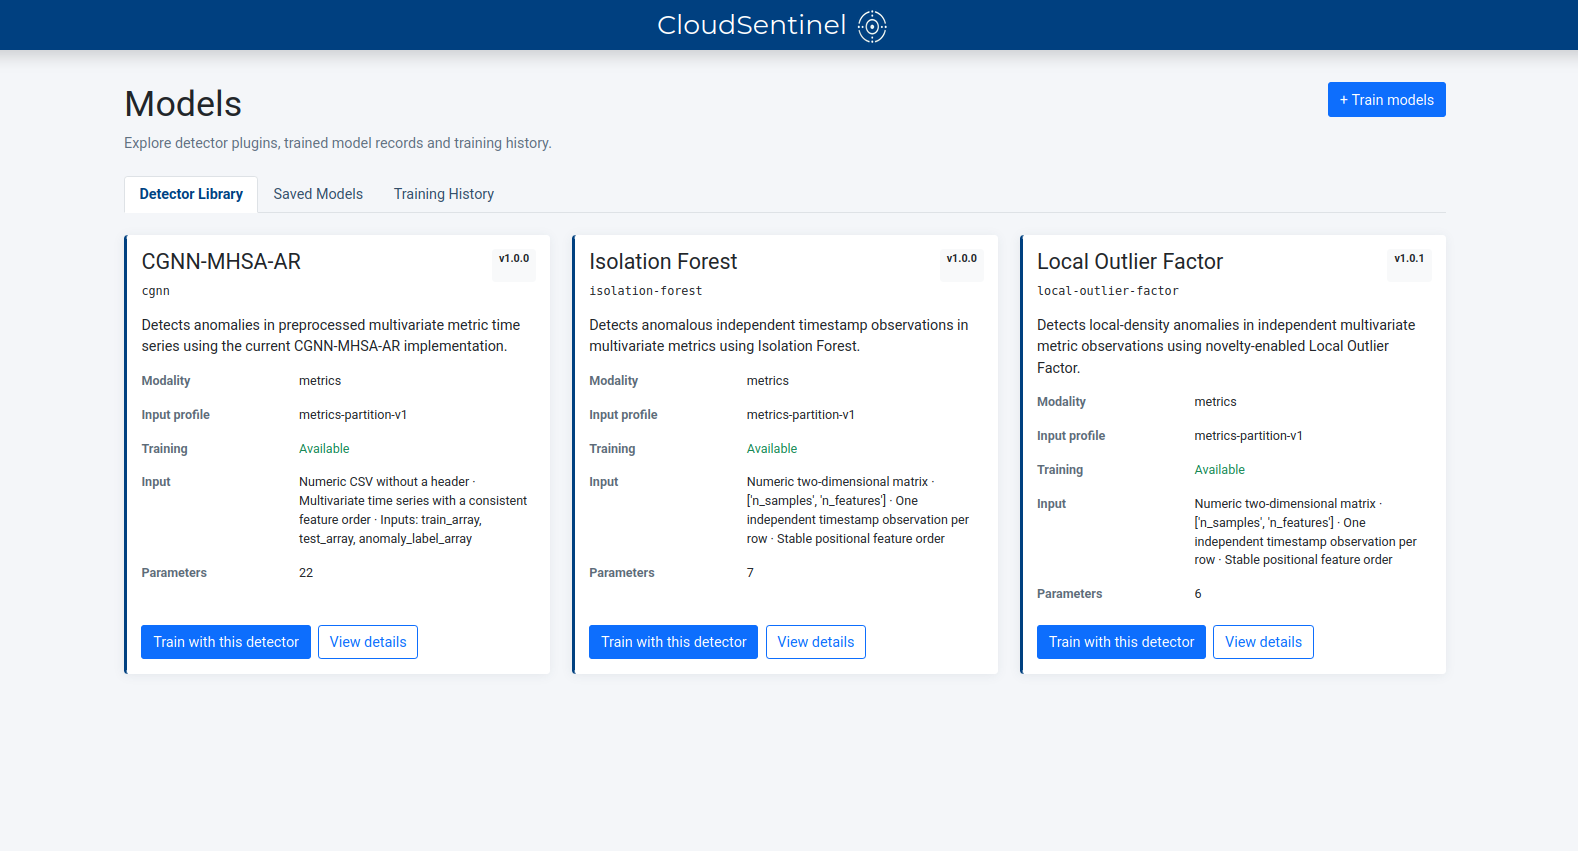
\includegraphics[width=1\linewidth]{figures/implementation/Models_and_training/Screenshot from 2026-10-06 17-24-06.png}
    \caption{Detector Library containing built-in and activated external detector plugins described by their manifests.}
    \label{fig:detector_library}
\end{figure}

The detail page in Figure~\ref{fig:detector_detail} shows how the manifest is translated into operator-facing information. It presents capabilities and input requirements together with parameter types, defaults, constraints, and descriptions. Advanced parameters are collapsed by default so the most commonly changed values remain visible without hiding the full configuration.

\begin{figure}[H]
    \centering
    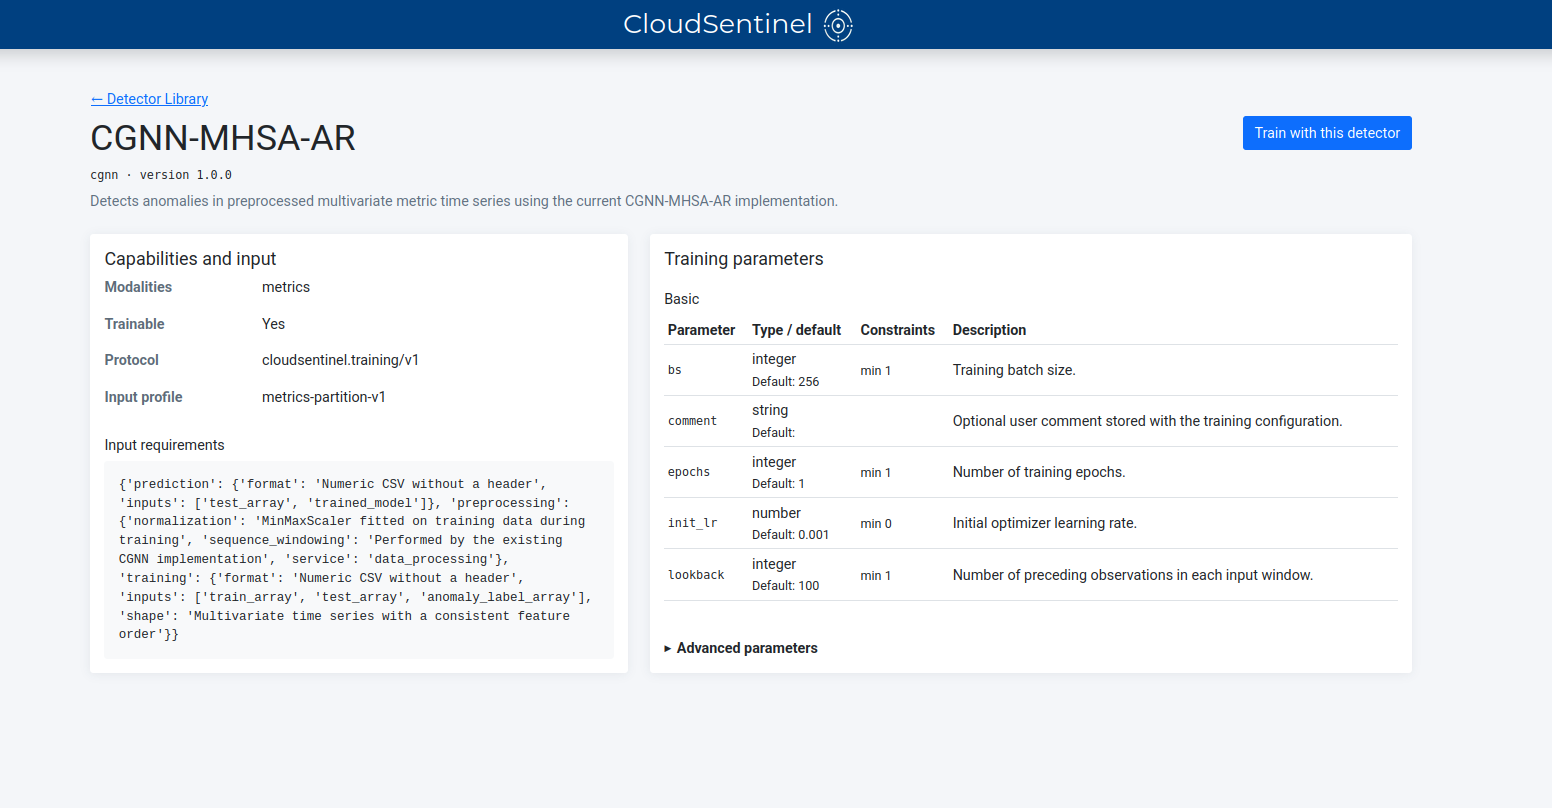
\includegraphics[width=1\linewidth]{figures/implementation/Models_and_training/Screenshot from 2026-10-06 17-25-06.png}
    \caption{Detector detail page generated from the CGNN manifest, including capabilities and validated training parameters.}
    \label{fig:detector_detail}
\end{figure}

The Saved Models tab, shown in Figure~\ref{fig:saved_models_overview}, lists only models for which training and artefact publication succeeded. Records can be filtered by detector, status, or dataset. Every row links back to the source dataset and training run, which makes the model catalogue a provenance index rather than only a directory of binary files.

\begin{figure}[H]
    \centering
    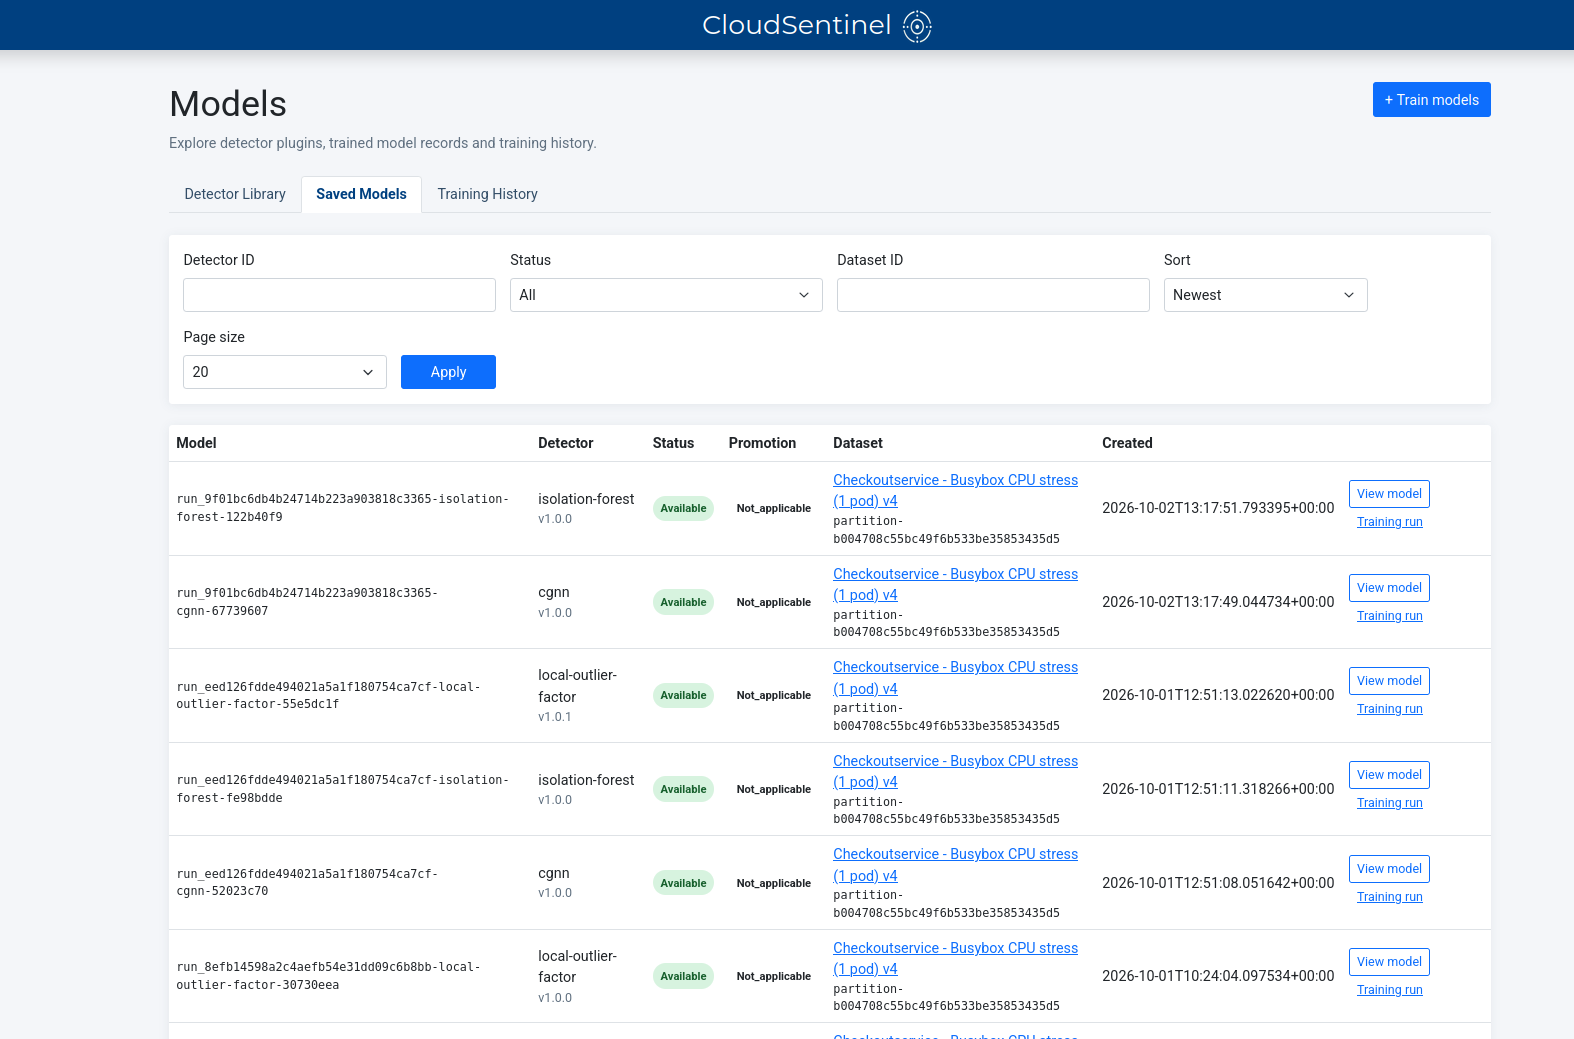
\includegraphics[width=1\linewidth]{figures/implementation/Models_and_training/Screenshot from 2026-10-06 17-25-20.png}
    \caption{Saved Models overview with detector, availability, dataset provenance, and links to the originating training run.}
    \label{fig:saved_models_overview}
\end{figure}

The Training History tab in Figure~\ref{fig:training_history_overview} lists parent runs and their detector children. It supports filters for lifecycle state, detector, dataset, and dataset source. The interface also shows partial success: one detector may fail while another detector trained from the same snapshot still produces a saved model.

\begin{figure}[H]
    \centering
    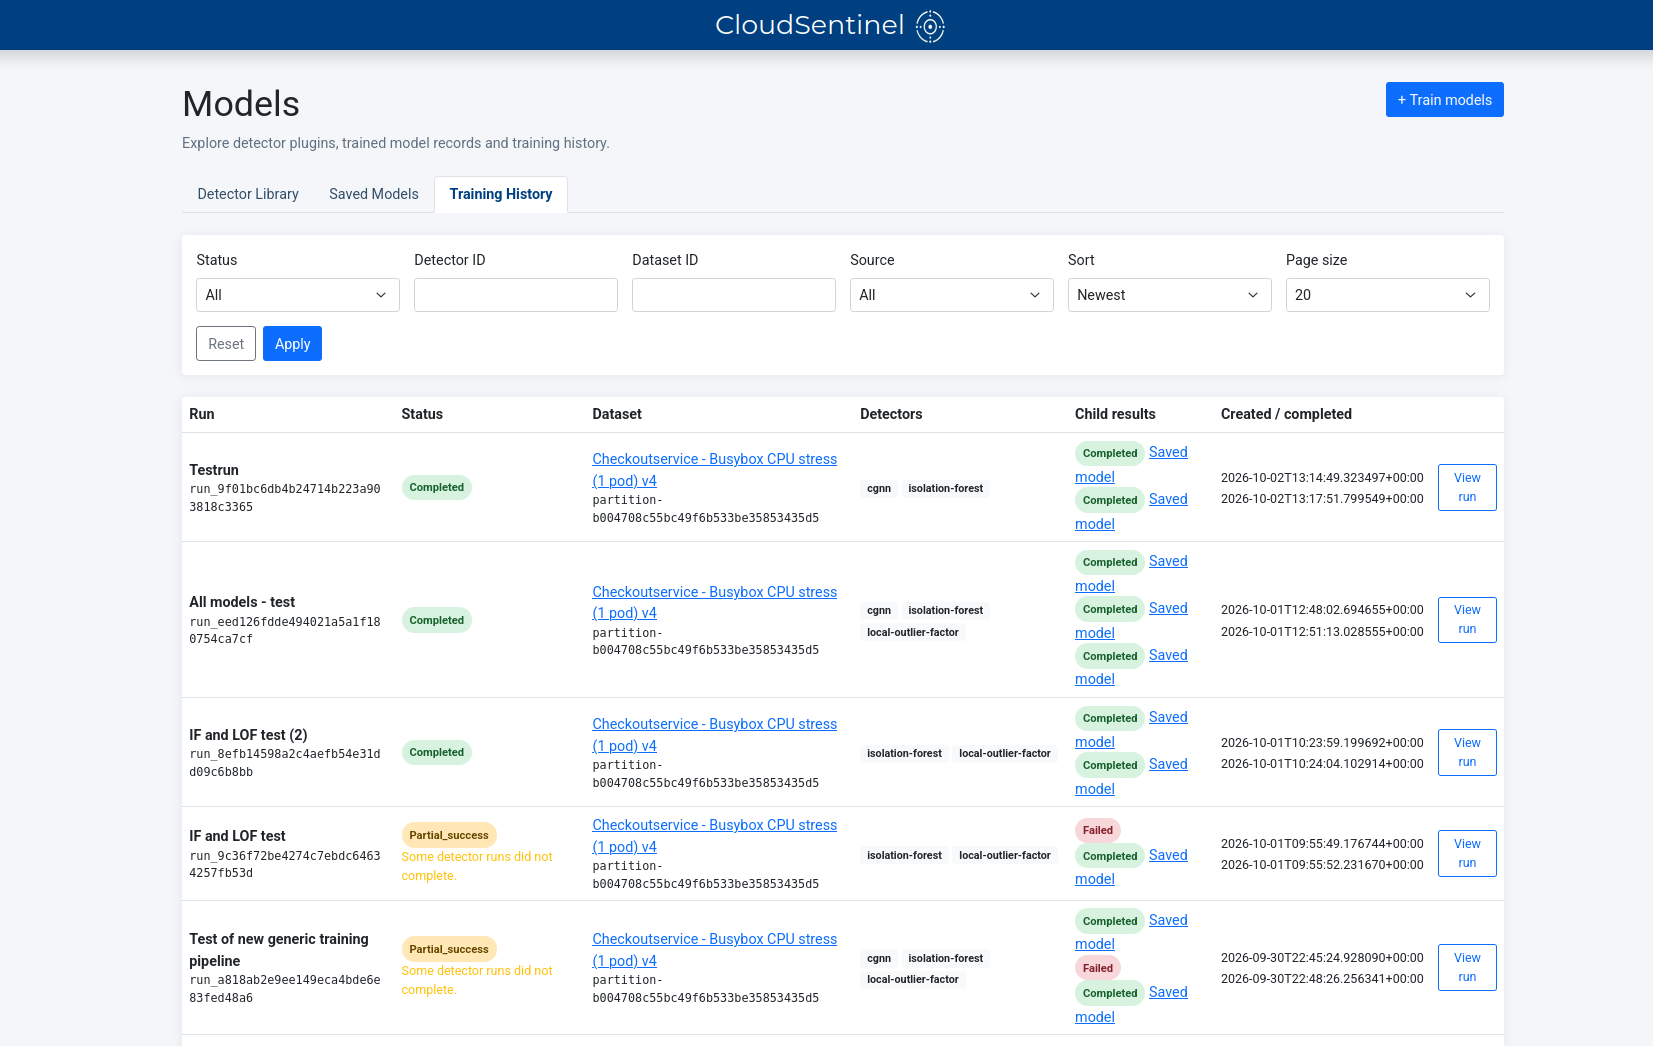
\includegraphics[width=1\linewidth]{figures/implementation/Models_and_training/Screenshot from 2026-10-06 17-25-43.png}
    \caption{Training History with parent status, selected detectors, child results, and links to successfully saved models.}
    \label{fig:training_history_overview}
\end{figure}

\subsubsection{Creating an immutable training input}

Training starts from one exact Data Catalogue dataset, version, and partition. The learning-adaptation service requests the materialised bundle described in the preceding section and verifies its manifest, identities, allowed filenames, byte limits, and SHA-256 hashes. It also checks that the train and test matrices are rectangular, have the expected feature count, and that the label file covers the test observations.

After verification, the bundle is copied atomically into an immutable snapshot. This snapshot contains \texttt{train.csv}, \texttt{test.csv}, \texttt{labels.csv}, and metadata. The metadata pins the dataset identifier and version, partition identifier and checksum, feature order and its hash, label source, observation counts, and aggregate content hash. All detector children in the same parent run read this shared snapshot; they do not make detector-specific copies of the input.

Snapshot creation happens before tasks are dispatched. A missing dataset, unavailable partition, identity mismatch, damaged archive, or checksum error therefore stops the entire request before any detector starts. Detector-specific incompatibility is handled later and only affects the corresponding child.

\subsubsection{Preprocessing and detector-specific input handling}

The Data Catalogue stores canonical observations and intentionally performs no detector-specific scaling, imputation, or sequence windowing. These operations belong to the adapter because different algorithms make different assumptions. The common requirement is that train and test data retain the same stable feature order. Any fitted preprocessing object needed later for inference is saved as part of the model artefact.

\begin{table}[H]
    \centering
    \caption{Preprocessing and input handling of the implemented detector adapters.}
    \label{tab:detector_preprocessing}
    \resizebox{\linewidth}{!}{%
    \begin{tabular}{@{}p{27mm}p{48mm}p{45mm}p{42mm}@{}}
        \toprule
        \textbf{Detector} & \textbf{Input interpretation} & \textbf{Preprocessing during training} & \textbf{Persisted preprocessing} \\
        \midrule
        CGNN-MHSA-AR & Ordered multivariate time series & Replace missing numeric values with zero; fit a MinMax scaler on training data; transform train and test; construct lookback windows & Fitted scaler together with model configuration and state dictionary \\
        Isolation Forest & One independent timestamp observation per row & Require finite numeric matrices; fit a StandardScaler and Isolation Forest pipeline on training observations & Complete scikit-learn pipeline \\
        Local Outlier Factor & One independent timestamp observation per row for novelty detection & Require finite numeric matrices; fit a StandardScaler and novelty-enabled Local Outlier Factor pipeline & Complete scikit-learn pipeline \\
        \bottomrule
    \end{tabular}%
    }
\end{table}

For CGNN, the scaler is fitted only on the training matrix and then applied to both train and test data. This avoids using test-set ranges to prepare the training input. The existing CGNN implementation subsequently creates overlapping sequences according to the configured lookback. The first lookback observations cannot receive a normal forecast in later inference and are therefore treated as warm-up observations. Feature-importance calculation is disabled for arbitrary catalogue features because their PromQL names do not provide the older implementation with a trustworthy container-by-metric mapping.

Isolation Forest and Local Outlier Factor do not use sequence windows. Each row is treated as an independent multivariate observation. Both adapters reject non-finite input rather than silently inventing values. Their standardisation and estimator are stored together in one pipeline, which ensures that inference applies exactly the transformation fitted during training. Labels are not used to fit these unsupervised estimators, but the current shared training profile requires labels because the adapters evaluate the fitted models before publishing them.

\subsubsection{Configuring and starting a training run}

The user interface divides training into four explicit steps. In the first step, shown in Figure~\ref{fig:training_select_dataset}, the user selects a dataset and exact version. Only datasets that may satisfy the current labelled partition profile are offered. Continuing causes the backend to retrieve and validate the exact version rather than trusting the summary displayed by the browser.

\begin{figure}[H]
    \centering
    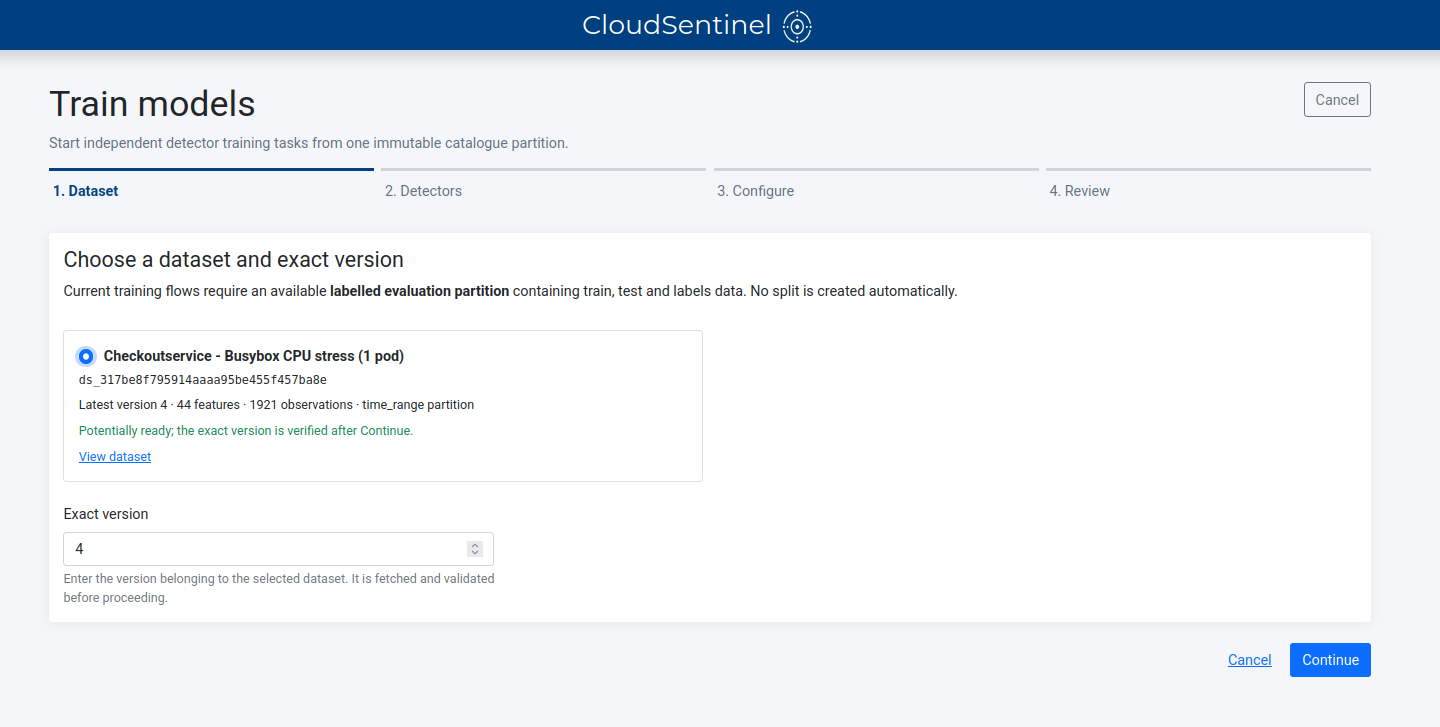
\includegraphics[width=1\linewidth]{figures/implementation/Models_and_training/training_workflow/Screenshot from 2026-10-06 17-34-06.png}
    \caption{Step 1 of the training wizard: selecting a catalogue dataset and exact immutable version.}
    \label{fig:training_select_dataset}
\end{figure}

In the second step, Figure~\ref{fig:training_select_detectors}, the interface shows the verified partition, train and test sizes, feature count, and label source. It then lists detectors whose modality and input profile match the dataset. Multiple detectors can be selected. This creates a controlled comparison point because every selected detector receives the same snapshot and feature order.

\begin{figure}[H]
    \centering
    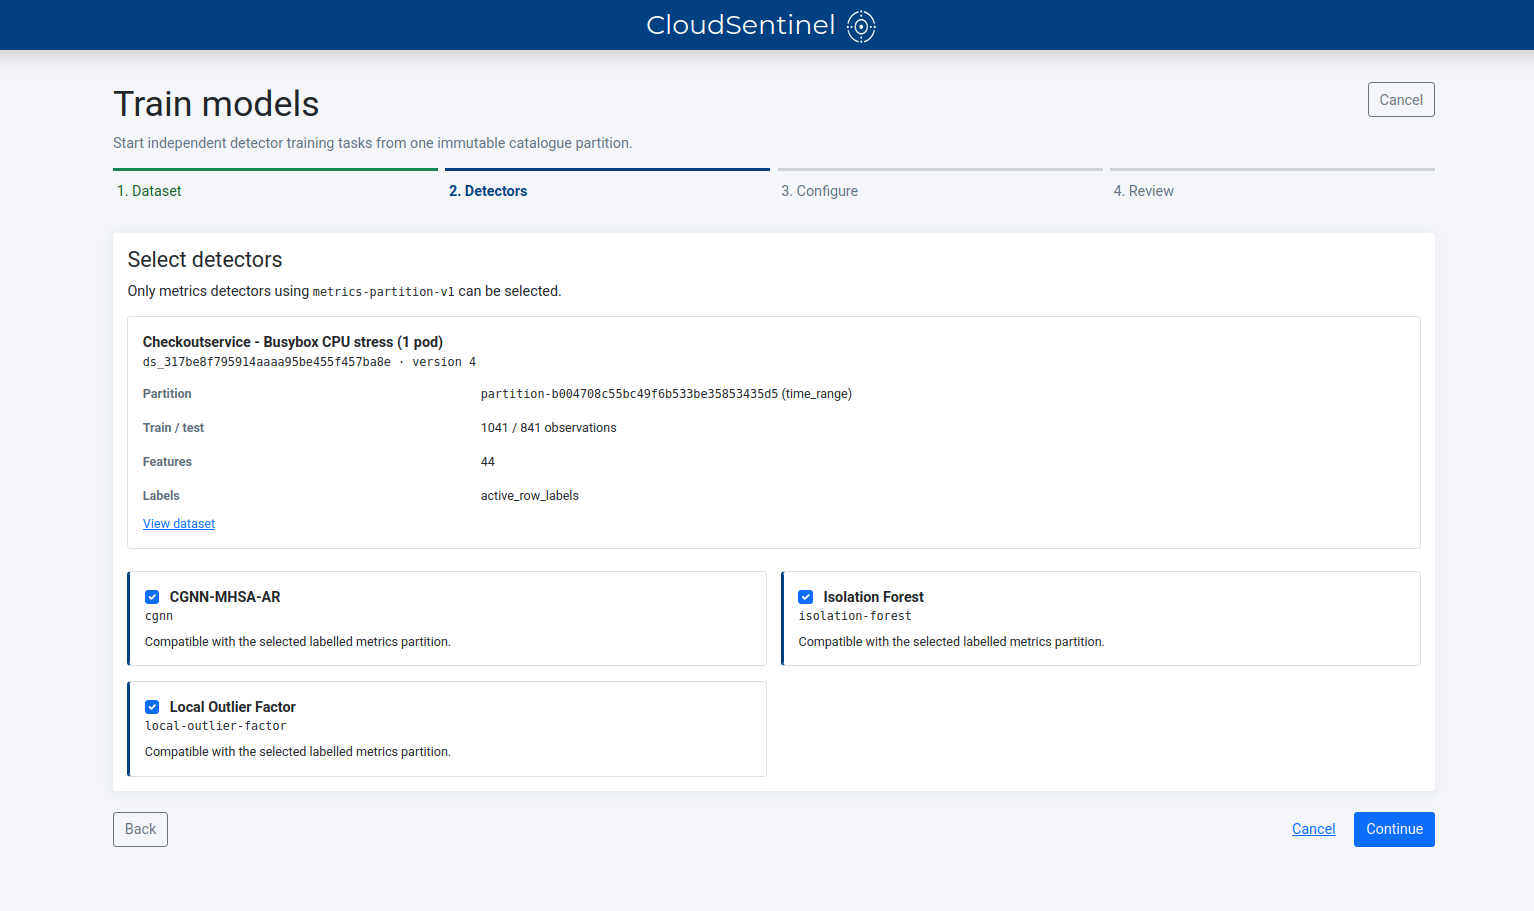
\includegraphics[width=1\linewidth]{figures/implementation/Models_and_training/training_workflow/Screenshot from 2026-10-06 17-34-40.png}
    \caption{Step 2: selecting compatible detector plugins for one verified dataset partition.}
    \label{fig:training_select_detectors}
\end{figure}

The configuration page in Figure~\ref{fig:training_configure_detectors} is generated from the selected manifests. Values receive an appropriate checkbox, number field, text field, or allowed-value selector. Basic and advanced parameters are separated. The browser uses defaults and constraints to guide the user, but the Learning API repeats type and constraint validation before creating a run. Client-side form controls are therefore not treated as a security boundary.

\begin{figure}[H]
    \centering
    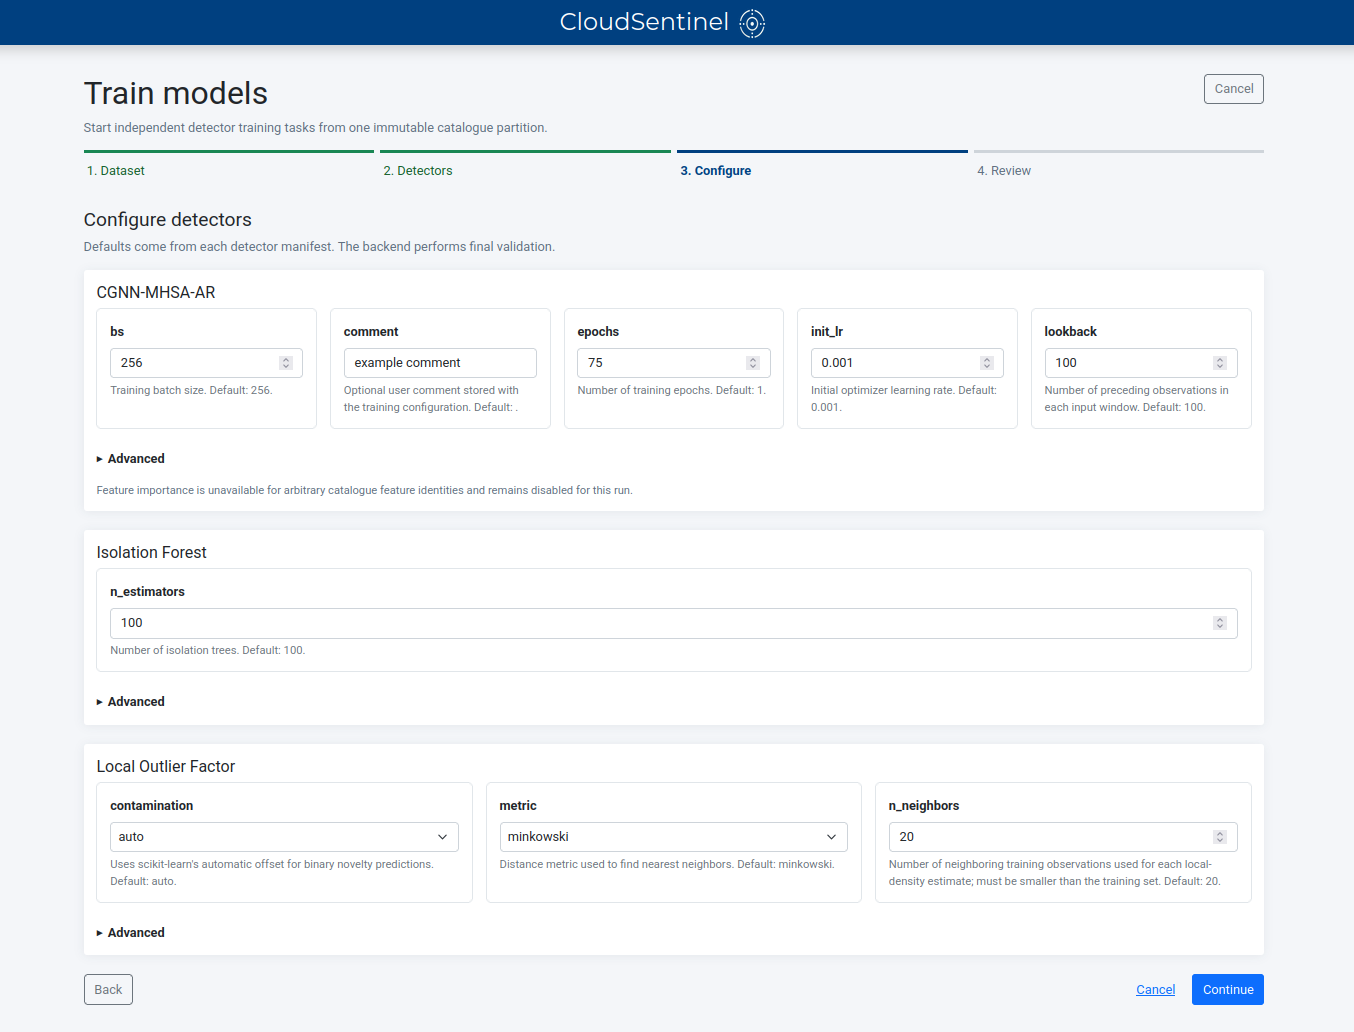
\includegraphics[width=0.95\linewidth]{figures/implementation/Models_and_training/training_workflow/Screenshot from 2026-10-06 17-35-15.png}
    \caption{Step 3: detector-specific parameter forms generated from manifest defaults, types, descriptions, and constraints.}
    \label{fig:training_configure_detectors}
\end{figure}

The review page in Figure~\ref{fig:training_review} presents the dataset identity, partition checksum, feature-order hash, label source, workload context, feature order, and complete parameter set for each detector. No automatic data split or hidden parameter change is made at this stage. Submitting the review creates one named parent run and its detector children.

\begin{figure}[H]
    \centering
    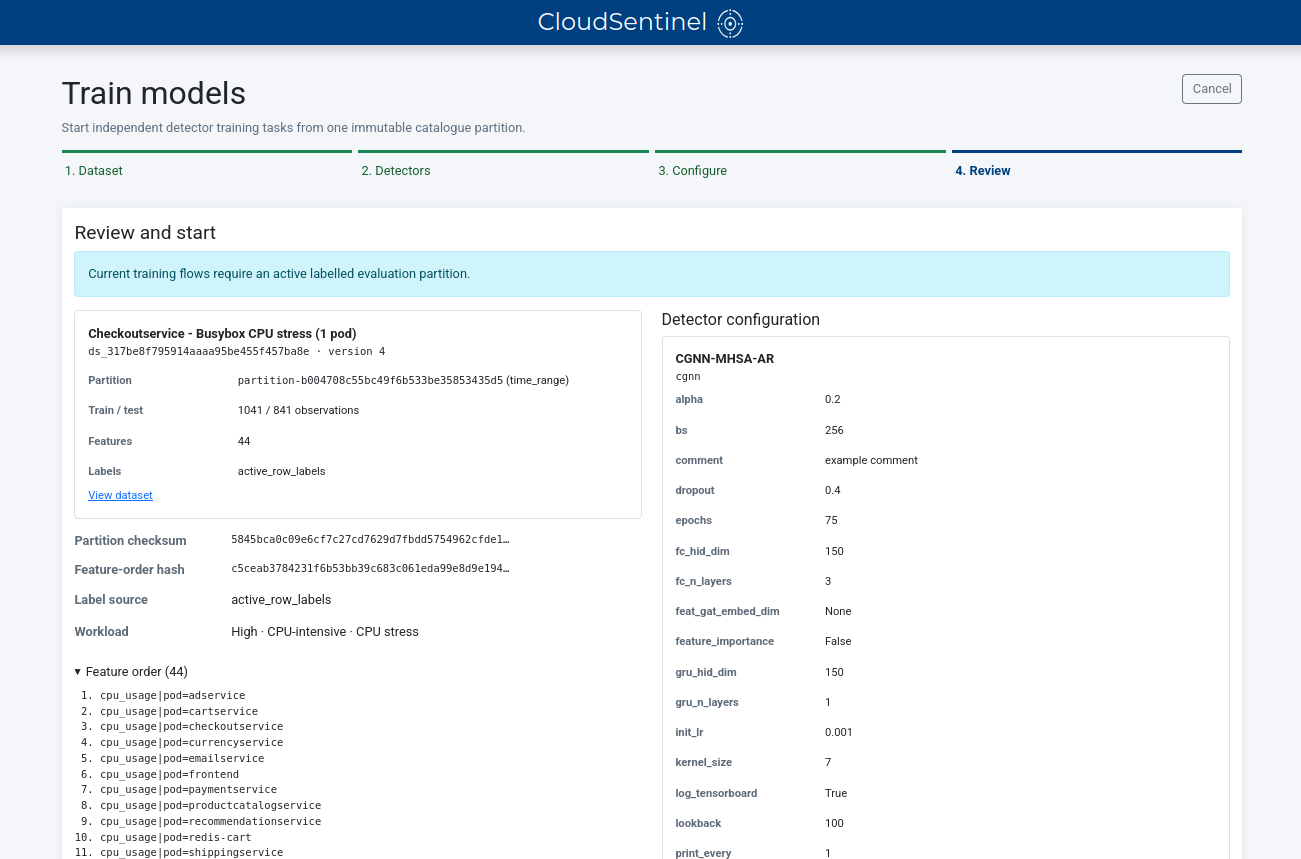
\includegraphics[width=0.95\linewidth]{figures/implementation/Models_and_training/training_workflow/Screenshot from 2026-10-06 17-35-49.png}
    \caption{Step 4: reviewing exact dataset provenance, feature identity, and detector configurations before dispatch.}
    \label{fig:training_review}
\end{figure}

\subsubsection{Generic multi-detector training pipeline}

Figure~\ref{fig:generic_training_pipeline} summarises the server-side pipeline. The API first validates the request, resolves each active detector to an exact plugin reference, and creates or reuses the immutable dataset snapshot. It persists the parent and all children before dispatch. Each child receives its own logical model identifier, parameters, and pinned plugin reference, but shares the same snapshot identity.

The worker verifies the snapshot again before use, resolves the pinned adapter, constructs a training context, and calls detector-specific validation. A compatibility error marks that child as a validation failure. A compatible adapter then preprocesses the snapshot data, fits the model, evaluates it, and returns a declared artefact. The executor validates and publishes that artefact before creating a Saved Model record. Failure in one child does not cancel its siblings.

\begin{figure}[H]
    \centering
    \resizebox{0.98\linewidth}{!}{%
    \begin{tikzpicture}[
        font=\small,
        node distance=8mm,
        pipelineStep/.style={draw, rounded corners=2pt, align=center, minimum height=11mm, text width=26mm, fill=blue!7},
        detector/.style={draw, rounded corners=2pt, align=center, minimum height=11mm, text width=28mm, fill=orange!10},
        output/.style={draw, rounded corners=2pt, align=center, minimum height=11mm, text width=27mm, fill=green!10},
        flow/.style={-{Latex[length=2mm]}, thick}
    ]
        \node[pipelineStep] (request) {Validated training request};
        \node[pipelineStep, right=of request] (snapshot) {Verified immutable snapshot};
        \node[pipelineStep, right=of snapshot] (parent) {Persist parent and detector children};
        \node[detector, below=14mm of parent, xshift=-36mm] (childa) {Child A\\validate, preprocess, train, evaluate};
        \node[detector, below=14mm of parent] (childb) {Child B\\validate, preprocess, train, evaluate};
        \node[detector, below=14mm of parent, xshift=36mm] (childc) {Child C\\validate, preprocess, train, evaluate};
        \node[output, below=16mm of childb, xshift=-24mm] (artifact) {Validate and publish immutable artefact};
        \node[output, below=16mm of childb, xshift=24mm] (model) {Create Saved Model and update run};

        \draw[flow] (request) -- (snapshot);
        \draw[flow] (snapshot) -- (parent);
        \draw[flow] (parent) -- (childa);
        \draw[flow] (parent) -- (childb);
        \draw[flow] (parent) -- (childc);
        \draw[flow] (childa) -- (artifact);
        \draw[flow] (childb) -- (artifact);
        \draw[flow] (childc) -- (artifact);
        \draw[flow] (artifact) -- (model);
    \end{tikzpicture}%
    }
    \caption{Generic multi-detector training pipeline. Children execute independently while using the same verified snapshot.}
    \label{fig:generic_training_pipeline}
\end{figure}

The implementation calls the child tasks independent because their lifecycle and failure handling are separate. It does not claim that they always execute at the same physical time. Actual parallel execution depends on the number of Celery workers and queues. The current staging configuration can process tasks sequentially even though the orchestration model allows multiple independent children.

\subsubsection{Model artefact publication}

An adapter cannot make a model available by merely returning a directory. The executor first checks that the returned path is inside the assigned workspace, that a non-empty artefact format is declared, and that every required filename is safe and present. The number of declared files is bounded. For inference-enabled plugins, the artefact is then copied to private staging in the model-artifact store. File sizes and SHA-256 checksums are recorded before the directory is atomically published under the logical model identifier.

Figure~\ref{fig:model_artifact_storage} shows the separation between binary artefacts and model metadata. CGNN publishes its model state dictionary, model configuration, evaluation metadata, parameters, and fitted scaler. Isolation Forest and Local Outlier Factor publish their complete persisted scikit-learn pipelines together with metadata and evaluation results. The artefact manifest records the expected files, byte sizes, checksums, artefact format, detector identity, and pinned plugin reference.

\begin{figure}[H]
    \centering
    \resizebox{0.92\linewidth}{!}{%
    \begin{tikzpicture}[
        font=\small,
        node distance=12mm and 18mm,
        record/.style={draw, rounded corners=2pt, align=left, minimum height=17mm, text width=48mm, fill=blue!7},
        store/.style={draw, rounded corners=2pt, align=left, minimum height=17mm, text width=49mm, fill=green!9},
        link/.style={-{Latex[length=2mm]}, thick}
    ]
        \node[record] (saved) {\textbf{Saved Model record}\\detector and plugin reference\\dataset, snapshot, and feature identity\\parameters and compact evaluation\\logical artefact identity and inference status};
        \node[store, right=of saved] (manifest) {\textbf{Immutable artefact directory}\\\texttt{artifact\_manifest.json}\\required model-owned files\\file sizes and SHA-256 checksums};
        \node[store, below=of manifest] (files) {\textbf{Detector-owned files}\\for example state dictionary and scaler, or a complete scikit-learn pipeline};

        \draw[link] (saved) -- node[above, font=\scriptsize] {logical reference} (manifest);
        \draw[link] (manifest) -- (files);
    \end{tikzpicture}%
    }
    \caption{A Saved Model is a safe provenance record that refers to a separately stored immutable model artefact.}
    \label{fig:model_artifact_storage}
\end{figure}

Only after successful artefact publication does the lifecycle create an available Saved Model. The public record does not contain model bytes, worker paths, temporary directories, service URLs, broker details, or Celery task identifiers. This separation allows the model catalogue to remain readable if temporary training files are later removed, while the artifact store remains the authoritative source for inference files.

\subsubsection{Training lifecycle, provenance, and failures}

Every child moves through durable orchestration states. Its normal path is \texttt{queued}, \texttt{running}, and \texttt{completed}. A child can instead end with a validation, dispatch, or execution failure. During execution, bounded progress phases distinguish validation, training, evaluation, and publication. The parent status is recalculated from all children. It is \texttt{completed} when all children complete, \texttt{failed} when none can succeed, and \texttt{partial\_success} when successful and failed children coexist.

\begin{figure}[H]
    \centering
    \resizebox{0.95\linewidth}{!}{%
    \begin{tikzpicture}[
        font=\small,
        node distance=9mm,
        state/.style={draw, rounded corners=2pt, align=center, minimum height=10mm, text width=24mm, fill=blue!7},
        success/.style={draw, rounded corners=2pt, align=center, minimum height=10mm, text width=24mm, fill=green!11},
        failure/.style={draw, rounded corners=2pt, align=center, minimum height=10mm, text width=27mm, fill=red!8},
        flow/.style={-{Latex[length=2mm]}, thick}
    ]
        \node[state] (queued) {\texttt{queued}};
        \node[state, right=of queued] (running) {\texttt{running}};
        \node[success, right=of running] (completed) {\texttt{completed}};
        \node[failure, below=13mm of queued] (dispatch) {\texttt{dispatch\_}\\\texttt{failed}};
        \node[failure, below=13mm of running] (validation) {\texttt{validation\_}\\\texttt{failed}};
        \node[failure, below=13mm of completed] (failed) {\texttt{failed}};

        \draw[flow] (queued) -- (running);
        \draw[flow] (running) -- (completed);
        \draw[flow] (queued) -- (dispatch);
        \draw[flow] (running) -- (validation);
        \draw[flow] (running) -- (failed);
    \end{tikzpicture}%
    }
    \caption{Durable lifecycle states of an individual detector child. The parent derives its state from all children.}
    \label{fig:training_child_lifecycle}
\end{figure}

Run records are stored with atomic replacement and protected by a per-run filesystem lock. Stored terminal states remain authoritative when a task result is no longer present in Redis. Public errors are reduced to safe summaries and do not contain stack traces or internal paths. A damaged stored run or model record is skipped in list results rather than making the complete history unavailable.

Figure~\ref{fig:training_run_detail} shows an active parent run. The left side records its dataset, partition checksum, snapshot, feature hash, and label source. The right side lists each detector child, its parameters, progress, result, and eventual Saved Model link. This provides one place to trace both shared input provenance and detector-specific execution.

\begin{figure}[H]
    \centering
    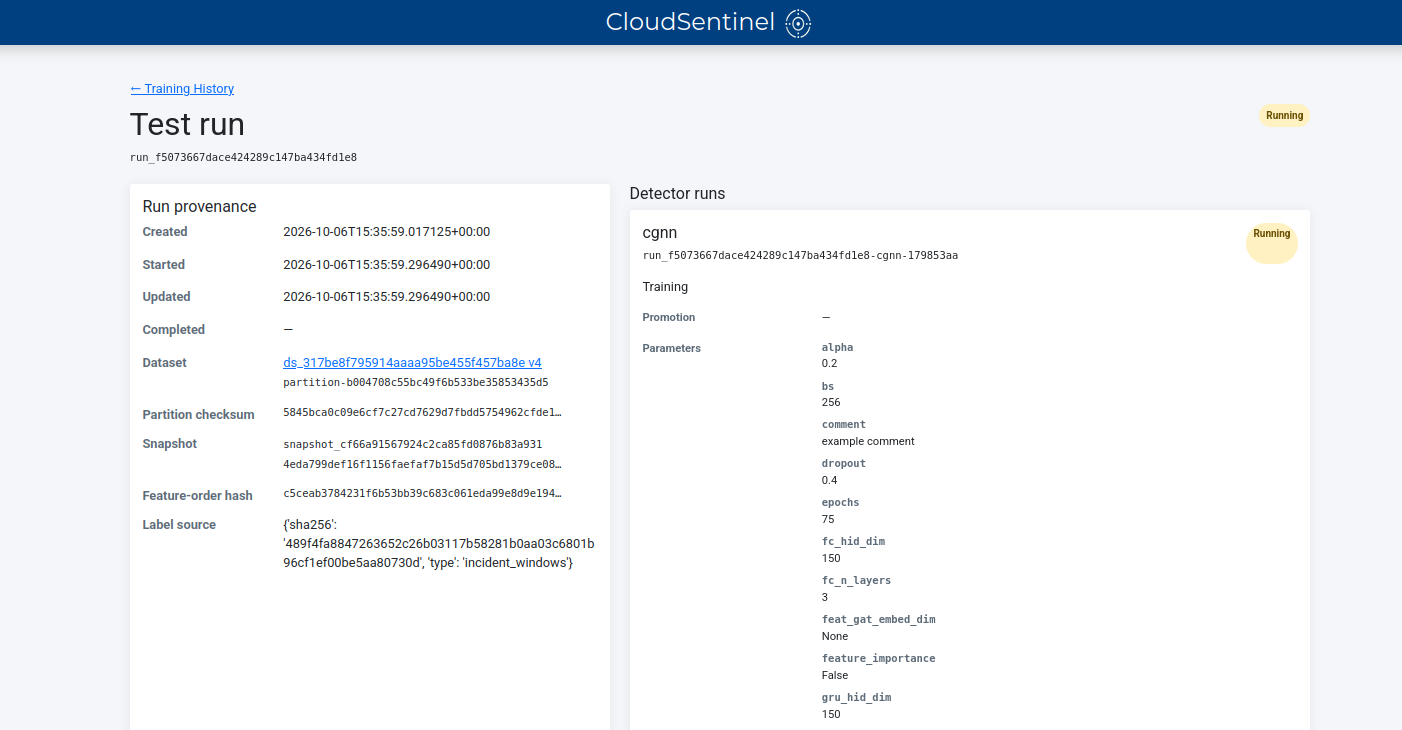
\includegraphics[width=1\linewidth]{figures/implementation/Models_and_training/training_workflow/Screenshot from 2026-10-06 17-37-54.png}
    \caption{Training run detail showing shared provenance and the independent lifecycle of each detector child.}
    \label{fig:training_run_detail}
\end{figure}

\subsubsection{Saved Models and inference readiness}

A successful Saved Model record retains the detector identifier and version, exact plugin reference, training run and child identifiers, dataset version and partition, immutable snapshot hash, feature identity, validated parameters, compact evaluation, promotion result, model metadata, and creation time. Repeated delivery of the same successful lifecycle event reuses the first record instead of creating a second model with different timestamps.

Inference-enabled training results additionally store the logical artefact identifier, the checksum of its manifest, the declared artefact format, and an inference status. A status of \texttt{ready} means that the generic runtime has the evidence needed to verify and load the immutable artefact. Older records without this evidence remain readable but are not silently treated as inference-ready. At activation time, the runtime checks the Saved Model, all artefact hashes, feature identity, and pinned adapter before loading the model.

The training section stops at this publication boundary. Sending live or uploaded metric matrices to an activated model belongs to the anomaly-detection runtime rather than to model training. This distinction keeps the explanation focused while showing why preprocessing objects, feature order, and plugin references must already be preserved during training.

\subsubsection{In-application detector onboarding}

The Add detector page closes the gap between the documented plugin contract and the usable training workflow. As shown in Figure~\ref{fig:detector_onboarding}, the operator can build the manifest through a form or upload an existing \texttt{manifest.yaml}. The same submission includes \texttt{adapter.py}, a pinned \texttt{requirements.lock}, and optional supporting Python files. Manifest parameters become fields in the generic training form, so the page is not limited to one fixed detector configuration.

Validation and publication are separate actions. Validation checks the package layout, manifest schema, dependency compatibility, entry point, and declared training and inference methods. Publication stores an immutable detector release; activation remains an explicit choice. Both publication actions require an operator access key. The key protects the action rather than sandboxing the supplied Python: uploaded detector code is still trusted server-side code and should only be accepted from an authorised developer or operator.

The page also keeps the contract understandable. It lists the required \texttt{validate\_training} and \texttt{run\_training} methods and the optional \texttt{load\_model} and \texttt{predict\_inference} methods used for live monitoring. Longer examples, the starter package, role separation, and a pre-publication checklist remain below the form. Invalid manifests, duplicate identifiers, unavailable repositories, and similar problems are translated into bounded explanations; raw paths and exception details are not displayed.

\begin{figure}[H]
    \centering
    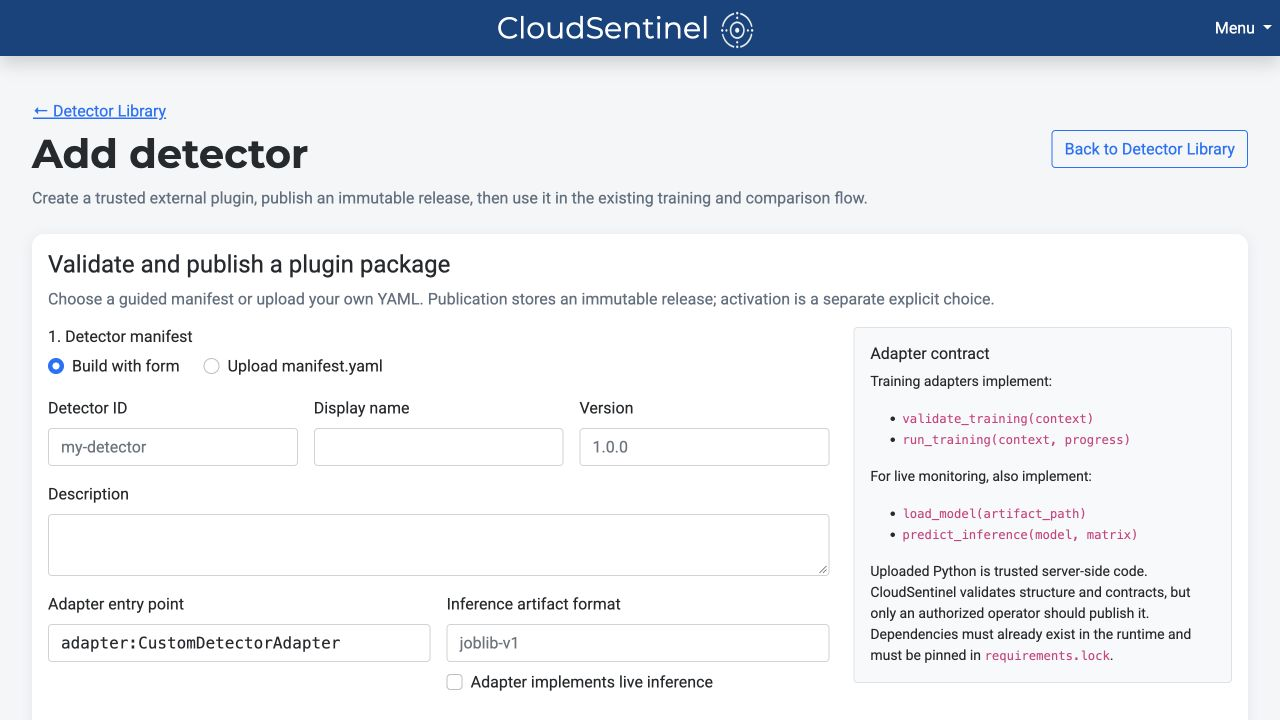
\includegraphics[width=1\linewidth]{figures/implementation/current/add_detector.jpg}
    \caption{Protected Add detector workflow with a form-based or uploaded manifest, implementation files, and the adapter contract.}
    \label{fig:detector_onboarding}
\end{figure}

Dependency declarations remain compatibility checks rather than installation requests: publication never installs packages into the running service. Changed code must be published under a new version because releases are immutable. This gives researchers a practical route for adding an algorithm while preserving the existing trust and reproducibility boundaries.

\subsubsection{Deployment and implementation boundaries}

The Learning API and Celery worker use shared persistent storage for dataset snapshots, training runs, model records, and published model artefacts. The Learning API receives controlled write access to the plugin repository so that the protected page can publish a validated release. Training workers and the generic detection runtime use the resulting activated releases. The containers run as a non-root user and public API projections remove repository paths and entry points.

These controls do not turn a detector plugin into untrusted sandboxed code. An activated plugin runs inside the worker process and is therefore accepted only from trusted developers or operators. Dependencies cannot be added dynamically, release signing is not yet implemented, and old releases are not automatically garbage-collected. The current runtime profiles also mean that a plugin requiring a new library still needs a planned runtime-image update.

The persistence layer is file-backed and intended for the controlled single-node staging environment used in this study. Its locks protect processes that share one filesystem, but a multi-node production deployment would require suitable shared storage or a database and stronger distributed coordination. Child tasks are logically independent, while physical parallelism still depends on separate Celery queues or sufficient workers. CGNN also retains process-global configuration in parts of its original implementation, so unrestricted concurrent CGNN training would require further isolation.

\subsubsection{Resulting workflow}

The resulting workflow connects detector extension and model training without detector-specific orchestration. A developer supplies a manifest, adapter, dependency lock, and optional implementation modules. A trusted operator validates and publishes an immutable release and explicitly activates it. The detector then appears in the existing library with its requirements and parameters. A user selects an exact catalogue partition and one or more compatible detectors, reviews their manifest-driven configuration, and starts one parent run.

CloudSentinel verifies the shared input, pins the plugin releases, and dispatches independent children. Each adapter applies its own preprocessing, trains and evaluates the detector, and returns a declared artefact. The generic executor validates and publishes that artefact, creates a safe Saved Model record, and retains the complete dataset, feature, parameter, and plugin provenance. Adding a compatible detector therefore no longer requires a new training page, detector-specific HTTP endpoint, or separate model-management implementation.

\subsection{Model Comparisons}

The Model Comparisons component connects the two preceding implementation areas. The Data Catalogue supplies a fixed evaluation partition, while the model catalogue supplies immutable trained model artefacts. The comparison workflow executes at least two compatible artefacts on the same observations and stores the resulting accuracy, timing, runtime, and provenance information as one persistent ComparisonRun. The aim is not to declare that one detector type is always better. It is to make a controlled comparison possible for one evaluation context and to retain enough information to understand the result later.

The implementation was introduced in two stages. The first stage added creation, execution, persistence, and inspection of individual comparisons. The second stage added historical robustness analysis, in which the same exact model artefact is examined across multiple stored workload contexts. Both stages concern anomaly detection only. Model training, root-cause analysis, remediation, export, and automatic model selection remain outside this component.

\subsubsection{Implementation overview}

Figure~\ref{fig:comparison_architecture} shows the components involved. The Django interface obtains evaluation datasets, compatible Saved Models, previous ComparisonRuns, and result views from the learning-adaptation API. When the user submits a comparison, the API validates and stores its complete definition before sending one asynchronous task to a Celery worker. The worker downloads a verified evaluation bundle from the Data Catalogue and asks the Generic Detection Runtime to evaluate each selected model. Compact results are written to comparison storage and later projected through safe public endpoints.

\begin{figure}[H]
    \centering
    \resizebox{0.98\linewidth}{!}{%
    \begin{tikzpicture}[
        font=\small,
        node distance=11mm and 12mm,
        component/.style={draw, rounded corners=2pt, align=center, minimum height=11mm, text width=28mm, fill=blue!7},
        external/.style={draw, rounded corners=2pt, align=center, minimum height=11mm, text width=28mm, fill=orange!11},
        storage/.style={draw, cylinder, shape border rotate=90, aspect=0.25, align=center, minimum height=14mm, text width=29mm, fill=green!10},
        flow/.style={-{Latex[length=2mm]}, thick},
        internal/.style={-{Latex[length=2mm]}, thick, dashed}
    ]
        \node[component] (ui) {Django comparison interface};
        \node[component, right=of ui] (api) {Learning-adaptation API};
        \node[component, right=of api] (worker) {Comparison Celery worker};
        \node[external, below=17mm of api, xshift=-21mm] (catalogue) {Data Catalogue evaluation bundle};
        \node[external, below=17mm of worker, xshift=21mm] (runtime) {Generic Detection Runtime};
        \node[storage, above=16mm of worker] (models) {Saved Model and artifact stores};
        \node[storage, below=21mm of worker, xshift=-19mm] (comparisons) {Immutable ComparisonRun files};

        \draw[flow] (ui) -- node[above, font=\scriptsize] {HTTP} (api);
        \draw[flow] (api) -- node[above, font=\scriptsize] {Redis task} (worker);
        \draw[flow] (catalogue) -- node[left, font=\scriptsize] {verified data} (worker);
        \draw[internal] (models) -- node[right, font=\scriptsize] {activate exact artefact} (runtime);
        \draw[flow] (worker) -- node[right, font=\scriptsize] {bounded evaluation} (runtime);
        \draw[flow] (api) -- (comparisons);
        \draw[flow] (worker) -- (comparisons);
    \end{tikzpicture}%
    }
    \caption{Implemented architecture for creating, executing, storing, and inspecting anomaly-detection comparisons.}
    \label{fig:comparison_architecture}
\end{figure}

The browser never calls the Data Catalogue transport endpoint or Generic Detection Runtime directly. Their addresses are server-side configuration and are not accepted from a comparison request. Public responses omit filesystem paths, service URLs, adapter entry points, task identifiers, model bytes, full prediction arrays, and stack traces.

\subsubsection{Comparison definition and scope}

A comparison evaluates concrete Saved Model artefacts rather than detector names in the abstract. Two CGNN records produced by different training runs are different comparison candidates, even when they use the same detector version. Conversely, one exact Saved Model can appear in several ComparisonRuns when it is evaluated against different workload contexts. This distinction is necessary because preprocessing, parameters, training data, and trained weights belong to the model artefact, not merely to the detector name.

Every ComparisonRun contains one shared evaluation dataset and at least two selected Saved Models. All models receive the same matrix, timestamps, labels, and incident context. This removes an important source of unfairness: if models were evaluated on different observations, a difference in F1 or runtime could not be attributed to the models alone. The component does not retrain or tune models and does not change their thresholds during comparison.

\subsubsection{Selecting an evaluation dataset}

The Data Catalogue exposes only available dataset versions with an explicit active partition as evaluation candidates. The comparison uses the test part of that partition. Its stored context contains the dataset identifier, display name, version, partition identifier and checksum, modality, observation count, evaluation start and end time, feature order and hash, workload context, label availability, and known incident windows.

Labels and timestamps are optional at the comparison transport level. An unlabelled partition can still be used to inspect model execution, anomaly scores, predicted anomaly positions, and runtime. Precision, recall, F1, the confusion matrix, and lead time are then marked unavailable rather than being assigned a fabricated value. Timestamps are required for a timeline with real dates and for detection timing relative to a known incident.

\subsubsection{Selecting compatible Saved Models}

Model compatibility is calculated by the learning-adaptation service. A candidate must be available, have inference status \texttt{ready}, use the supported \texttt{cloudsentinel.inference/v1} contract, and contain a logical artifact identifier and artifact-manifest checksum. Its modality and feature-order hash must exactly match the selected evaluation dataset. At least two compatible models are required.

Figure~\ref{fig:comparison_compatibility} summarises these checks. They do not branch on detector identifier. CGNN, Isolation Forest, Local Outlier Factor, or a later external detector can therefore participate through the same route when its saved artefact implements the shared inference contract. Incompatible records remain visible in the selection interface with safe reasons, but cannot be selected.

\begin{figure}[H]
    \centering
    \resizebox{0.94\linewidth}{!}{%
    \begin{tikzpicture}[
        font=\small,
        node distance=11mm and 15mm,
        dataset/.style={draw, rounded corners=2pt, align=left, minimum height=24mm, text width=42mm, fill=orange!11},
        check/.style={draw, rounded corners=2pt, align=left, minimum height=24mm, text width=48mm, fill=blue!7},
        model/.style={draw, rounded corners=2pt, align=center, minimum height=11mm, text width=36mm, fill=green!10},
        rejected/.style={draw, rounded corners=2pt, align=center, minimum height=11mm, text width=36mm, fill=red!8},
        flow/.style={-{Latex[length=2mm]}, thick}
    ]
        \node[dataset] (data) {\textbf{Evaluation partition}\\modality\\feature-order hash\\partition checksum};
        \node[check, right=of data] (checks) {\textbf{Compatibility checks}\\available and inference-ready\\supported contract\\same modality and feature identity\\complete artifact metadata};
        \node[model, right=of checks, yshift=17mm] (a) {Compatible Saved Model A};
        \node[model, right=of checks] (b) {Compatible Saved Model B};
        \node[rejected, right=of checks, yshift=-17mm] (c) {Incompatible model with reasons};

        \draw[flow] (data) -- (checks);
        \draw[flow] (checks) -- (a);
        \draw[flow] (checks) -- (b);
        \draw[flow] (checks) -- (c);
    \end{tikzpicture}%
    }
    \caption{Model selection is based on inference readiness and exact input compatibility rather than detector-specific routes.}
    \label{fig:comparison_compatibility}
\end{figure}

\subsubsection{Pinning comparison provenance}

The API re-reads the dataset and model records when the final request is submitted. It then stores snapshots of the dataset identity, feature identity, workload context, selected model metadata, and exact artifact identity. The artifact identity contains the model identifier, logical artifact identifier, artifact-manifest checksum, inference contract, and artifact format. The comparison also records its own identifier, name, schema and configuration version, creation time, and a client-generated request identifier.

This information is captured before task dispatch. A model activation or catalogue update that occurs afterwards cannot silently change what the queued comparison intends to evaluate. The worker later verifies that the evaluation bundle still has the recorded feature hash and that the runtime evaluated the recorded artifact-manifest hash. A mismatch is treated as an integrity failure.

The client request identifier makes final submission idempotent. Repeating the same browser submission reuses the already stored ComparisonRun instead of creating two tasks. The wizard also disables repeated submission in the browser, but server-side idempotency remains the authoritative protection.

\subsubsection{Evaluation bundle and integrity checks}

The worker requests a streamed \texttt{metrics-evaluation/v1} ZIP archive from the Data Catalogue. Figure~\ref{fig:comparison_evaluation_bundle} shows its allowed contents. The manifest and matrix are required. Labels and timestamps are present only when the catalogue version provides them. No other files or nested paths are accepted.

\begin{figure}[H]
    \centering
    \resizebox{0.91\linewidth}{!}{%
    \begin{tikzpicture}[
        font=\small,
        node distance=10mm and 12mm,
        root/.style={draw, rounded corners=2pt, align=center, minimum height=10mm, text width=35mm, fill=blue!9},
        required/.style={draw, rounded corners=2pt, align=left, minimum height=14mm, text width=38mm, fill=green!10},
        optional/.style={draw, rounded corners=2pt, align=left, minimum height=14mm, text width=38mm, fill=gray!10},
        flow/.style={-{Latex[length=2mm]}, thick}
    ]
        \node[root] (bundle) {\texttt{metrics-evaluation/v1}};
        \node[required, below left=of bundle, xshift=-22mm] (manifest) {\textbf{\texttt{manifest.json}}\\dataset and partition identity, feature order, file hashes, counts, context};
        \node[required, below=of bundle] (matrix) {\textbf{\texttt{matrix.csv}}\\headerless numeric evaluation observations};
        \node[optional, below right=of bundle, xshift=22mm] (labels) {\textbf{\texttt{labels.csv}}\\optional binary ground truth};
        \node[optional, below=26mm of bundle] (timestamps) {\textbf{\texttt{timestamps.csv}}\\optional UTC observation times};

        \draw[flow] (bundle) -- (manifest);
        \draw[flow] (bundle) -- (matrix);
        \draw[flow] (bundle) -- (labels);
        \draw[flow] (bundle) -- (timestamps);
    \end{tikzpicture}%
    }
    \caption{Allowed files in the verified evaluation bundle. Labels and timestamps are optional.}
    \label{fig:comparison_evaluation_bundle}
\end{figure}

Verification checks the archive size, safe filenames, declared file checksums, dataset and partition identity, feature order and hash, observation and feature counts, rectangular numeric matrix shape, binary label values, and timestamp coverage. The worker extracts the bundle into a temporary private directory and removes it after the task. It does not create a second persistent copy of the evaluation matrix. A damaged archive, unsafe filename, changed feature identity, or inconsistent row count stops execution before a model result is accepted.

\subsubsection{Generic comparison execution pipeline}

Figure~\ref{fig:comparison_execution_pipeline} shows the execution sequence. The ComparisonRun is first changed from \texttt{queued} to \texttt{running}. After bundle verification, the worker processes the selected models one by one inside the same Celery task. Before each call it marks the corresponding result as running. It then activates the exact Saved Model in the Generic Detection Runtime and sends the matrix with its authoritative feature identity to the internal evaluation endpoint.

\begin{figure}[H]
    \centering
    \resizebox{0.98\linewidth}{!}{%
    \begin{tikzpicture}[
        font=\small,
        node distance=8mm,
        phase/.style={draw, rounded corners=2pt, align=center, minimum height=11mm, text width=27mm, fill=blue!7},
        model/.style={draw, rounded corners=2pt, align=center, minimum height=11mm, text width=29mm, fill=orange!10},
        output/.style={draw, rounded corners=2pt, align=center, minimum height=11mm, text width=28mm, fill=green!10},
        flow/.style={-{Latex[length=2mm]}, thick}
    ]
        \node[phase] (persist) {Persist pinned ComparisonRun};
        \node[phase, right=of persist] (bundle) {Download and verify bundle};
        \node[phase, right=of bundle] (running) {Set comparison to running};
        \node[model, below=15mm of running, xshift=-32mm] (activate) {Activate exact model artefact};
        \node[model, below=15mm of running] (evaluate) {Evaluate matrix in generic runtime};
        \node[model, below=15mm of running, xshift=32mm] (verify) {Verify output and artifact hash};
        \node[output, below=16mm of evaluate, xshift=-22mm] (metrics) {Calculate metrics, timing, and bounded timeline};
        \node[output, below=16mm of evaluate, xshift=22mm] (finish) {Persist model result and terminal status};

        \draw[flow] (persist) -- (bundle);
        \draw[flow] (bundle) -- (running);
        \draw[flow] (running) -- (activate);
        \draw[flow] (activate) -- (evaluate);
        \draw[flow] (evaluate) -- (verify);
        \draw[flow] (verify) -- (metrics);
        \draw[flow] (metrics) -- (finish);
    \end{tikzpicture}%
    }
    \caption{Execution pipeline for one ComparisonRun. Each model follows the activation, evaluation, verification, and persistence steps.}
    \label{fig:comparison_execution_pipeline}
\end{figure}

The runtime returns binary predictions, anomaly scores, warm-up observations, runtime, detector identity, model identity, and artifact-manifest hash. The worker validates types, lengths, finite values, binary semantics, non-negative runtime, and the relation between warm-up and expected observations. It then calculates comparison metrics and stores only a bounded public representation. A failure for one model is converted into a safe failed result and the worker continues with the remaining models.

This implementation provides independent result handling, but not distributed fan-out. One task evaluates the selected models sequentially. This is sufficient for the controlled staging environment and avoids multiple copies of the evaluation bundle, but a large production comparison service could instead dispatch bounded child tasks and coordinate their results.

\subsubsection{Accuracy metrics}

When labels are available, CloudSentinel interprets \texttt{0} as normal and \texttt{1} as anomalous. Table~\ref{tab:comparison_confusion_matrix} shows the four possible combinations between ground truth and prediction. These counts are stored together with precision, recall, and F1.

\begin{table}[H]
    \centering
    \caption{Confusion matrix used for labelled comparison results.}
    \label{tab:comparison_confusion_matrix}
    \begin{tabular}{@{}lcc@{}}
        \toprule
        & \textbf{Predicted normal} & \textbf{Predicted anomaly} \\
        \midrule
        \textbf{Actually normal} & True negative & False positive \\
        \textbf{Actually anomalous} & False negative & True positive \\
        \bottomrule
    \end{tabular}
\end{table}

Precision describes which fraction of predicted anomalies were actually anomalous. Recall describes which fraction of known anomalous observations were detected. F1 is the harmonic mean of precision and recall and is high only when both are high. Division by zero produces a score of zero rather than a runtime error. The detail page may identify one model with the highest F1, but only when labelled results exist and the highest value is unique. This is a deterministic summary of one context, not a claim that the model is best in general.

\subsubsection{Warm-up and detection lead time}

Sequence-based models can require earlier observations before producing their first valid prediction. The generic runtime reports this as a warm-up count. The worker removes the same leading observations from labels and timestamps before checking lengths or calculating metrics. Models without sequence windows report zero warm-up. This produces a fair alignment between every prediction and its corresponding ground-truth row.

Detection lead time uses the first predicted anomaly after warm-up and the start of the first known incident window. Figure~\ref{fig:comparison_lead_time} shows the implemented meaning. The calculation is incident start minus first detection time. A non-negative result means that the model detected an anomaly before or exactly at the incident start. When the first detection occurs later, the interface states that detection occurred after incident start rather than presenting a negative number as positive lead time.

\begin{figure}[H]
    \centering
    \resizebox{0.88\linewidth}{!}{%
    \begin{tikzpicture}[
        font=\small,
        marker/.style={draw, rounded corners=2pt, align=center, minimum height=10mm, text width=31mm},
        flow/.style={-{Latex[length=2mm]}, very thick}
    ]
        \draw[flow] (0,0) -- (12,0) node[right] {time};
        \fill[gray!18] (0,-0.65) rectangle (2.2,0.65);
        \node[font=\scriptsize] at (1.1,0) {warm-up};
        \draw[very thick, blue!70] (4,0.35) -- (4,-0.35);
        \node[marker, fill=blue!7] at (4,1.15) {first detected anomaly};
        \draw[very thick, red!75] (8,0.45) -- (8,-0.45);
        \node[marker, fill=red!8] at (8,1.15) {known incident start};
        \draw[<->, thick] (4,-0.8) -- node[below] {positive lead time} (8,-0.8);
        \fill[red!12] (8,-0.48) rectangle (10.8,0.48);
        \node[font=\scriptsize] at (9.4,0) {incident window};
    \end{tikzpicture}%
    }
    \caption{Lead time is the interval between the first valid anomaly detection and the known incident start.}
    \label{fig:comparison_lead_time}
\end{figure}

Missing timestamps, no detected anomaly, missing incident context, a detection after the incident start, and unavailable ground truth are represented by separate statuses. They are never converted into a zero-second lead time, because zero would incorrectly suggest a detection exactly at incident start.

\subsubsection{Bounded timeline representation}

For every successful model, the worker combines timestamps, predictions, and anomaly scores into timeline points. Full arrays remain between the worker and internal runtime for the duration of the task. The stored timeline is sampled to a configured maximum number of points, while detected anomaly positions are retained within that bounded representation. This keeps ComparisonRun files and browser responses manageable for long evaluation periods.

The visual timeline overlays model score series and shades known incident windows. Larger points identify predicted anomalies. Scores from different detector types can use different numerical scales; an Isolation Forest score and a CGNN reconstruction score do not have the same unit. The chart is therefore intended for temporal inspection: it shows when scores changed and when anomalies were produced, but the absolute height of one detector's line should not be interpreted as directly better than another's.

\subsubsection{Comparison lifecycle and persistence}

ComparisonRuns are stored as JSON records below a configured storage root. Creation and updates use atomic file replacement, and each record has a process-level lock. The normal lifecycle is shown in Figure~\ref{fig:comparison_lifecycle}. A newly accepted record is \texttt{queued}; the worker changes it to \texttt{running}; and the final state is \texttt{completed}, \texttt{partial}, or \texttt{failed}. Terminal records are immutable.

\begin{figure}[H]
    \centering
    \resizebox{0.88\linewidth}{!}{%
    \begin{tikzpicture}[
        font=\small,
        node distance=11mm,
        state/.style={draw, rounded corners=2pt, align=center, minimum height=11mm, text width=25mm, fill=blue!7},
        success/.style={draw, rounded corners=2pt, align=center, minimum height=11mm, text width=25mm, fill=green!11},
        partial/.style={draw, rounded corners=2pt, align=center, minimum height=11mm, text width=25mm, fill=orange!12},
        failure/.style={draw, rounded corners=2pt, align=center, minimum height=11mm, text width=25mm, fill=red!8},
        flow/.style={-{Latex[length=2mm]}, thick}
    ]
        \node[state] (queued) {\texttt{queued}};
        \node[state, right=of queued] (running) {\texttt{running}};
        \node[success, right=18mm of running, yshift=14mm] (completed) {\texttt{completed}\\all models succeed};
        \node[partial, right=18mm of running] (partial) {\texttt{partial}\\mixed results};
        \node[failure, right=18mm of running, yshift=-14mm] (failed) {\texttt{failed}\\no model succeeds};

        \draw[flow] (queued) -- (running);
        \draw[flow] (running) -- (completed);
        \draw[flow] (running) -- (partial);
        \draw[flow] (running) -- (failed);
    \end{tikzpicture}%
    }
    \caption{Durable lifecycle of a ComparisonRun. A model failure can produce a partial result without discarding successful siblings.}
    \label{fig:comparison_lifecycle}
\end{figure}

A run is completed only when all selected models succeed. It is partial when at least one succeeds and at least one fails, and failed when none succeeds or a comparison-wide error prevents meaningful execution. Each model result retains its own status and safe failure summary. Polling is performed through a Django proxy only while the run is queued or running. Requests do not overlap, and polling stops when a terminal state is reached or the user leaves the page.

\subsubsection{Comparison creation interface}

The comparison interface starts with the Past Comparisons page shown in Figure~\ref{fig:comparison_overview}. It provides search and filters for modality, workload, and lifecycle state. Each result shows its evaluation dataset and version, workload context, number of models, status, creation time, and a unique F1 winner when one exists. This makes completed comparisons persistent evaluation artefacts rather than temporary result pages.

\begin{figure}[H]
    \centering
    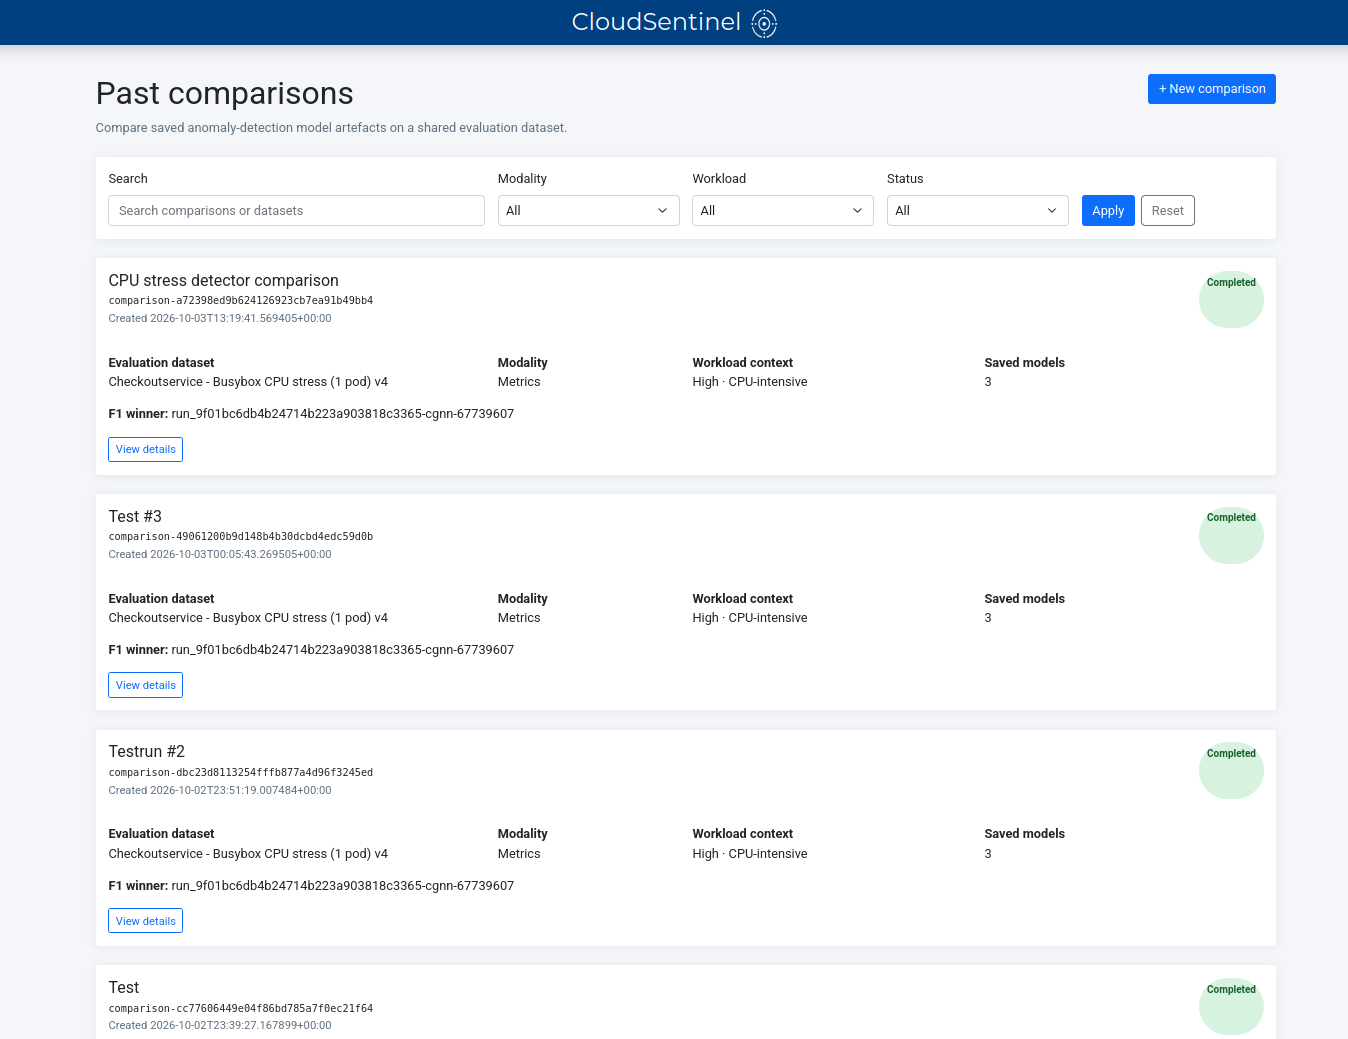
\includegraphics[width=1\linewidth]{figures/implementation/comparison/Screenshot from 2026-10-06 17-39-52.png}
    \caption{Past Comparisons overview with search, context filters, lifecycle status, dataset provenance, and result summary.}
    \label{fig:comparison_overview}
\end{figure}

The creation wizard contains three steps. In Figure~\ref{fig:comparison_select_dataset}, the user selects one shared evaluation partition. The card displays its modality, observation count, workload context, anomaly scenario, incident window, and ground-truth availability. Datasets without labels remain selectable, but the interface warns that accuracy and lead-time metrics may be unavailable.

\begin{figure}[H]
    \centering
    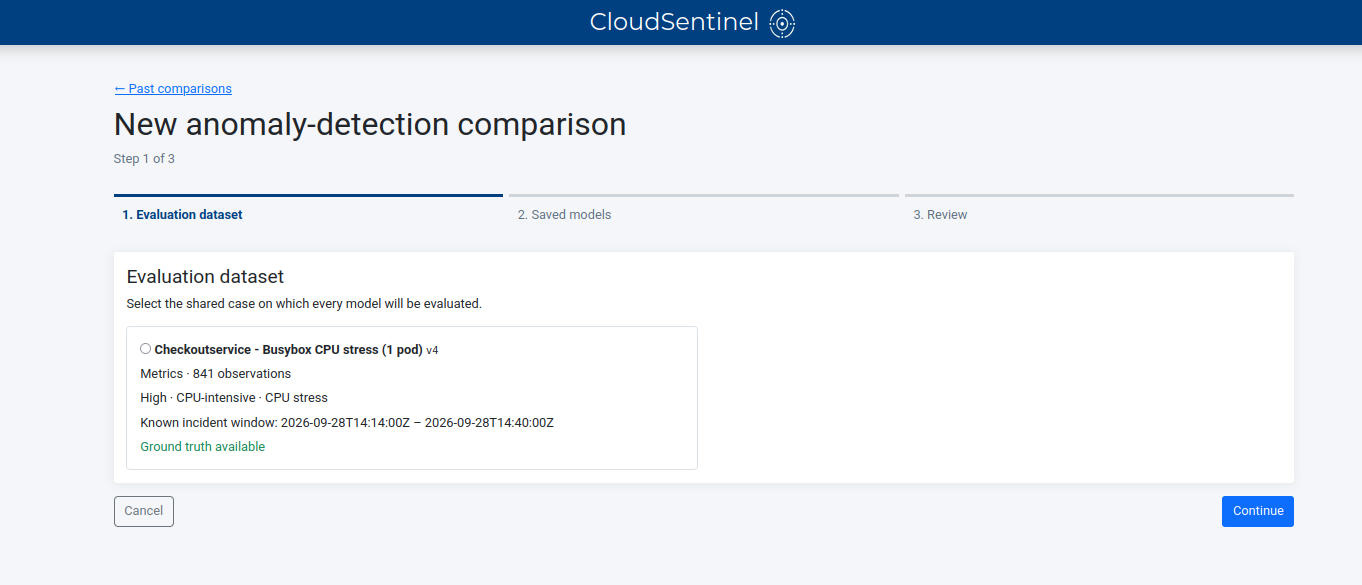
\includegraphics[width=1\linewidth]{figures/implementation/comparison/Screenshot from 2026-10-06 17-40-22.png}
    \caption{Step 1 of comparison creation: selecting the shared evaluation dataset and exact version.}
    \label{fig:comparison_select_dataset}
\end{figure}

Figure~\ref{fig:comparison_select_models} shows model selection. Compatible inference-ready artefacts can be selected, while incompatible records are disabled and accompanied by one or more reasons. The user must choose at least two. Displaying trained-on information and detector versions helps distinguish several Saved Models created with the same detector implementation.

\begin{figure}[H]
    \centering
    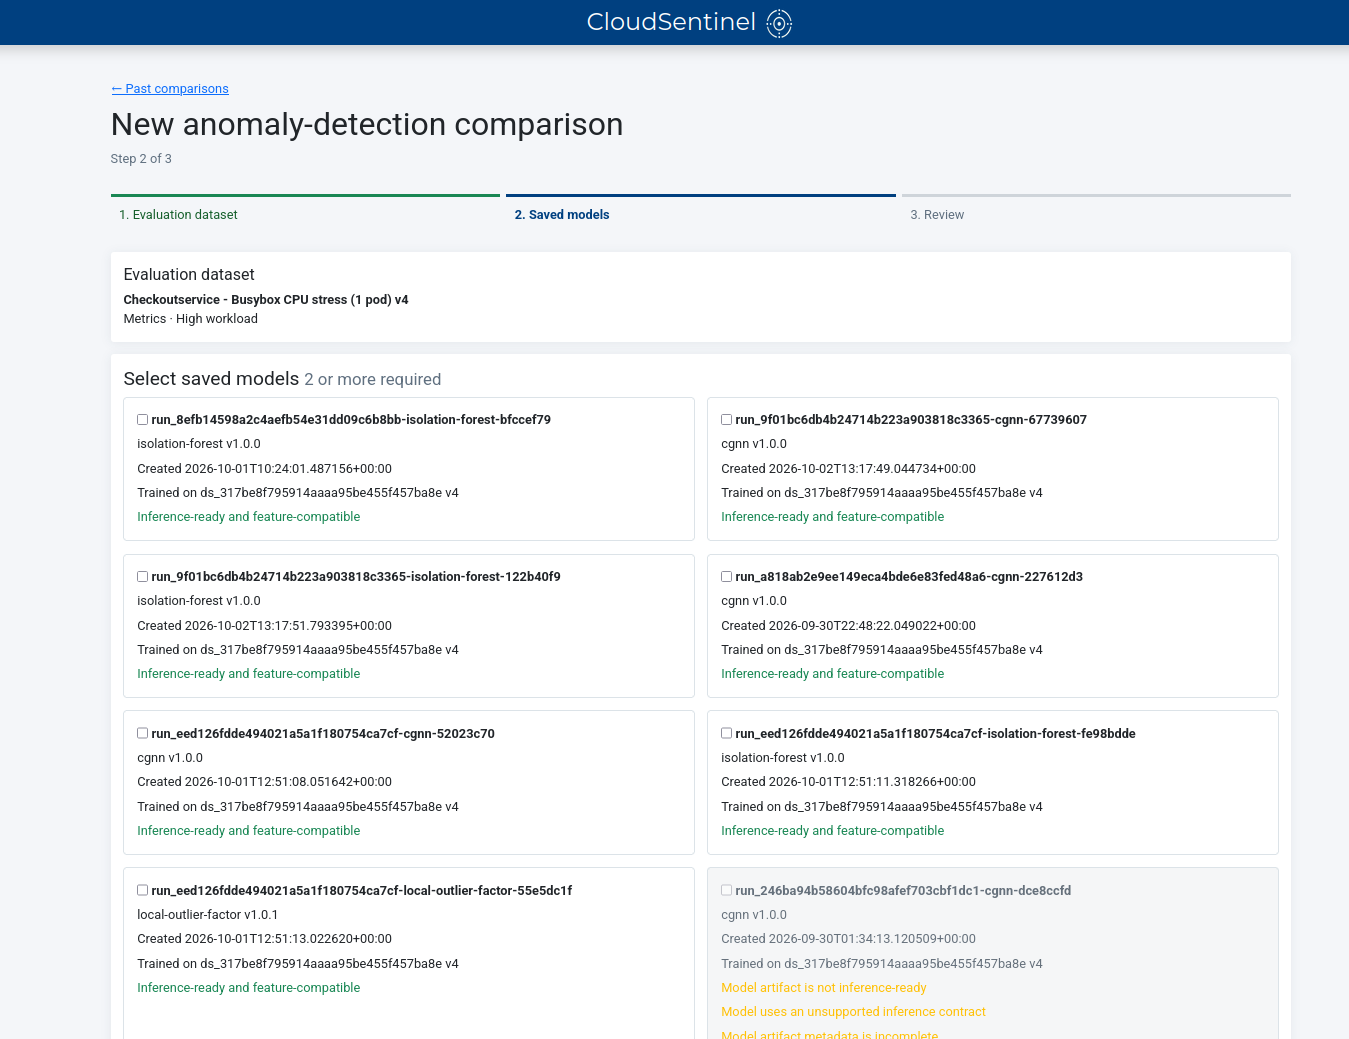
\includegraphics[width=1\linewidth]{figures/implementation/comparison/Screenshot from 2026-10-06 17-40-34.png}
    \caption{Step 2: selecting at least two inference-ready Saved Models with the same modality and feature identity.}
    \label{fig:comparison_select_models}
\end{figure}

The review page in Figure~\ref{fig:comparison_review} shows the comparison name, evaluation case, workload context, known incident window, selected artefacts, and planned measures. The wizard state is signed by Django between steps, so a user cannot safely alter stored selections through hidden form fields. Submission still triggers complete server-side validation because the signed browser state is not used as a substitute for current backend records.

\begin{figure}[H]
    \centering
    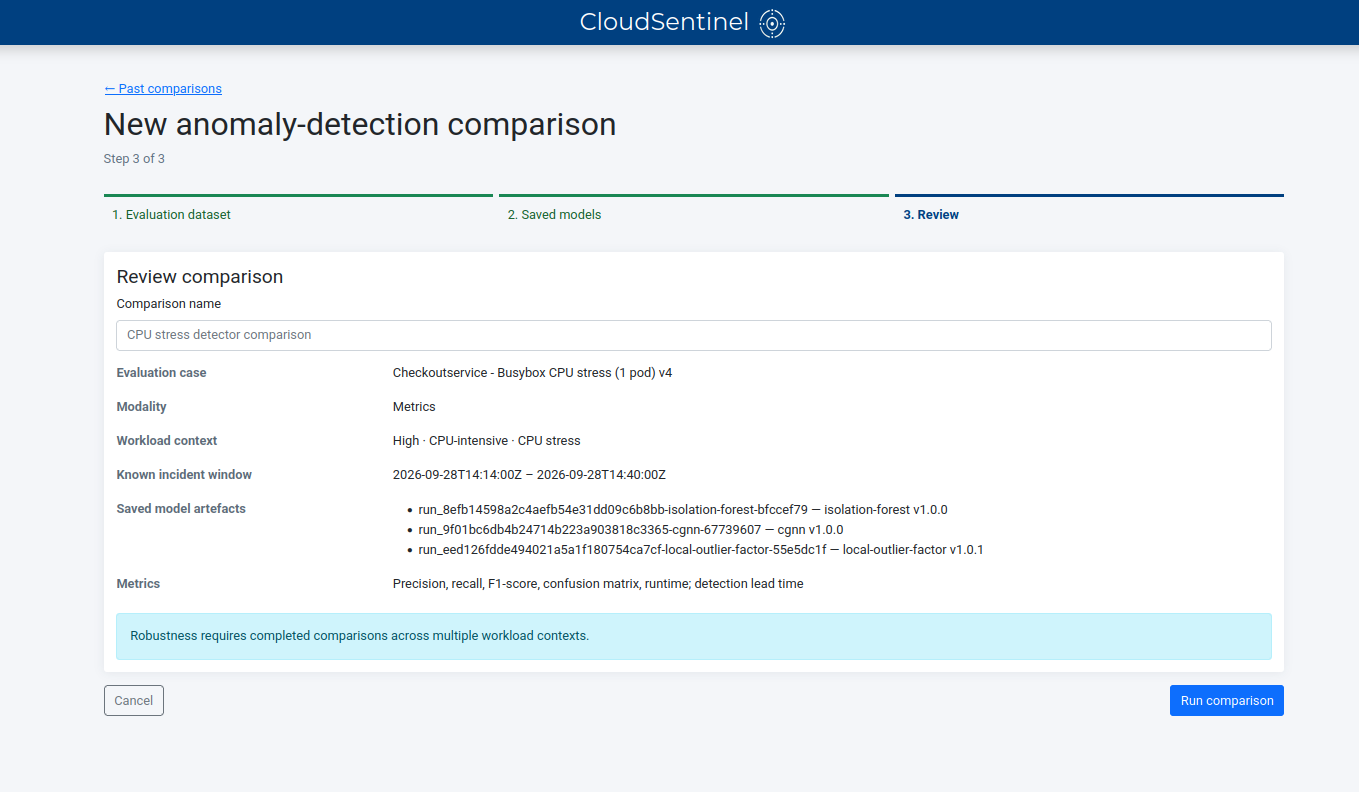
\includegraphics[width=1\linewidth]{figures/implementation/comparison/Screenshot from 2026-10-06 17-40-52.png}
    \caption{Step 3: reviewing dataset context, selected immutable artefacts, and available measures before dispatch.}
    \label{fig:comparison_review}
\end{figure}

\subsubsection{Comparison result overview}

The detail page keeps five result views under one ComparisonRun: Overview, Timeline, Model details, Experiment evidence, and Robustness. Figure~\ref{fig:comparison_result_overview} shows the Overview tab. It places precision, recall, F1, detection lead time, runtime, and per-model status in one table. Unavailable values remain explicit, and a partial comparison can show successful rows alongside safely reported failures.

\begin{figure}[H]
    \centering
    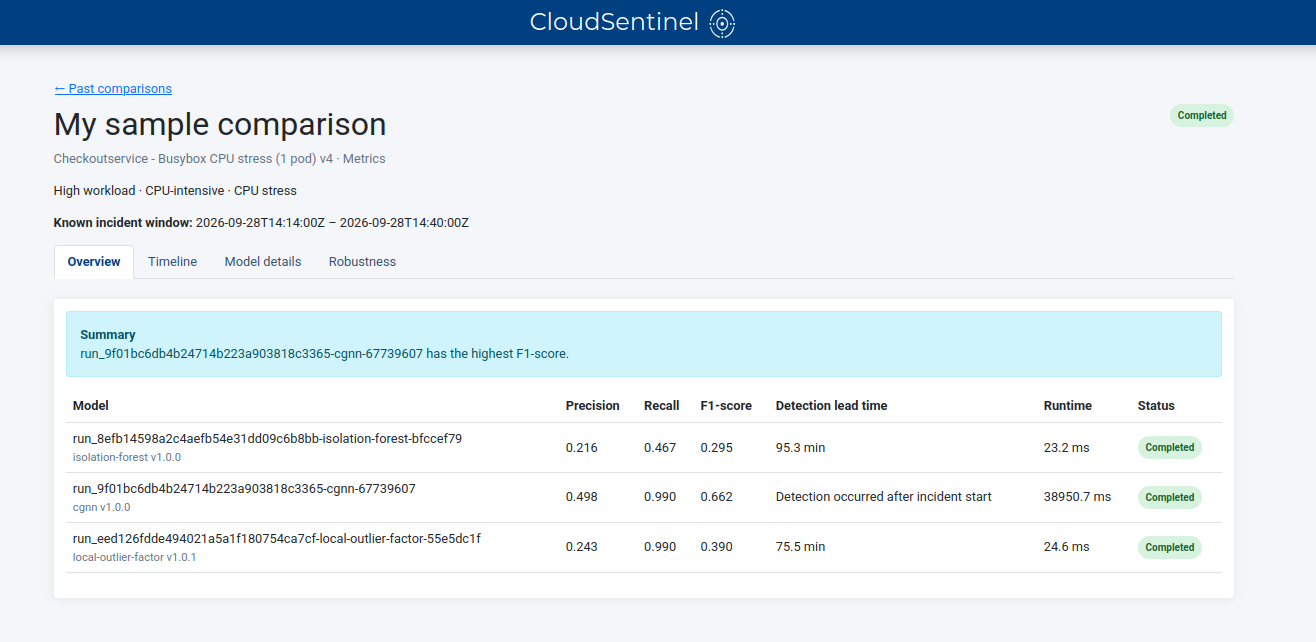
\includegraphics[width=1\linewidth]{figures/implementation/comparison/Screenshot from 2026-10-06 17-46-45.png}
    \caption{Comparison Overview with labelled accuracy, lead time, runtime, status, and the unique highest-F1 summary.}
    \label{fig:comparison_result_overview}
\end{figure}

The highest-F1 summary is deliberately narrow. It describes only this dataset partition and appears only when one successful labelled model has a strictly highest value. It does not combine runtime, lead time, robustness, operational cost, or explainability, and it does not promote or activate the model automatically.

\subsubsection{Timeline and model details}

Figure~\ref{fig:comparison_timeline} shows the Timeline tab. The known incident interval is displayed both as text and as a shaded area. Each model has its own score line, and detected anomaly positions are emphasised. This supports inspection of whether a model fired before, during, or after the known incident rather than relying only on aggregate counts.

\begin{figure}[H]
    \centering
    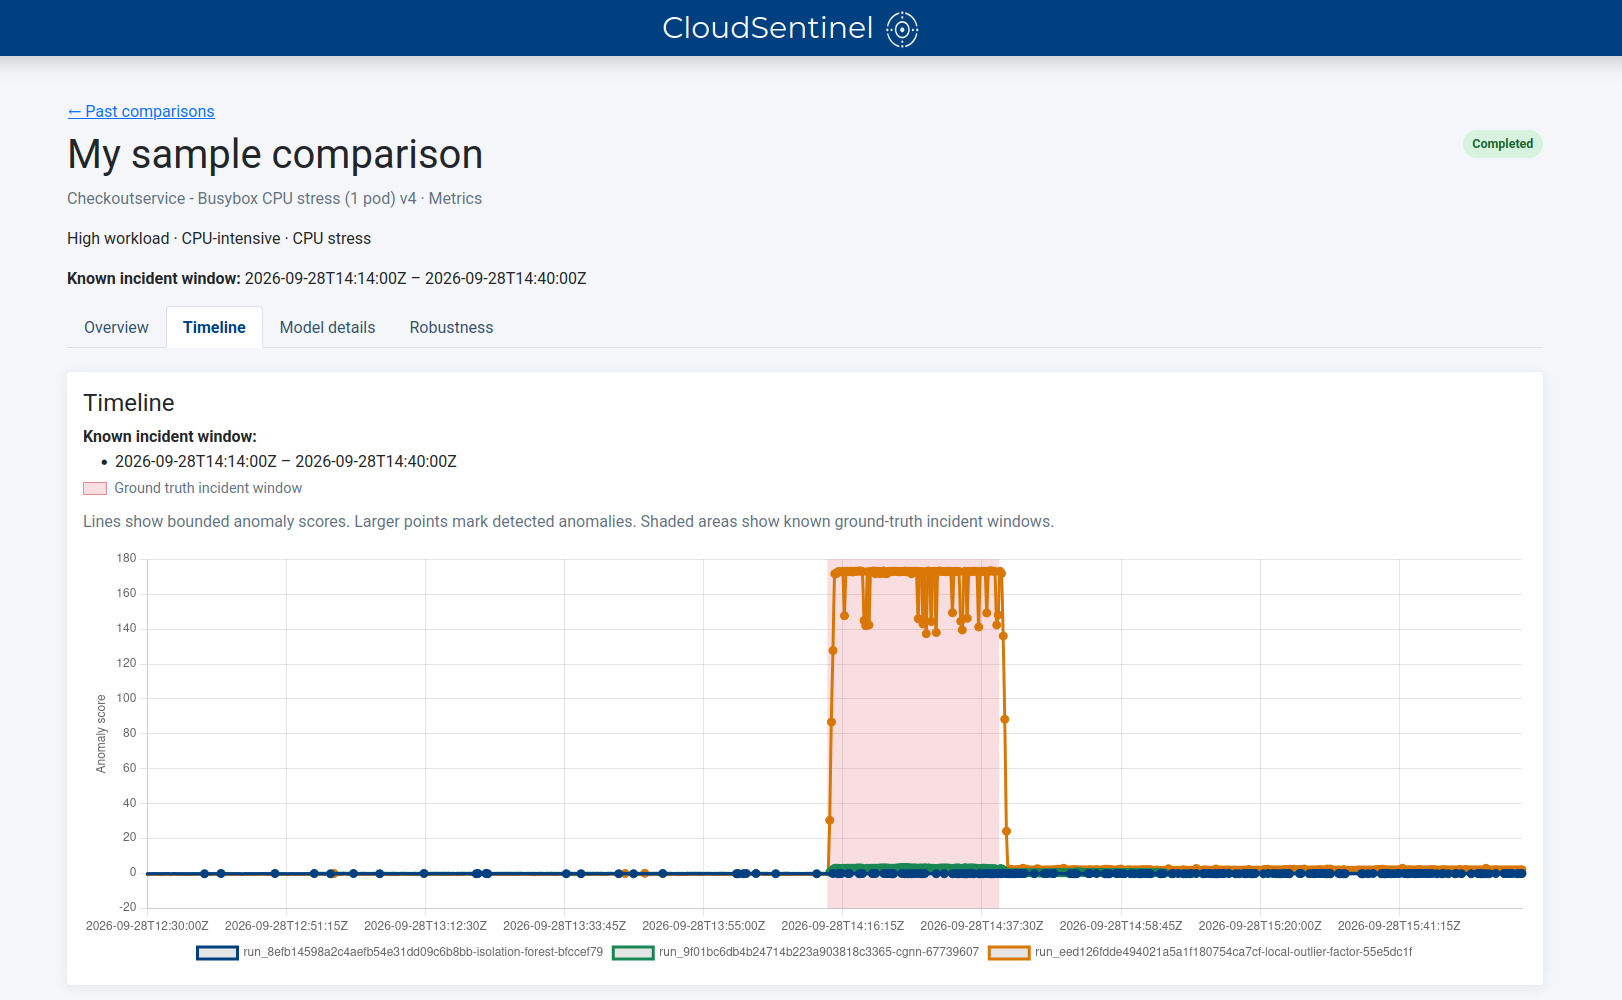
\includegraphics[width=1\linewidth]{figures/implementation/comparison/Screenshot from 2026-10-06 17-47-15.png}
    \caption{Bounded comparison timeline with anomaly scores, detected anomaly points, and the known ground-truth incident window.}
    \label{fig:comparison_timeline}
\end{figure}

The Model details tab in Figure~\ref{fig:comparison_model_details} retains the connection to the model-management pipeline. For every selected artefact it shows detector version, creation time, training source, exact artifact identity, evaluation outcome, runtime, and F1 when available. A direct link opens the full Saved Model provenance page. The comparison therefore does not duplicate all training metadata, but preserves and exposes the identity needed to retrieve it.

\begin{figure}[H]
    \centering
    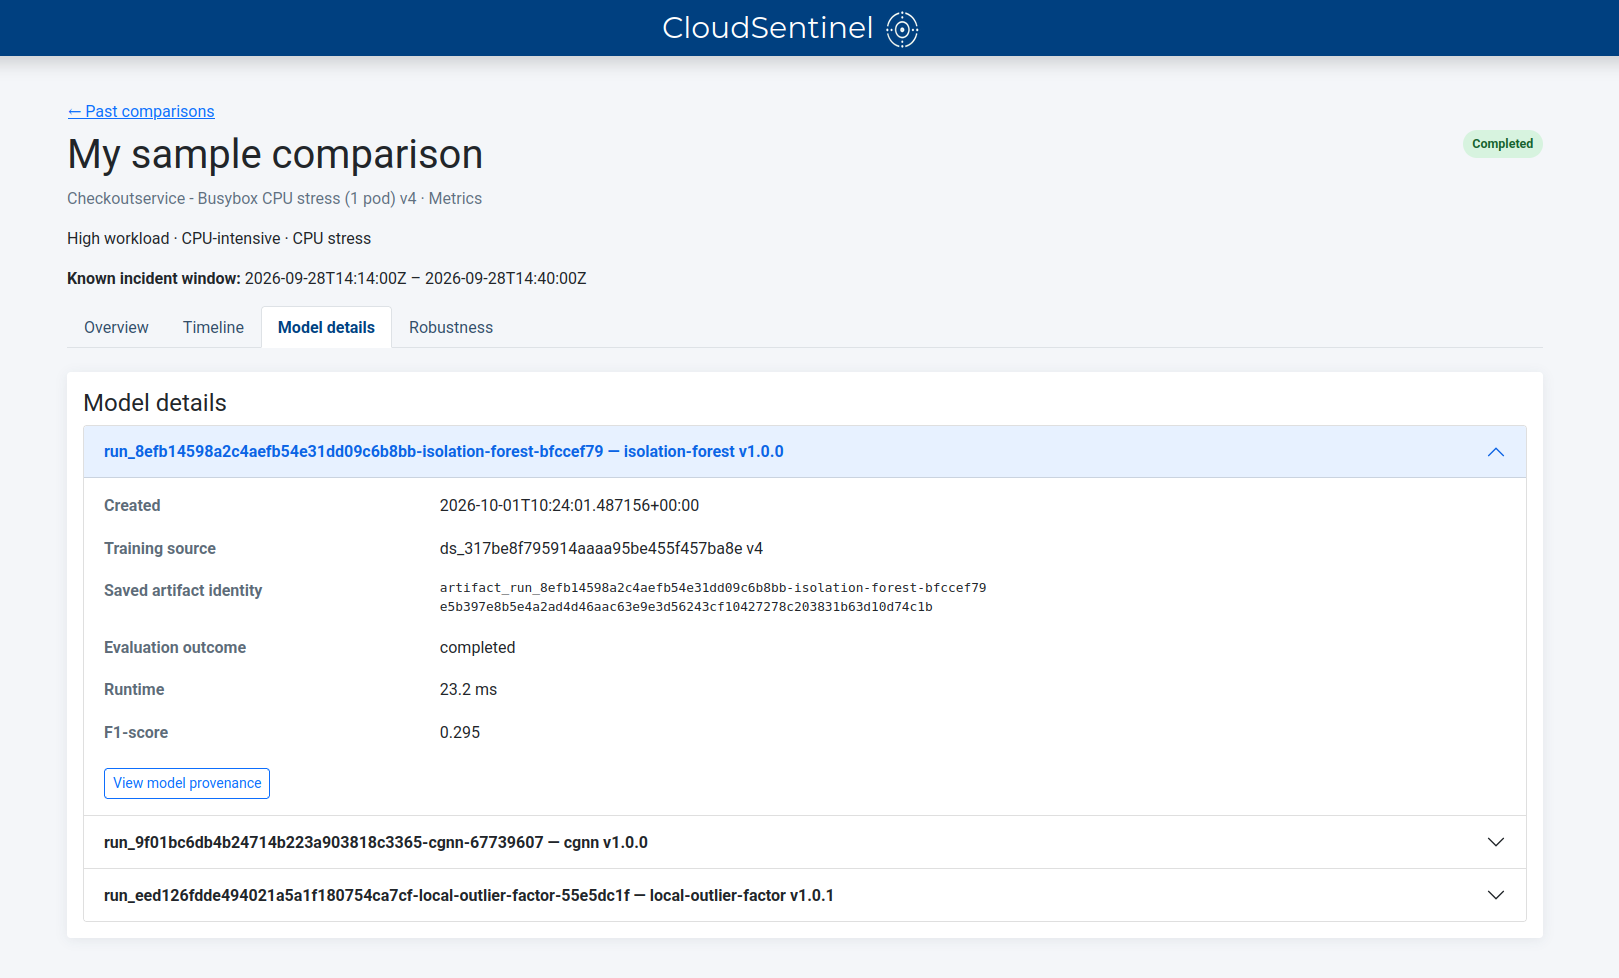
\includegraphics[width=1\linewidth]{figures/implementation/comparison/Screenshot from 2026-10-06 17-47-36.png}
    \caption{Model details for the exact artefacts used in the comparison, including links to their training provenance.}
    \label{fig:comparison_model_details}
\end{figure}

\subsubsection{Experiment evidence}

The Experiment evidence tab, shown in Figure~\ref{fig:comparison_experiment_evidence}, answers a different question from the score overview: what exactly produced these numbers? It records the evaluation dataset and partition, their checksums, feature-order hash, observation count, time window, label availability, workload context, and incident windows. It then lists the exact Saved Model artefacts, detector releases, training datasets, training runs, and evaluation status. All compared models share the same evaluation partition and feature order, while differences in their training source remain visible.

This view also states the limit of the result. It supports a direct comparison of these artefacts in this recorded context, but not a universal claim that one detector is best. Stability across contexts requires repeated comparisons of the same artefacts and is handled in the Robustness tab.

\begin{figure}[H]
    \centering
    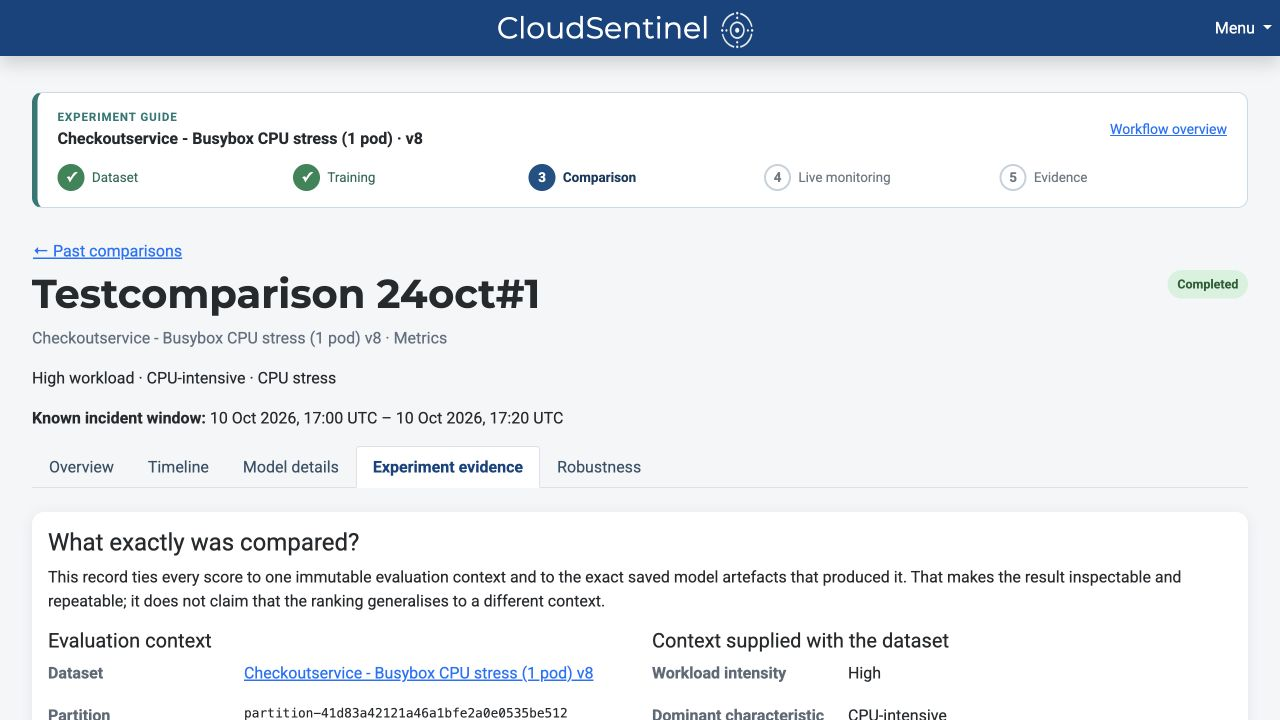
\includegraphics[width=1\linewidth]{figures/implementation/current/comparison_evidence.jpg}
    \caption{Experiment evidence tying comparison scores to the exact dataset partition, workload context, and immutable model artefacts.}
    \label{fig:comparison_experiment_evidence}
\end{figure}

\subsubsection{Historical robustness across workload contexts}

One ComparisonRun describes performance in one evaluation context. It cannot by itself show whether performance remains stable when workload intensity, workload characteristic, anomaly scenario, or evaluation data changes. The robustness extension therefore scans earlier immutable ComparisonRuns for repeated evaluations of the same exact Saved Model artefact.

The identity of a robustness series is the combination of model identifier, artifact identifier, and artifact-manifest checksum. Matching only the detector name, detector version, or training run would be too weak: separately trained artefacts can behave differently. Only completed and partial ComparisonRuns are eligible, and within them only completed model results contribute. Failed runs and failed children remain visible in their original comparison but cannot change robustness statistics.

Figure~\ref{fig:comparison_robustness_model} illustrates the aggregation. Independent partitions contribute separate workload contexts to one exact artefact. Unlabelled contexts contribute runtime and coverage, but not invented accuracy or lead-time values. At least two distinct contexts are required before the interface describes the evidence as sufficient for robustness assessment.

\begin{figure}[H]
    \centering
    \resizebox{0.93\linewidth}{!}{%
    \begin{tikzpicture}[
        font=\small,
        node distance=10mm and 17mm,
        context/.style={draw, rounded corners=2pt, align=center, minimum height=12mm, text width=36mm, fill=orange!11},
        artifact/.style={draw, rounded corners=2pt, align=center, minimum height=18mm, text width=43mm, fill=blue!8},
        aggregate/.style={draw, rounded corners=2pt, align=left, minimum height=22mm, text width=47mm, fill=green!10},
        flow/.style={-{Latex[length=2mm]}, thick}
    ]
        \node[context] (low) {Low workload\\partition A};
        \node[context, below=of low] (high) {High workload\\partition B};
        \node[context, below=of high] (network) {Network delay\\partition C};
        \node[artifact, right=of high] (model) {Exact Saved Model artefact\\model ID + artifact ID + manifest hash};
        \node[aggregate, right=of model] (stats) {\textbf{Historical robustness}\\context and labelled coverage\\median and F1 range\\runtime and lead-time coverage};

        \draw[flow] (low) -- (model);
        \draw[flow] (high) -- (model);
        \draw[flow] (network) -- (model);
        \draw[flow] (model) -- (stats);
    \end{tikzpicture}%
    }
    \caption{Robustness is derived from the same immutable model artefact evaluated in several independent contexts.}
    \label{fig:comparison_robustness_model}
\end{figure}

\subsubsection{Robustness statistics and fair context matching}

For each exact artefact, the API reports the number of distinct contexts and labelled contexts; median precision, recall, and F1; minimum and maximum F1; F1 range; population standard deviation when at least two F1 values exist; median, minimum, and maximum runtime; and available lead-time count with its median and range. Medians reduce the influence of one unusually high or low result, while range and standard deviation describe variation. The implementation intentionally does not combine these measures into one composite robustness score, because such a score would require an explicit and potentially subjective weighting.

Direct side-by-side rows are produced only for contexts shared by at least two artefacts currently shown. This shared-context matrix prevents a model evaluated only on an easy partition from being placed beside a model evaluated only on a difficult partition as though the values were directly comparable. Coverage differences produce an explicit warning, and the interface does not declare a robustness winner.

Repeated evaluation of the same exact artefact on the same partition checksum is deduplicated. The newest terminal ComparisonRun becomes canonical for that artefact-context pair. This prevents accidental retries from increasing the apparent number of independent contexts. Records that lack a strong partition checksum cannot participate because they cannot be deduplicated safely.

\subsubsection{Robustness interface and filters}

Figure~\ref{fig:comparison_robustness} shows the Robustness tab. Its summary table reports context coverage, labelled coverage, median F1, F1 range, median recall and precision, median runtime, and lead-time coverage. When only one context is present, the interface states that another distinct context is required rather than implying that the model is already robust.

\begin{figure}[H]
    \centering
    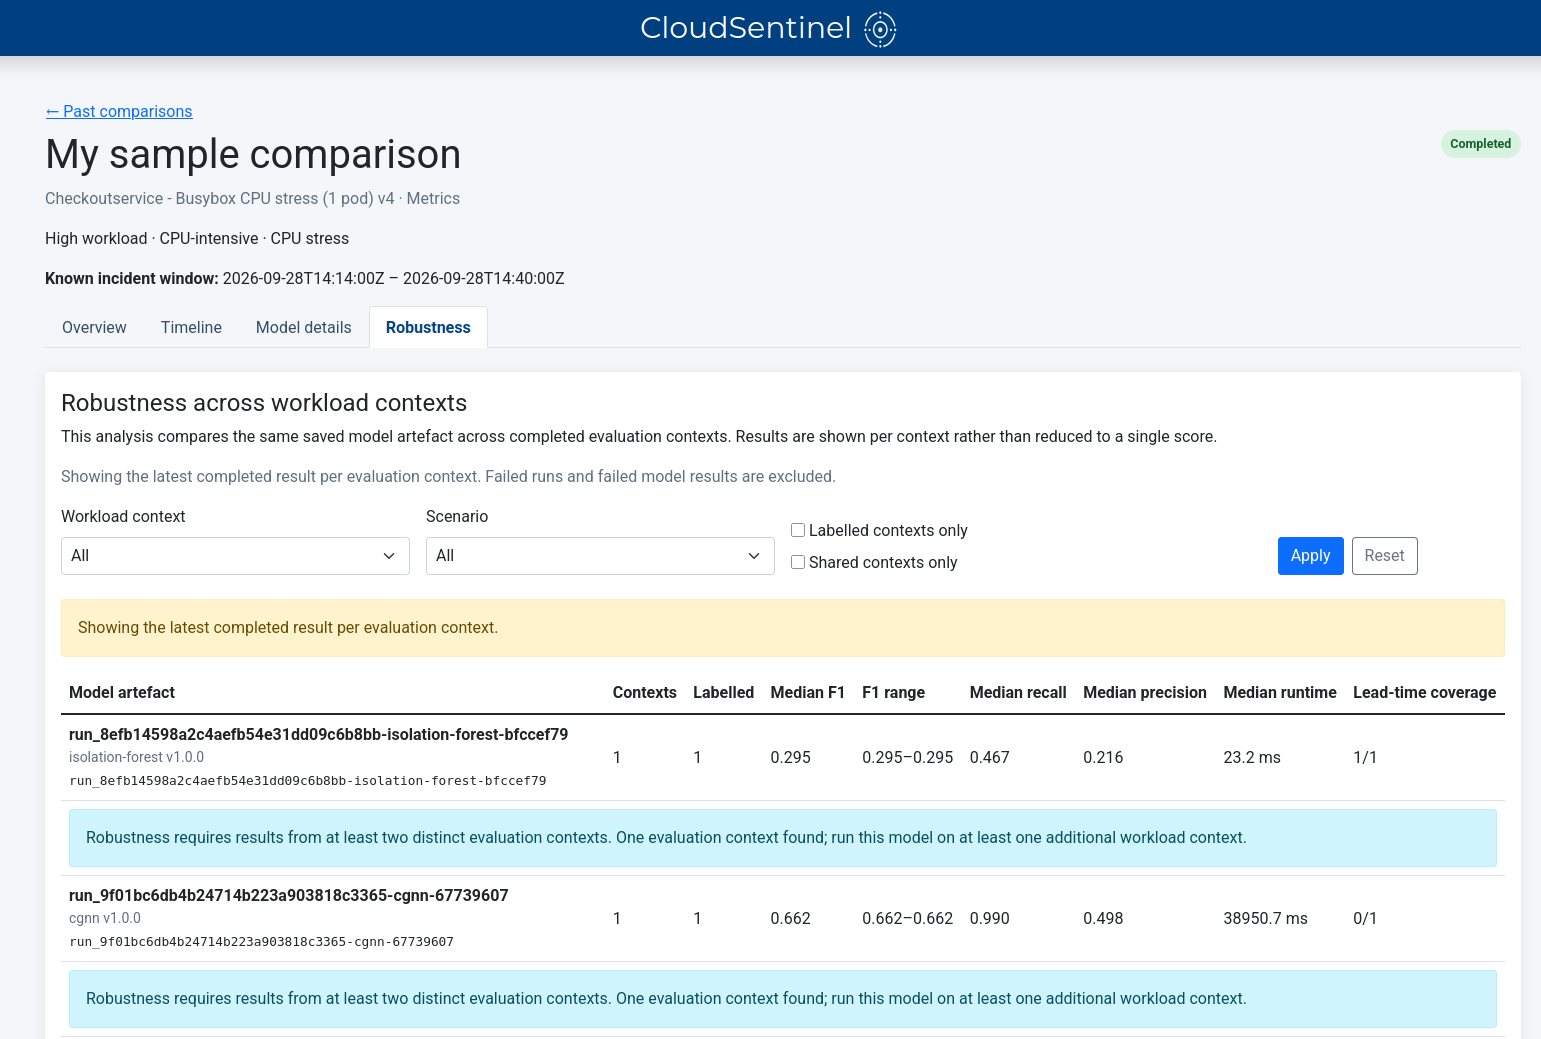
\includegraphics[width=1\linewidth]{figures/implementation/comparison/Screenshot from 2026-10-06 17-47-48.png}
    \caption{Historical robustness view for exact Saved Model artefacts across stored workload contexts.}
    \label{fig:comparison_robustness}
\end{figure}

The view can filter by workload intensity, anomaly scenario, labelled contexts only, and contexts shared by multiple selected artefacts. Below the summary, it presents the shared-context matrix and the retained historical context rows. Every row links back to its source ComparisonRun. Robustness is calculated read-only when requested; it does not rerun inference or rewrite earlier records. Responses are bounded to a configurable maximum number of contexts per model.

\subsubsection{Decision support and continued evaluation}

The first comparison interface presented the measured values but still left the operator to translate them into an operational choice. A later extension adds goal-based decision support without changing the stored ComparisonRun. The operator can select one of five goals: balanced detection, catching as many labelled incidents as possible, limiting false alarms, detecting an incident as early as possible, or limiting inference cost. These goals map respectively to F1, recall, precision, valid detection lead time, and measured inference runtime. Runtime is only a practical compute-cost proxy; it is not a measurement of financial cost or total cluster use.

For the selected goal, the Django layer reads the completed model results and identifies the best measured value among results for which that metric is available. Higher values are preferred for F1, recall, precision, and lead time, while lower runtime is preferred. Equal values remain a tie. Missing ground truth, a detection after incident start, and failed model results are excluded instead of being replaced by zero. The recommendation is deterministic and read-only: it neither changes the ComparisonRun nor activates a model. The interface explicitly states that the outcome applies only to the selected evaluation dataset and workload context. Figure~\ref{fig:comparison_decision_support} reserves the screenshot position for this view.

\begin{figure}[H]
    \centering
    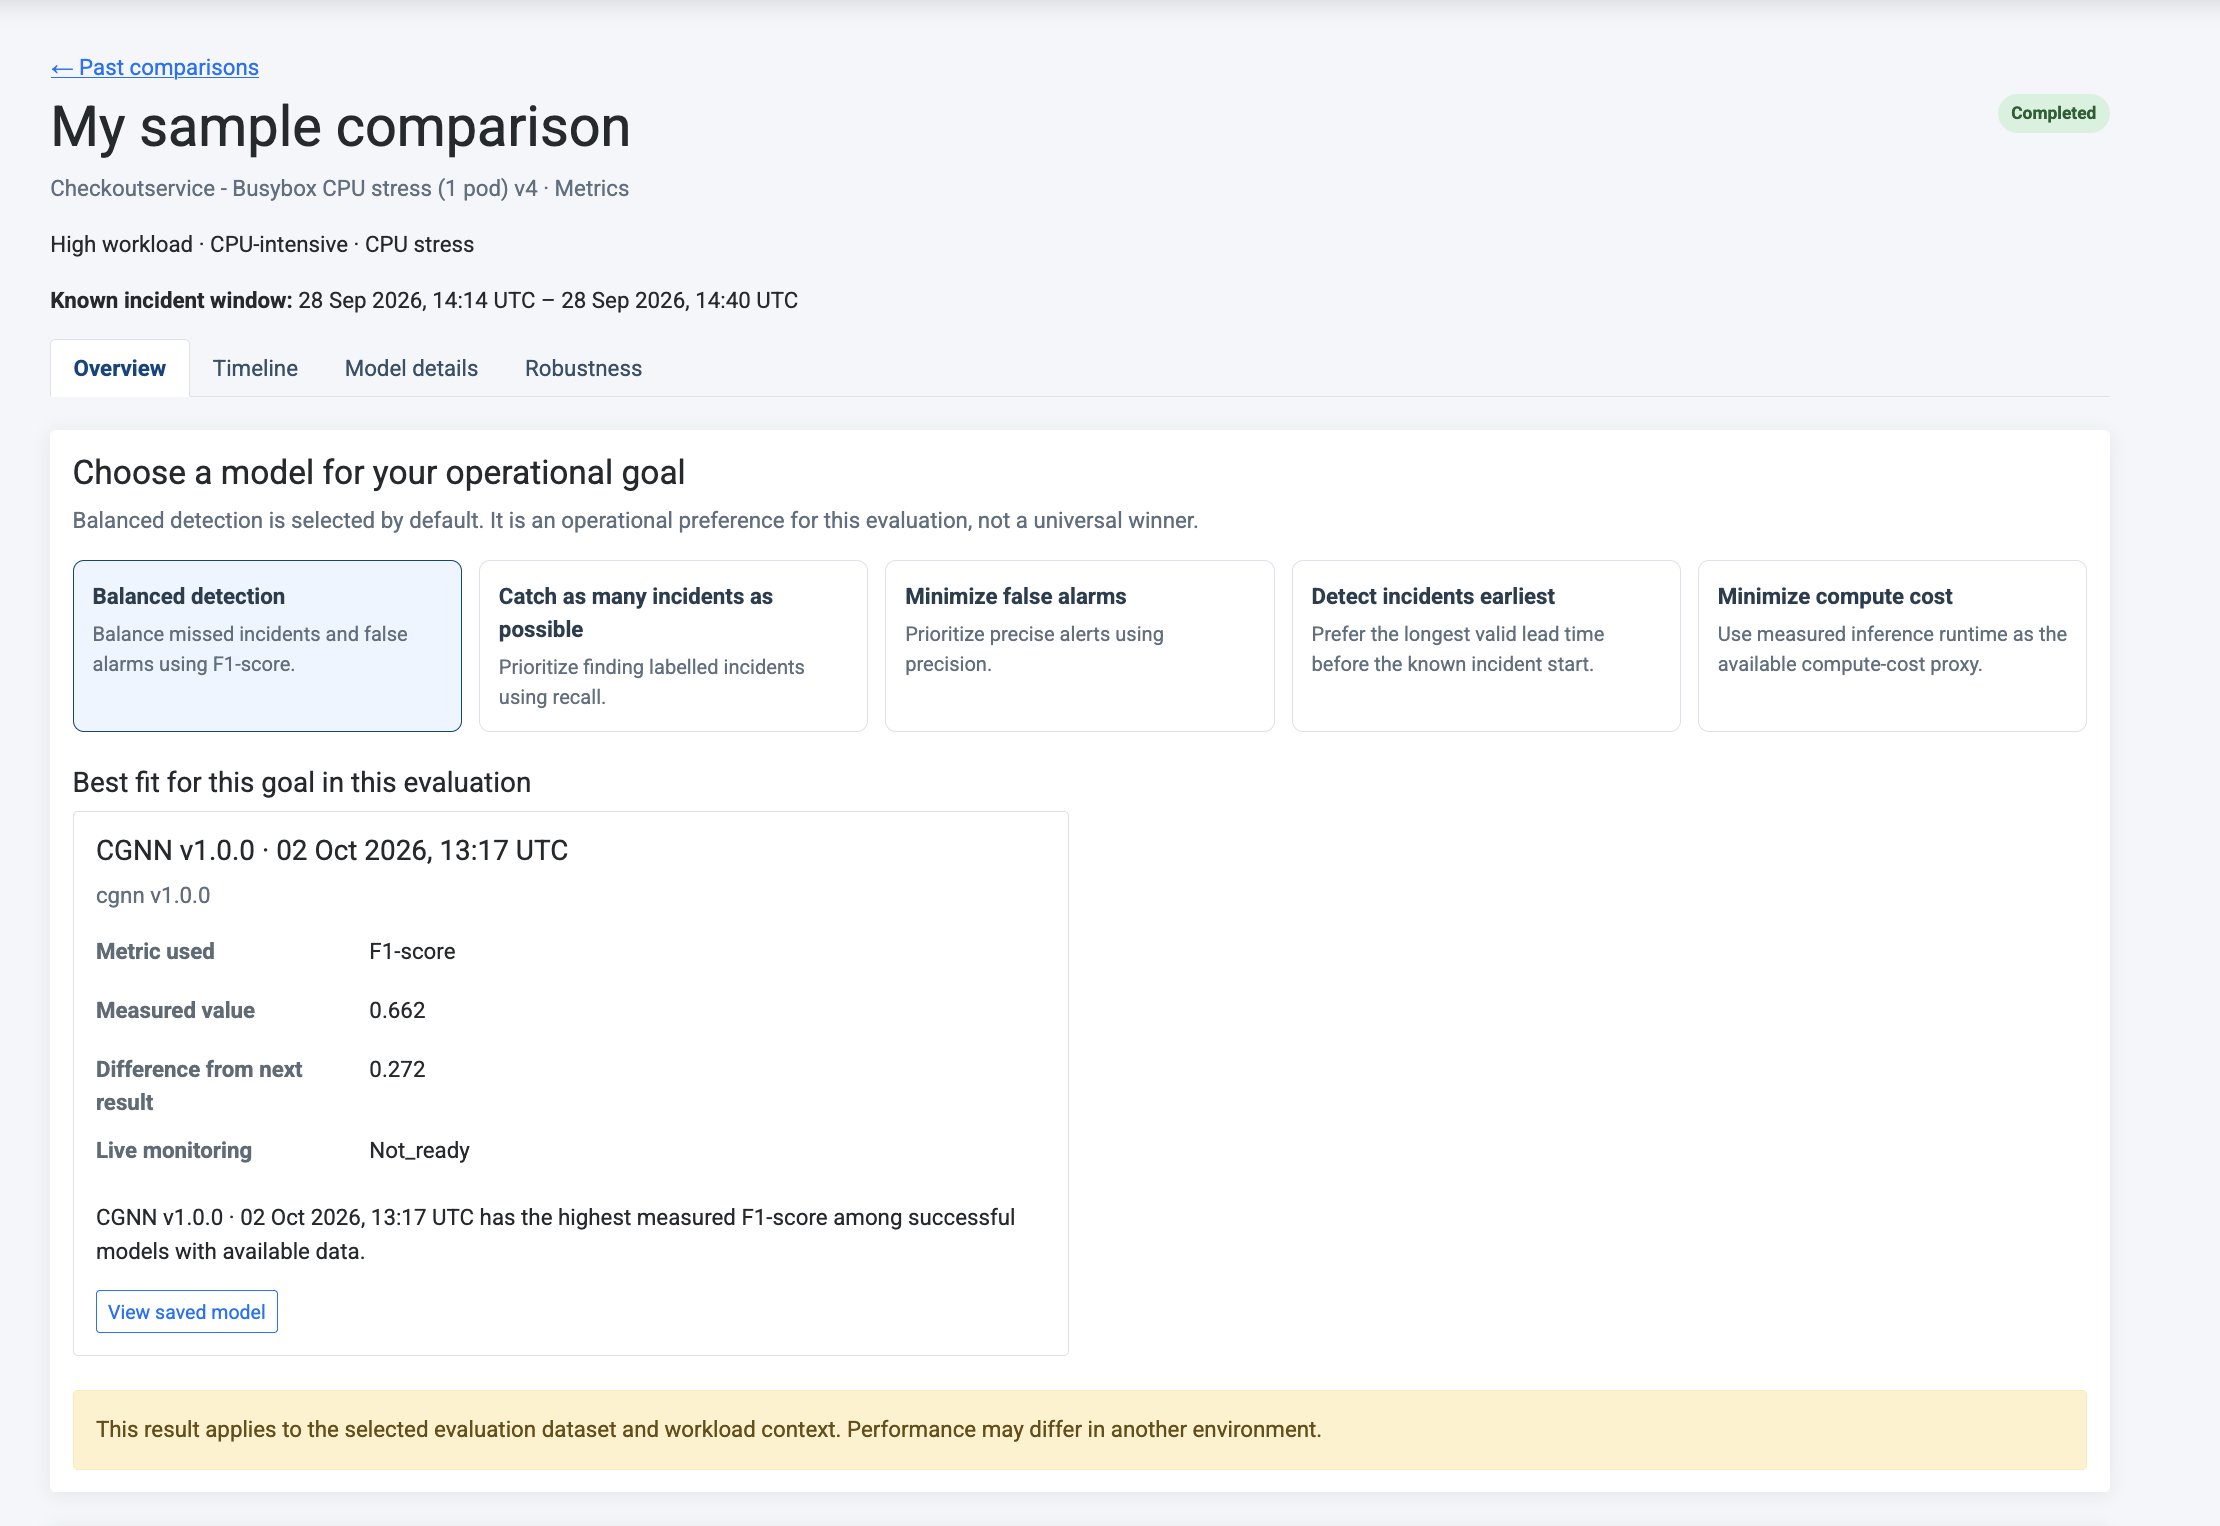
\includegraphics[width=1\linewidth]{figures/implementation/extra/Screenshot 2026-10-18 at 23.11.48.png}
    \caption{Goal-based decision support over the completed results of one shared evaluation context.}
    \label{fig:comparison_decision_support}
\end{figure}

The surrounding workflow was also connected more directly. A completed training run offers a comparison action when at least two children produced available models. Their identifiers are resolved on the server and preselected in the normal comparison wizard, but compatibility is checked again after the user selects an evaluation dataset. In the other direction, the Robustness tab can start a new comparison with the same exact model artefacts. This supports evaluating them in another workload context without manually finding every model again. Selecting the exact source partition produces a warning because it replaces the canonical repeated result rather than adding independent robustness evidence. The resulting continuation action is shown in Figure~\ref{fig:comparison_continued_context}.

The robustness summary was made more careful at the same time. It now reports the lowest labelled F1 context of each model in addition to coverage, medians, ranges, and runtime statistics. A direct statement about the lowest observed F1 variation is made only when every selected artefact has a successful, finite F1 result in at least two of the same immutable contexts. Ties remain ties, and results measured on different context sets are not used for this conclusion. This is still not a general robustness winner or a combined score.

Workload context remains operator-supplied metadata. CloudSentinel uses fixed categories for workload intensity, dominant workload characteristic, and anomaly scenario so that filtering and aggregation remain consistent. When the scenario \emph{Other} is selected, the user must provide a short custom description. CloudSentinel stores that detail but does not infer or validate that the description matches the collected measurements. Dataset context also remains separate from the exact incident windows used as ground truth.

\begin{figure}[H]
    \centering
    \IfFileExists{figures/implementation/comparison/continued_context_evaluation.png}{%
        \includegraphics[width=1\linewidth]{figures/implementation/comparison/continued_context_evaluation.png}%
    }{%
        \fbox{\parbox[c][55mm][c]{0.92\linewidth}{\centering
        TODO: Add screenshot of Comparison result $\rightarrow$ Robustness.\\
        Also show shared contexts and the action ``Evaluate these models in another context''.}}%
    }
    \caption{Continued evaluation of the same immutable model artefacts across additional workload contexts.}
    \label{fig:comparison_continued_context}
\end{figure}

\subsubsection{Deployment and implementation boundaries}

Comparison execution runs in the learning-adaptation Celery worker and uses the same server-configured Data Catalogue and Generic Detection Runtime endpoints as the surrounding pipeline. Comparison records reside on shared learning storage so that the API and worker observe the same state and completed results remain readable after process restarts. The Django service only proxies safe API projections. The deployment assumes one active learning worker for the staging queue used in this study; an outdated worker on the same queue could otherwise consume a task it cannot execute.

The storage and robustness scan are file-backed. Process locks and atomic replacement are suitable for the current shared single-node environment, but a larger multi-node deployment would benefit from a database, distributed locking, and indexed robustness queries. Robustness is calculated on demand and capped rather than cached. One comparison task evaluates models sequentially, so increasing the selected model count increases task duration.

The implemented scope has several functional limits. Only the active explicit partition is offered; timeline values are sampled; detector score scales are not calibrated against each other; and comparison cancellation, deletion, export, RCA, remediation, and automatic operational actions are not provided. Historical robustness also remains limited to anomaly detection and to records with complete immutable artifact and partition identity.

\subsubsection{Resulting workflow}

The implemented workflow begins with one available Data Catalogue partition and at least two inference-ready Saved Models. CloudSentinel checks modality, feature identity, inference contract, and artefact evidence; records the exact dataset and artefact identities; and dispatches one comparison task. The worker verifies the evaluation bundle, activates and evaluates each immutable model, checks runtime output and artefact identity, calculates available metrics and detection timing, bounds the timeline, and persists each model result independently.

The final ComparisonRun can be revisited through its overview, timeline, model, experiment-evidence, and robustness views. Later comparisons of the same exact model artefact on other workload contexts become historical robustness evidence without altering the original records. The component therefore completes a traceable chain from collected evaluation data, through trained model artefacts, to context-specific and cross-context performance evidence.

\subsection{Revised Live Monitoring and Monitoring History}

Live monitoring had to be revised as a consequence of the new dataset, plugin, and Saved Model contracts. The earlier monitoring path called CGNN-specific preprocessing and detection endpoints and selected a detector configuration indirectly. The revised implementation instead selects one exact Saved Model and uses its pinned input and inference contracts. This was required to make the features described above usable after training rather than only in offline comparisons.

During implementation, the monitoring result was also changed from a short-lived task response into a durable session history. This second change was not fully described in the initial design. It was added because an operator must be able to revisit which model was active, which observations were evaluated, and when an anomaly value was produced. Redis remains useful for temporary execution state, but is not treated as the long-term record.

\subsubsection{Architecture and live-input contract}

Figure~\ref{fig:live_monitoring_architecture} shows the implemented path. The Django interface starts and reads sessions through the Data Ingestion API. Data Ingestion obtains the selected model's safe live-monitoring information from the Learning service, collects observations from the server-configured Prometheus source, and calls the Generic Detection Runtime. The selected detector adapter loads the exact model artefact and applies the preprocessing stored during training. Completed cycle summaries and private evidence are committed to monitoring-history storage before they appear in the interface.

\begin{figure}[H]
    \centering
    \resizebox{0.98\linewidth}{!}{%
    \begin{tikzpicture}[
        font=\small,
        node distance=10mm and 11mm,
        component/.style={draw, rounded corners=2pt, align=center, minimum height=11mm, text width=27mm, fill=blue!7},
        external/.style={draw, rounded corners=2pt, align=center, minimum height=11mm, text width=25mm, fill=orange!11},
        storage/.style={draw, cylinder, shape border rotate=90, aspect=0.25, align=center, minimum height=14mm, text width=28mm, fill=green!10},
        flow/.style={-{Latex[length=2mm]}, thick},
        evidence/.style={-{Latex[length=2mm]}, thick, dashed}
    ]
        \node[component] (ui) {Monitoring Setup and History UI};
        \node[component, right=of ui] (ingestion) {Data Ingestion API and worker};
        \node[external, right=of ingestion] (prometheus) {Configured Prometheus source};
        \node[component, below=18mm of prometheus] (runtime) {Generic Detection Runtime};
        \node[component, below=16mm of ui] (learning) {Learning service and Saved Model};
        \node[storage, below=18mm of ingestion] (history) {Durable sessions, cycles, and artefacts};

        \draw[flow] (ui) -- (ingestion);
        \draw[flow] (ingestion) -- node[above, font=\scriptsize] {fixed queries} (prometheus);
        \draw[flow] (prometheus) to[bend left=15] node[below, font=\scriptsize] {time series} (ingestion);
        \draw[flow] (learning) -- node[left, font=\scriptsize] {model and recipe identity} (ingestion);
        \draw[flow] (ingestion) -- node[right, font=\scriptsize] {verified matrix} (runtime);
        \draw[evidence] (runtime) -- node[below, font=\scriptsize] {predictions and scores} (history);
        \draw[flow] (ingestion) -- (history);
        \draw[flow] (history) -- (ui);
    \end{tikzpicture}%
    }
    \caption{Revised live-monitoring architecture using an explicit Saved Model, reproducible live input, generic inference, and durable history.}
    \label{fig:live_monitoring_architecture}
\end{figure}

A newly fetched Prometheus-backed catalogue version contains an immutable \texttt{cloudsentinel.live-input/v1} recipe. The recipe records the Prometheus source identifier, resolved query executions, target bindings, exact series-to-feature mapping, sampling interval, timestamp alignment, feature order, and missing-value policy. Its canonical checksum and feature-order hash are carried through the training snapshot into the Saved Model record. This connects the model not only to its training values, but also to the instructions needed to collect compatible live values.

Only models with a complete and valid recipe are marked live-ready. Older models remain valid for offline inference and comparison, but CloudSentinel does not guess live PromQL from their feature names. When a session is created, Data Ingestion resolves the selected model again and pins the model ID, artefact-manifest hash, recipe hash, and feature-order hash. A later model or catalogue change therefore cannot silently alter an active session.

The monitoring worker executes only the stored queries against the configured Prometheus source and rebuilds columns through the same canonical series-mapping logic used during catalogue collection. Off-grid samples are ignored with a warning. A live window containing a missing value is rejected rather than filled or interpolated, because invented values could change a detector result. The assembled matrix and its feature identity are sent once to the Generic Detection Runtime. Detector-specific scaling, sequence construction, warm-up, and prediction remain the responsibility of the pinned adapter.

\subsubsection{Session cycles and durable history}

A monitoring session stores a display name, model and detector identity, recipe and artefact hashes, window and polling configuration, lifecycle timestamps, and a copy of the immutable recipe. Each worker invocation creates a separate cycle. Durable files are stored below the existing Data Catalogue persistent volume, while Redis contains only temporary execution state and the bounded buffer used by the active task.

The implementation distinguishes four times. The \emph{query window} is the period requested from Prometheus. The \emph{inference window} is the bounded context sent to the model. The \emph{prediction window} contains only prediction timestamps that have not been committed previously. Processing time records when collection, inference, and storage took place. Keeping these concepts separate is especially important for sequence models: an inference window may repeat older observations as context even though only its newest predictions belong to the new cycle.

Each session therefore has a prediction watermark. On the first successful cycle, every aligned prediction is eligible. Later cycles accept only timestamps strictly newer than the committed watermark. The watermark advances only after the input, result, and cycle record have been written successfully. A retry with the same deterministic cycle identifier reuses the stored cycle. Overlapping Prometheus windows and task retries consequently do not count the same prediction twice.

The displayed anomaly percentage is calculated as the number of anomalous predictions divided by the number of newly eligible predictions in that cycle. The complete context-buffer length is not used as the denominator. When a detector is still warming up, or when no prediction is newer than the watermark, the percentage is unavailable. The interface shows \emph{warm-up} or \emph{no new data} instead of incorrectly displaying zero percent.

Private cycle input and output are stored as checksummed, content-addressed JSON artefacts. A cycle record refers to these artefacts and contains bounded summaries. This means that old monitoring evidence remains available even after the corresponding Prometheus samples have expired. Public API responses omit matrices, PromQL, complete predictions and scores, filesystem paths, task identifiers, internal URLs, and stack traces.

\subsubsection{Monitoring interface and lifecycle}

The setup screen in Figure~\ref{fig:monitoring_setup} presents three ordered decisions: the session and exact Saved Model, the detection window and poll interval, and optional RCA. The side panel explains whether each model is live-ready and whether its input is suitable for RCA. Detailed reanalysis limits remain available as advanced settings instead of occupying the main path. Direct Grafana and Prometheus links allow the researcher to inspect telemetry that is not reproduced in CloudSentinel. Monitoring does not start merely by opening a model or comparison result; the user must still submit the setup form.

\begin{figure}[H]
    \centering
    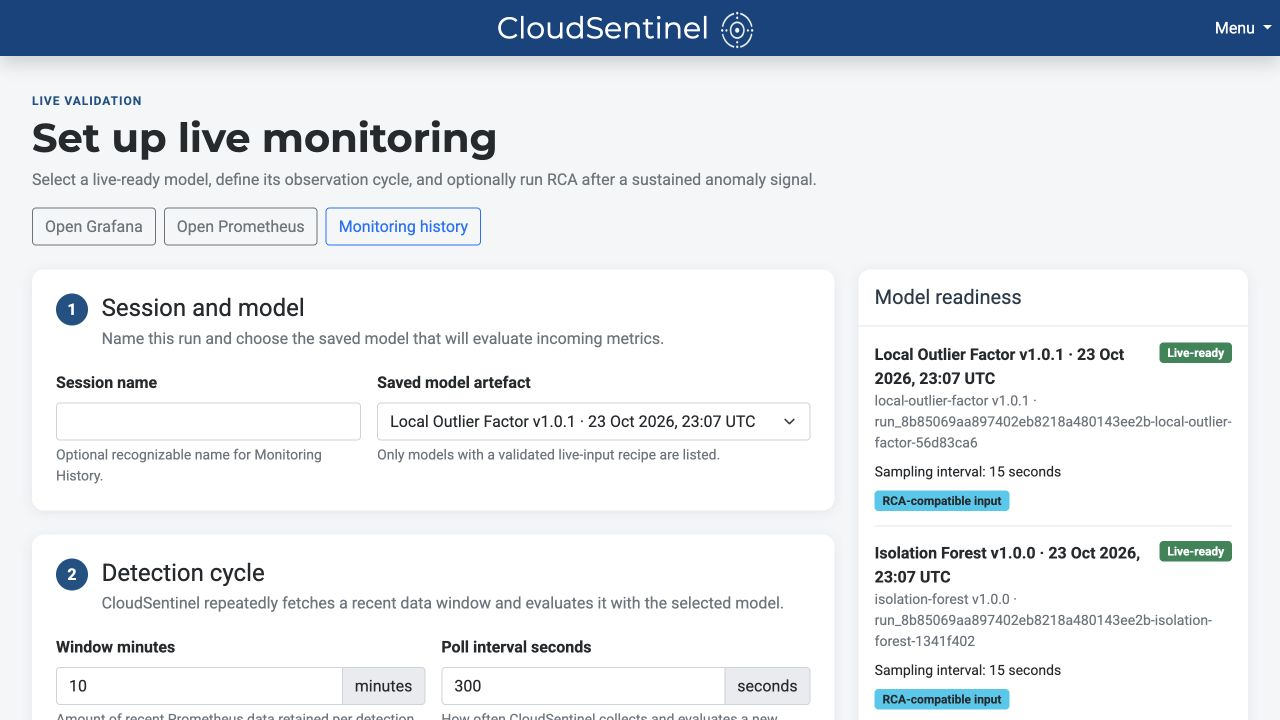
\includegraphics[width=1\linewidth]{figures/implementation/current/monitoring_setup.jpg}
    \caption{Three-step Monitoring Setup with exact model selection, detection-cycle settings, optional RCA, and model-readiness information.}
    \label{fig:monitoring_setup}
\end{figure}

Monitoring History uses a master-detail layout, shown in Figure~\ref{fig:monitoring_history}. The selected session remains addressable through its identifier and can be revisited after a page refresh. Its detail shows lifecycle state, model provenance, timing configuration, committed cycle summaries, warnings, and a chart containing one point for each cycle with a valid percentage. Polling updates the existing view only when the safe response changes and pauses while the page is hidden.

% \begin{figure}[H]
%     \centering
%     \IfFileExists{figures/implementation/live_monitoring/monitoring_history.png}{%
%         \includegraphics[width=1\linewidth]{figures/implementation/live_monitoring/monitoring_history.png}%
%     }{%
%         \fbox{\parbox[c][55mm][c]{0.92\linewidth}{\centering
%         Screenshot to add: Monitoring History.\\
%         Show the session list, selected session, lifecycle status, chart, and recent committed cycles.}}%
%     }
%     \caption{Durable Monitoring History containing live and completed sessions with bounded cycle summaries.}
%     \label{fig:monitoring_history}
% \end{figure}

\begin{figure}[H]
    \centering
    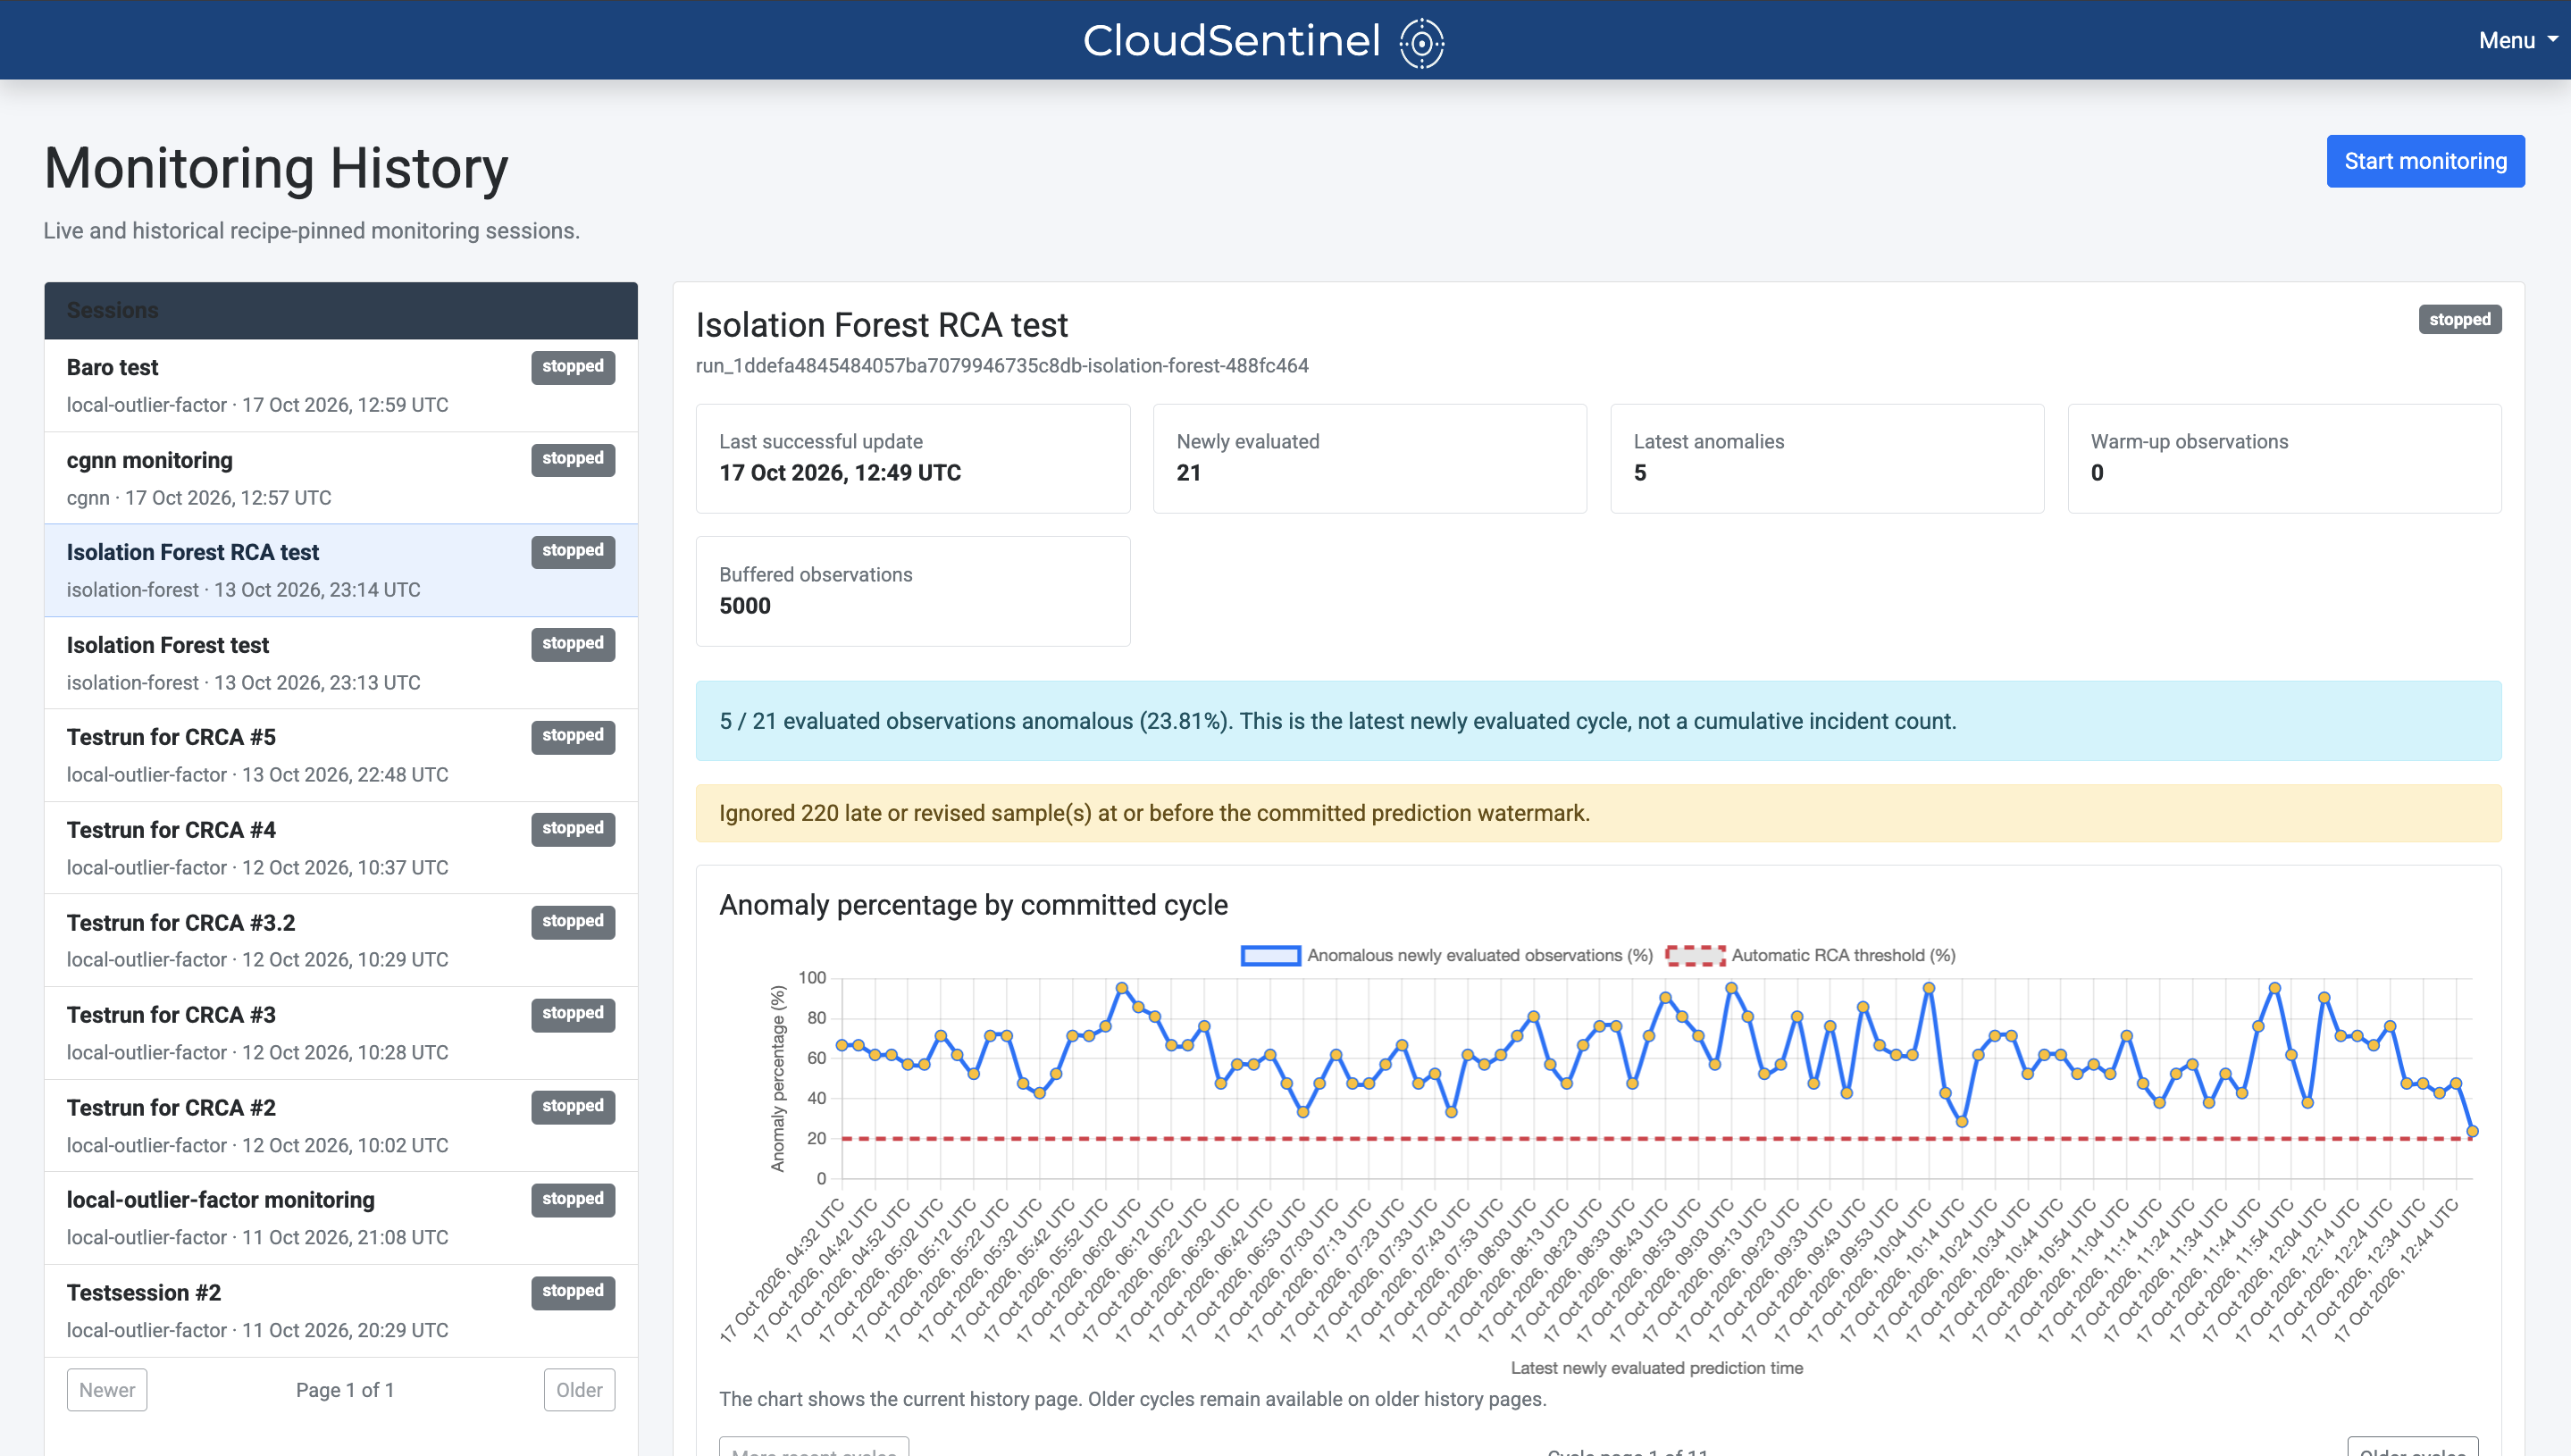
\includegraphics[width=1\linewidth]{figures/implementation/extra/Screenshot 2026-10-18 at 23.17.08.png}
    \caption{Durable Monitoring History containing live and completed sessions with bounded cycle summaries.}
    \label{fig:monitoring_history}
\end{figure}

Stopping a session is written to durable storage before task revocation is attempted. A worker that completes late cannot publish another cycle after that stop. History remains readable when Redis state expires or is lost; a session that was active but has no execution state is shown as interrupted and is not resumed automatically. Failed collection or inference creates a safe failed state without deleting earlier cycles.

The file-backed history matches the study's single-node deployment but has clear limits. Input and result artefacts increase storage use, and no automatic retention or orphan cleanup is currently implemented. The API and worker rely on a shared filesystem and process-level locks. A larger multi-node deployment would require coordinated storage, distributed locking, and an explicit retention policy.

\subsection{Automatic and Selectable Root-Cause Analysis}

The baseline framework contained CausalRCA, but the new generic monitoring route initially had no reliable way to supply it with detector-independent input and provenance. Automatic RCA was therefore reconnected after durable monitoring cycles were available. It was subsequently extended with explicit method selection and bounded reanalysis. These additions were made during implementation rather than being fully defined in the original interface design.

Anomaly detection and RCA remain separate. A model can be live-ready while its recipe is not suitable for RCA, and an RCA failure never stops the anomaly-detection session. Automatic RCA is disabled by default and must be enabled when a new monitoring session is configured.

\subsubsection{Trigger and episode control}

The trigger is based on a successfully committed monitoring cycle. An RCA intent is considered only when that cycle has newly eligible predictions and its anomaly percentage is strictly greater than the configured threshold. Equality does not trigger. Warm-up and no-new-data cycles have no percentage and therefore neither trigger an analysis nor count as recovery.

Figure~\ref{fig:monitoring_rca_pipeline} summarises the path. Data Ingestion selects an RCA analysis window from the exact checksummed input of the triggering cycle. It does not query Prometheus again. The selected method, model and recipe identities, configuration, analysis window, and input checksum form a stable run identity. The CRCA worker then executes the pinned method adapter and stores a validated ranking and, where supported, a graph.

\begin{figure}[H]
    \centering
    \resizebox{0.98\linewidth}{!}{%
    \begin{tikzpicture}[
        font=\small,
        node distance=8mm,
        processstep/.style={draw, rounded corners=2pt, align=center, minimum height=11mm, text width=27mm, fill=blue!7},
        decision/.style={draw, diamond, aspect=2.1, align=center, inner sep=1.5pt, text width=25mm, fill=orange!11},
        result/.style={draw, rounded corners=2pt, align=center, minimum height=11mm, text width=29mm, fill=green!10},
        flow/.style={-{Latex[length=2mm]}, thick}
    ]
        \node[processstep] (cycle) {Committed monitoring cycle};
        \node[decision, right=of cycle] (trigger) {New predictions and above threshold?};
        \node[processstep, right=of trigger] (input) {Select checksummed RCA window};
        \node[processstep, below=15mm of input, xshift=-24mm] (method) {Validate and pin selected RCA method};
        \node[processstep, below=15mm of input, xshift=24mm] (execute) {Execute method adapter in CRCA worker};
        \node[result, right=of execute] (store) {Store bounded ranking, graph, and provenance};
        \node[result, below=15mm of trigger] (suppress) {No run: recovered, suppressed, or preflight skipped};

        \draw[flow] (cycle) -- (trigger);
        \draw[flow] (trigger) -- node[above, font=\scriptsize] {yes} (input);
        \draw[flow] (trigger) -- node[left, font=\scriptsize] {no} (suppress);
        \draw[flow] (input) -- (method);
        \draw[flow] (method) -- (execute);
        \draw[flow] (execute) -- (store);
    \end{tikzpicture}%
    }
    \caption{Monitoring-triggered RCA uses already committed evidence and a pinned method contract.}
    \label{fig:monitoring_rca_pipeline}
\end{figure}

The session keeps episode state to prevent a continuously high anomaly percentage from creating an unbounded number of tasks. The first accepted threshold crossing creates one durable intent. Continued high cycles are normally marked as belonging to the same episode. A cycle at or below the threshold records recovery, while a configurable cooldown controls when a later episode may start.

An operator can optionally enable same-episode reanalysis. A later high cycle is accepted only when no run is active, a minimum interval has passed, enough new timestamps exist beyond the previous analysis end, the selected content has changed, and the configured attempt budget has not been exhausted. These checks use server timestamps and unique observation timestamps rather than browser polling or buffer length. An input-selection problem is stored as a preflight skip; it does not consume an execution attempt.

\subsubsection{Selectable RCA methods}

The monitoring setup retrieves the available RCA methods from the CRCA service. Data Ingestion validates the chosen method during session creation and stores its identifier and configuration digest. The worker checks these values again before execution. Existing records without an explicit method remain compatible and resolve to the earlier CausalRCA implementation; an unknown explicit identifier is never silently replaced.

\begin{table}[H]
    \centering
    \caption{Implemented monitoring RCA methods and their different contracts.}
    \label{tab:monitoring_rca_methods}
    \resizebox{\linewidth}{!}{%
    \begin{tabular}{@{}p{34mm}p{45mm}p{51mm}p{43mm}@{}}
        \toprule
        \textbf{Method} & \textbf{Input interpretation} & \textbf{Preprocessing} & \textbf{Stored result} \\
        \midrule
        CausalRCA & Finite multivariate observations from the selected monitoring window & Per-column MinMax transformation pinned for the RCA run & Ranked features and, when produced, a dependency graph \\
        BARO RobustScorer & Baseline and anomalous segments around a detector-derived change point & Finite raw metric values; robust baseline normalisation inside RobustScorer & Ranked features and change-point evidence; no causal graph \\
        \bottomrule
    \end{tabular}%
    }
\end{table}

CausalRCA keeps the preprocessing and algorithm used by the earlier CloudSentinel component, but receives explicit feature identities and an immutable input window. BARO uses the pinned \texttt{fse-baro} RobustScorer implementation. It does not run BARO's own change-point detector. Instead, CloudSentinel takes the first positive anomaly prediction stored inside the selected RCA window. Rows before that index form the baseline and rows at and after it form the anomalous segment. The timestamp, matrix index, source cycle, and segment sizes are retained as evidence. A missing positive prediction or too few observations on either side produces a preflight skip.

Both methods retain the exact feature ID as the matrix-column identity. Optional pod or service information is used only when it was explicitly captured in the live-input recipe; it is not parsed from PromQL or guessed from a feature name. CausalRCA may produce a dependency graph, whereas BARO returns an ordering based on robust changes and deliberately produces no graph. Scores are relative within one run and are not probabilities or values that can be compared directly between the two methods.

\subsubsection{Persistence and interface}

For every accepted analysis, Data Ingestion first writes a durable RCA intent. It then dispatches only the session and stable run identifier to the CRCA service. The worker reads the private checksummed input, atomically claims the run, executes the pinned adapter, validates its output, and writes a checksummed result. A dispatch failure leaves the intent available for a controlled retry. An execution failure is stored on that run and cannot reactivate, stop, or otherwise change the monitoring session.

Monitoring History displays the configured method, threshold and windows, trigger decision, attempt number, lifecycle state, bounded feature ranking, optional graph, and safe provenance. Suppressed, skipped, failed, and completed analyses remain distinguishable. Figure~\ref{fig:monitoring_rca_result_1} reserves one screenshot for this combined result view rather than requiring a separate image for every lifecycle variant.

\begin{figure}[H]
    \centering
    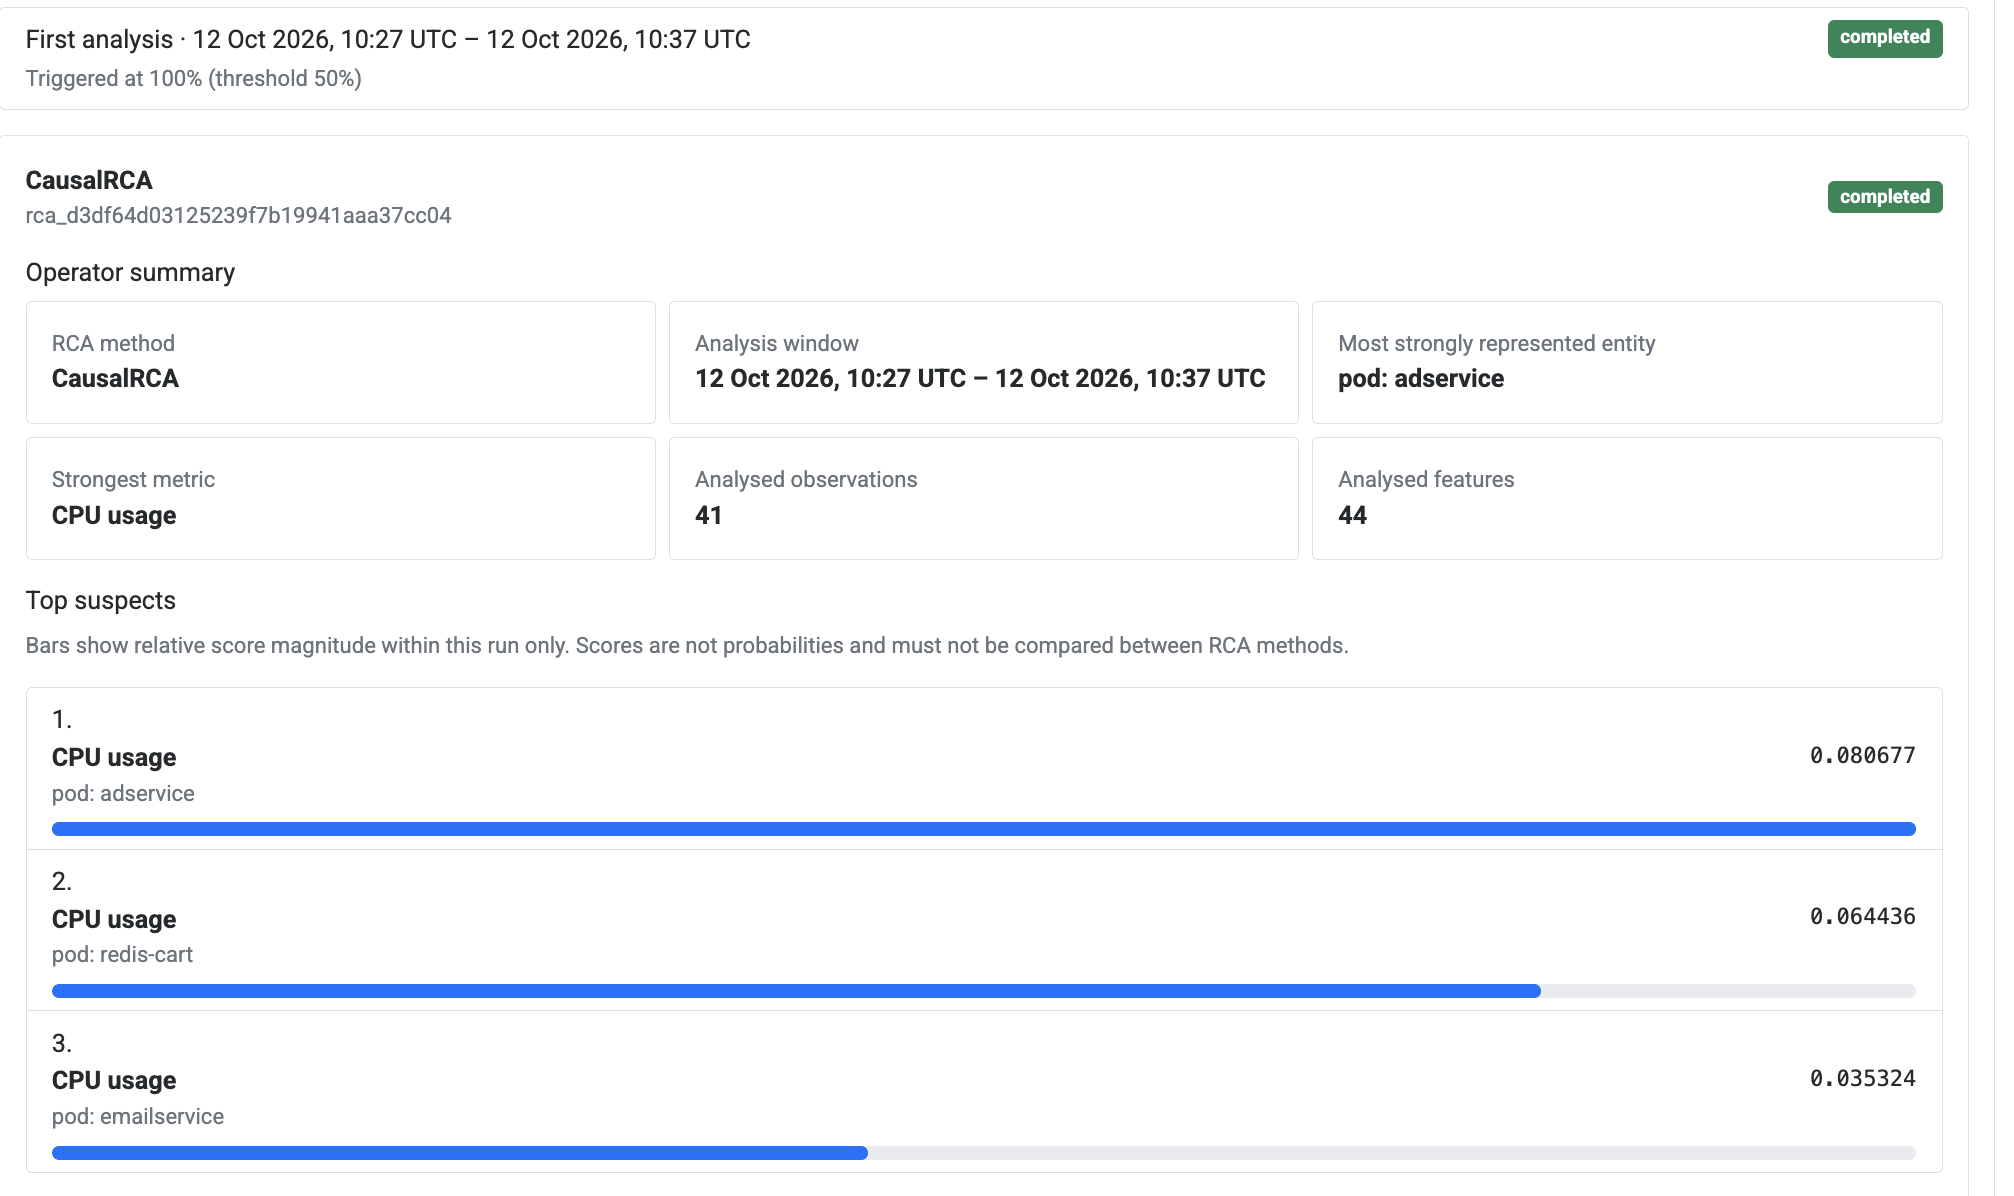
\includegraphics[width=1\linewidth]{figures/implementation/extra/Screenshot 2026-10-18 at 23.19.27.png}
    \caption{Stored RCA result within Monitoring History, including method identity.}
    \label{fig:monitoring_rca_result_1}
\end{figure}

\begin{figure}[H]
    \centering
    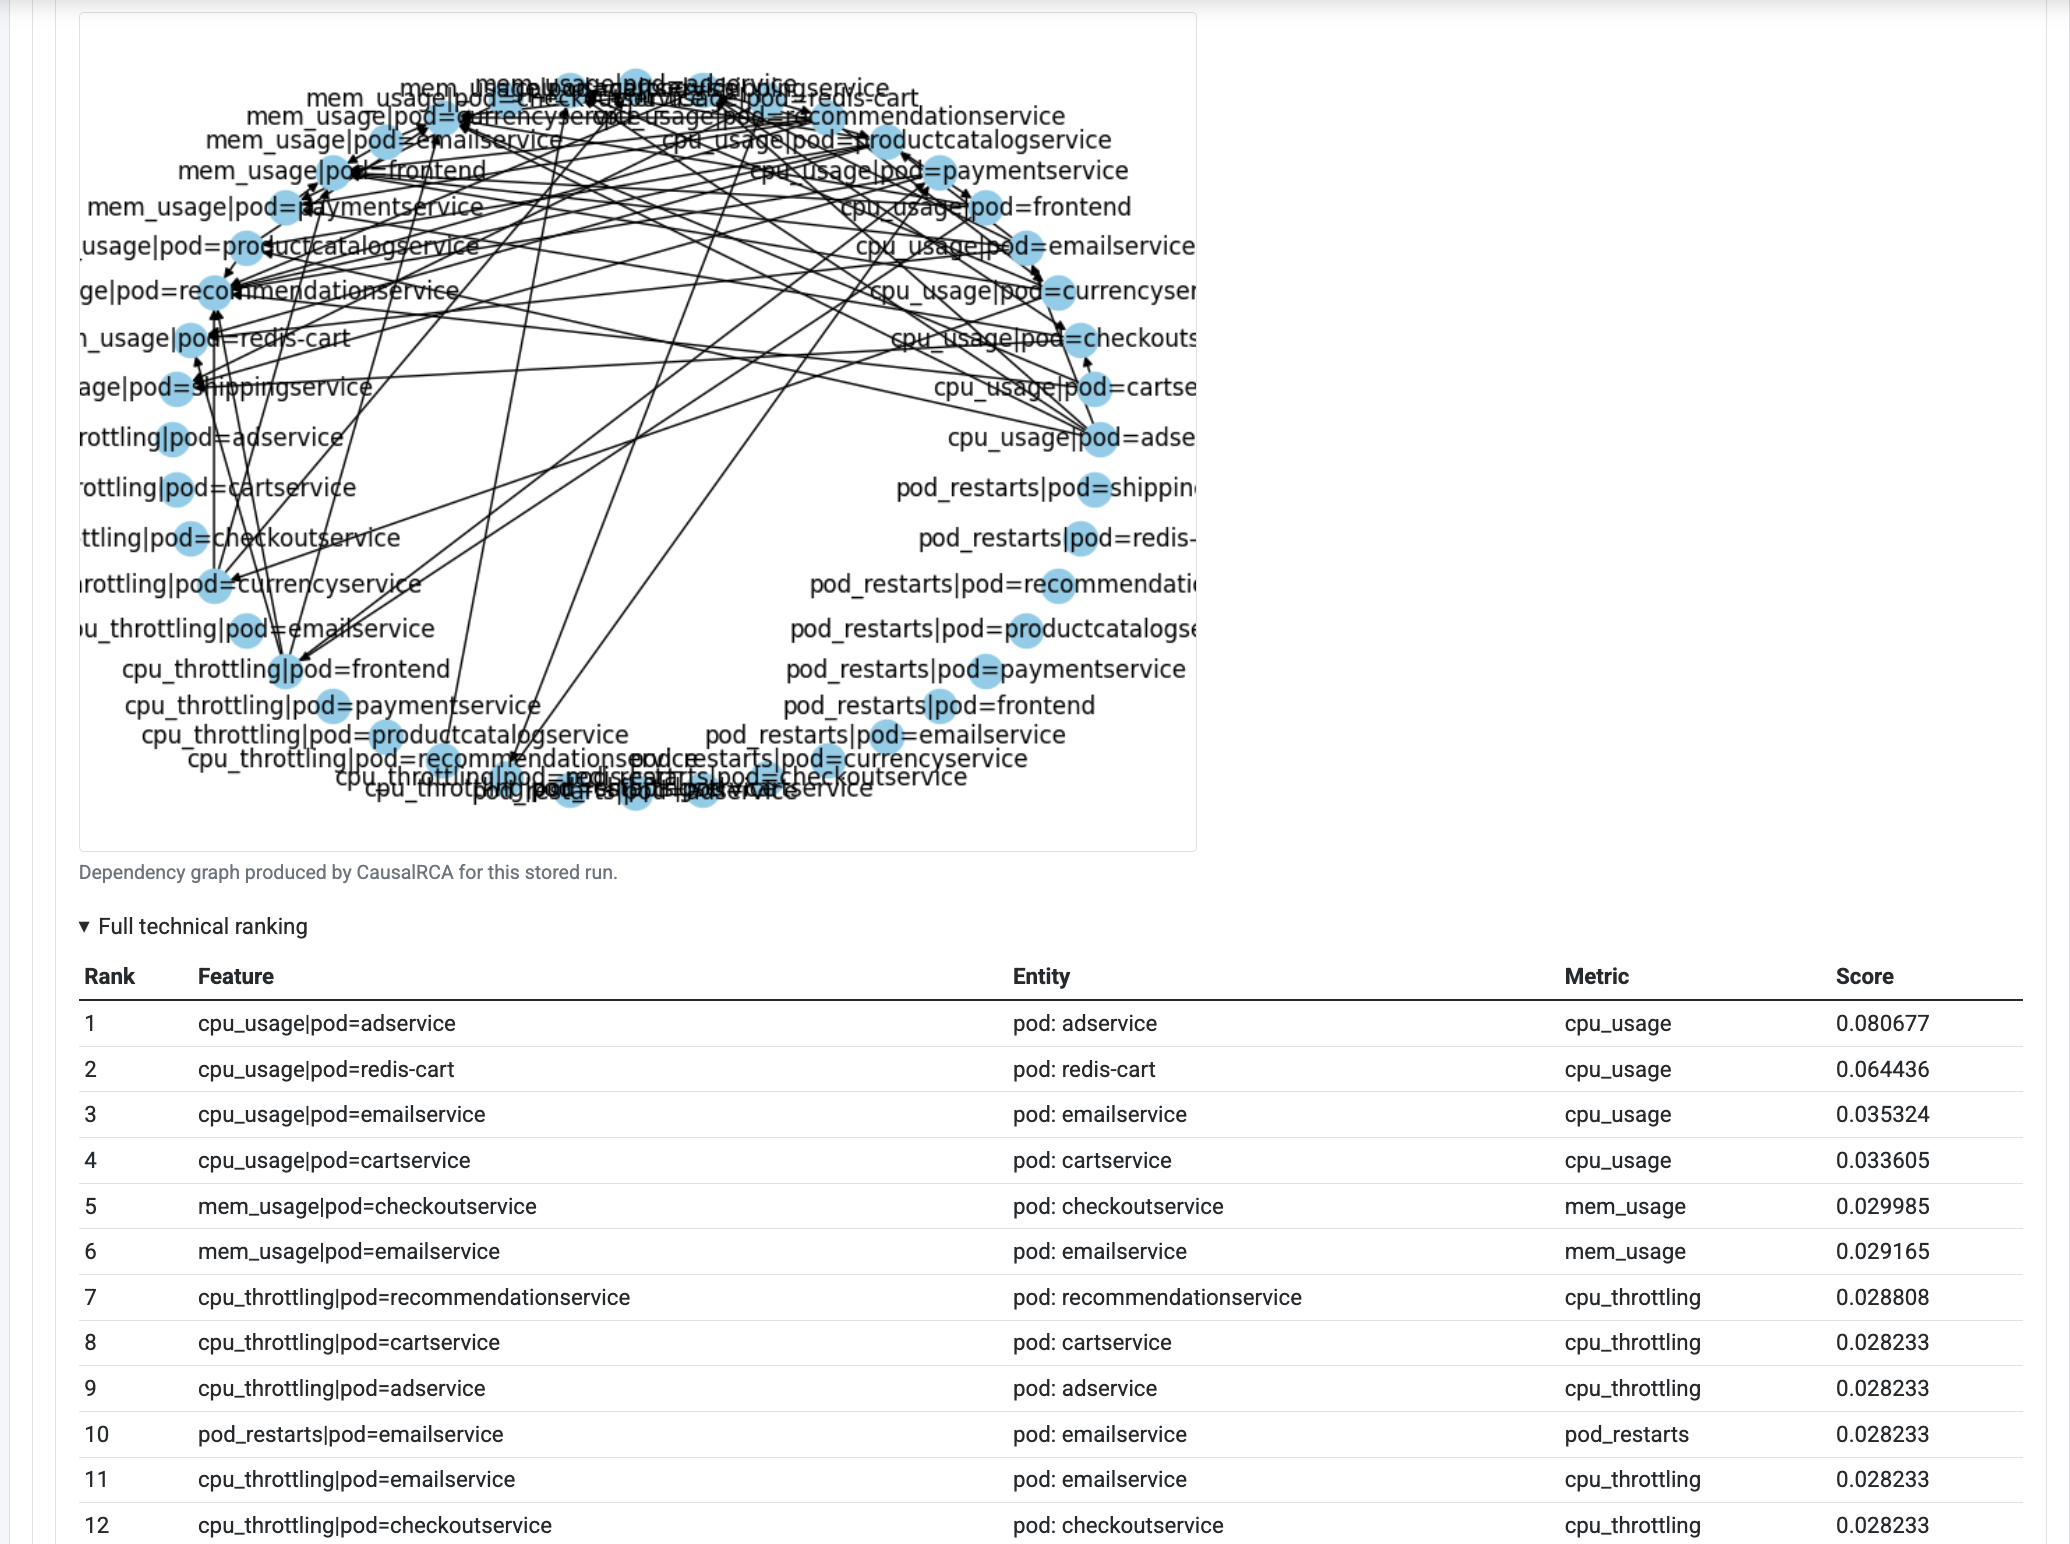
\includegraphics[width=1\linewidth]{figures/implementation/extra/Screenshot 2026-10-18 at 23.19.45.png}
    \caption{RCA bounded ranking and safe provenance.}
    \label{fig:monitoring_rca_result_2}
\end{figure}

The interface describes every ranking as diagnostic evidence. A high anomaly percentage does not by itself prove that an incident occurred, a top-ranked feature is not automatically the actual root cause, and a CausalRCA graph shows calculated dependencies rather than proven causality. These limits are important because the new pipeline improves repeatability and inspectability, but does not remove the need for operator interpretation.

The implementation reuses the existing monitoring-history volume and CRCA service. No separate RCA database was introduced. As with monitoring history, the current file-backed locks and shared volume suit the controlled single-node environment. There is no automatic retention for RCA matrices or graph files, and a worker that remains indefinitely in a running state still requires operator investigation rather than automatic duplicate execution.

% TEMPLATE VOOR SECTION 9.4
% Gewone tekst is voor de thesislezer. Comments zijn werktaken.
% Resultaten zijn nog niet ingevuld. Pas verleden tijd toe na uitvoering.
% Standaard LaTeX; geen extra packages nodig.

\section{Evaluation of the improvement}
\label{sec:improvement-evaluation}

\subsection{Objectives}

The evaluation checks whether the new functions work, what resources they use, and whether CloudSentinel can be used outside the controlled Boutique environment. It uses the five criteria from Section 5.5: C1 (end-to-end experimental workflow adequacy), C2 (RCA workflow adequacy and interpretability), C3 (portability and deployment ease), C4 (configurability, reproducibility, and extensibility), and C5 (operational overhead).

Five parts are included:
\begin{enumerate}
    \item Tests of dataset management, training, model comparison, and detector integration.
    \item Performance and resource-use measurements.
    \item Detection and RCA tests with known faults in Boutique.
    \item External benchmark validation in a second microservice environment.
    \item User evaluation.
\end{enumerate}

These parts answer different questions. For example, correctly calculating a model's score does not mean that the model detects every fault. Running RCA successfully does not mean that its diagnosis is correct.

\subsection{Setup and evidence}

The tests used the deployed version of CloudSentinel and Online Boutique on a single-node Minikube cluster hosted on EC2. The exact software version, container images, machine resources, queries, and test identifiers can be found in \texttt{evaluation\_evidence/setup.txt} for the sake of reproducibility.

Two catalogue datasets were used. The first contained a labelled CPU-stress period and was used for training and for checking the calculated scores. The second contained normal application activity and was used to see whether the same trained models behaved differently in another workload context. Both datasets contained the same 44 CPU, memory, CPU-throttling, and restart features for eleven Boutique pods, sampled every 15 seconds.

Three anomaly detector algorithms were included: the built-in CGNN and Isolation Forest detectors, and an externally installed Local Outlier Factor (LOF) detector. Every action was linked to a stored dataset, training run, model, or comparison record. The full settings and outputs can be found in \texttt{evaluation\_evidence}; the main text below focuses on what was tested, what happened, and why that result matters.

After the final workflow and navigation changes, a focused regression test was also performed. All 116 selected backend tests and all 91 selected deployed-interface tests passed. A deployed smoke check returned HTTP 200 and the expected content for the home, connection settings, data catalogue, saved models, detector onboarding, comparison, comparison wizard, monitoring overview, and live-monitoring pages. The configured Prometheus connection test also succeeded and reported 17 scrape targets. This confirms that the recent changes did not break the tested paths; it is not a substitute for the model, portability, or expert evaluations below. The retained record is \texttt{evaluation\_evidence/functional-retest-20261024.txt}.

\subsection{Testing dataset management, training, model comparison, and detector integration}

\subsubsection{Purpose}
For clarity: the aim of this section was not to determine which anomaly detector is generally the best. Instead, the test answered five practical questions:

\begin{enumerate}
    \item Does the catalogue store the same monitoring data that was obtained from Prometheus?
    \item Can a stored dataset be used to train different detectors without manually moving files?
    \item Are the scores shown in CloudSentinel calculated correctly?
    \item Can a comparison result be traced back to the data, model, and settings that produced it?
    \item Can built-in and externally added detectors use the same workflow?
\end{enumerate}

These questions were designed to mainly address C4 (configurability, reproducibility, and extensibility). They also cover part of C1 (end-to-end experimental workflow adequacy), because the workflow from stored data to a model comparison must work. The test provides only limited evidence for C3 (portability and deployment ease), because it used the existing Boutique environment rather than a new deployment environment.

\subsubsection{Method}

The test consisted of five checks:

\begin{enumerate}
    \item[\textbf{F1}] \textbf{Stored data.} Three memory measurements from the
    catalogue were compared with the same historical Prometheus query. The
    exported dataset files were also checked for unexpected changes. This
    checks whether data is preserved between collection and later use.

    \item[\textbf{F2}] \textbf{Training workflow.} One training request was
    submitted for CGNN, Isolation Forest, and LOF. The resulting models were
    then selected in the comparison screen. This checks whether the complete
    workflow works without manually copying model or dataset files.

    \item[\textbf{F3}] \textbf{Score calculation.} Predictions and labels from
    the CPU-stress comparison were exported. A separate script recalculated
    precision, recall, and F1 without using CloudSentinel's calculation code.
    This checks whether the values shown by the application can be trusted as
    calculations. It does not by itself show that a detector performs well.

    \item[\textbf{F4}] \textbf{Traceability.} A comparison result was followed
    back to its model, training data, evaluation data, and settings. This
    checks whether a researcher can understand which inputs produced a result.

    \item[\textbf{F5}] \textbf{Shared detector workflow.} The same steps were
    performed for two built-in detectors and the external LOF detector. This
    checks whether the common detector interface works for the current three
    implementations. It does not measure how much work it would take to write
    a completely new adapter.
\end{enumerate}

\subsubsection{Results}

\begin{center}
\small
\begin{tabular}{|p{0.10\linewidth}|p{0.34\linewidth}|p{0.40\linewidth}|}
\hline
Check & Result & Why it matters \\
\hline
F1: Data & Passed. The checked values and exported files matched. & The tested data was not silently changed between Prometheus and later use. \\
\hline
F2: Training & Passed. All three detectors produced a saved model and completed both comparisons. & The catalogue, training, saved-model, and comparison steps worked together without manual file transfer. \\
\hline
F3: Scores & Passed. The independently calculated scores matched CloudSentinel's scores. & The application displayed the calculated results correctly. \\
\hline
F4: Records & Partly passed. Data, models, and settings could be traced, but deployment details were stored separately. & The analysis can be understood and repeated, although the application does not yet contain the complete experiment record. \\
\hline
F5: Detectors & Passed for the three tested detectors, including external LOF. & The current detectors can use one shared workflow, but this does not yet prove that adding a new detector is easy. \\
\hline
\end{tabular}
\end{center}

For F1, the three selected memory measurements matched Prometheus exactly.
The exported training and test files also had the expected size, columns,
labels, and file hashes. This is useful evidence that the tested data passed
through the catalogue correctly. However, checking three measurements does
not prove that every value in every dataset is correct.

For F2, all three detectors completed training and produced models that could
be selected directly in the comparison screen. No model or dataset files had
to be moved by hand. CGNN took several minutes to train, while Isolation
Forest and LOF completed in less than one second in this run. These times are
reported only to describe the run; performance and resource use are evaluated
separately in the next subsection.

Table~\ref{tab:h9-functional-labelled-scores} shows the results for the
labelled CPU-stress dataset. Precision is the share of reported anomalies that
were correct, recall is the share of the labelled incident period that was
found, and F1 combines precision and recall. These values describe this one
dataset; they do not identify a detector that is best in general.

\begin{table}[H]
    \centering
    \small
    \caption{Scores for the labelled CPU-stress comparison.}
    \label{tab:h9-functional-labelled-scores}
    \begin{tabular}{|l|r|r|r|}
        \hline
        Detector & Precision & Recall & F1 \\
        \hline
        CGNN & 0.354 & 0.975 & 0.520 \\
        Isolation Forest & 0.190 & 0.889 & 0.313 \\
        External LOF & 0.113 & 0.975 & 0.202 \\
        \hline
    \end{tabular}
\end{table}

CGNN had the highest F1 score in this comparison, mainly because it found most
of the incident period while producing fewer false alerts than the other two
detectors. Nevertheless, its precision of 0.354 means that many of its alerts
were still false positives. The separate calculation reproduced every score
exactly. This supports the correctness of CloudSentinel's score calculation,
not the quality of the models themselves.

The normal-operation comparison showed why evaluation in more than one
context is valuable. This dataset contained no labelled incident, so recall
and F1 do not provide useful information here. False alerts do: CGNN marked 24
of 141 usable observations as anomalous (17\%), Isolation Forest marked 207 of
241 (86\%), and LOF marked all 241 (100\%). The models therefore ran
successfully on data with the same feature structure, but their behaviour did
not transfer well to this different workload context. One normal period is not
enough to make a general claim about robustness, but it clearly shows that
technical compatibility is not the same as reliable detection.

For F4, a comparison could be traced back to the exact model, training data,
evaluation data, feature order, and detector settings. This makes it possible
to explain what produced a result. The software version, container images,
and machine resources were not stored in the comparison record and had to be
recorded separately. CloudSentinel therefore provides strong links between
the analysis objects, but it does not yet store the complete experiment setup
in one place.

For F5, the same workflow worked for CGNN, Isolation Forest, and the external
LOF package. This shows that the shared interface works for the current three
detectors. Because LOF had already been implemented before this test, the test
does not show how easy it would be to add another detector from scratch.

Overall, the results support C4 (configurability, reproducibility, and
extensibility): three detectors used the same workflow without manual file
transfer, and their results could be traced to their main inputs. They also
support the data-to-comparison part of C1 (end-to-end experimental workflow
adequacy). They do not establish detector quality across different
fault types or C3 (portability and deployment ease), because no new deployment
environment was tested here. The evaluated data included CPU, memory,
CPU-throttling, and restart information in normal and CPU-stress contexts.
Latency, network telemetry, logs, and traces were outside the scope of this
test.

\subsection{Performance and resource use}

\subsubsection{Purpose}

This part checks execution time, resource use, and successful completion under increased work. It provides evidence for C5 (operational overhead).

\subsubsection{Method}

The test varies the number of historical observations processed by the comparison workflow. It does not vary the number of Kubernetes nodes and is therefore an input-size and operational-overhead test rather than a horizontal-scalability test. Three test partitions contain 241, 481, and 921 observations respectively. All use the same 44 ordered features, 15-second sampling interval, three saved model artefacts, dataset version, EC2 host, and single-node Minikube cluster. Each size is executed three times, giving nine runs in total.

For every run, the evaluation records the ComparisonRun identifier and status, complete wall-clock duration, application timestamps, and periodic per-container CPU and memory readings obtained through the Kubernetes metrics API. Three idle snapshots are recorded before the active runs. The original 921-observation partition is restored after the experiment. These measurements combine framework orchestration, bundle verification, model activation, inference, result calculation, and persistence; they should not be interpreted as isolated detector-computation times.

\subsubsection{Results}

All nine ComparisonRuns completed successfully. Table~\ref{tab:h9-input-scaling-results} reports the complete elapsed time observed by the evaluation client. The near doubling from 241 to 481 observations was accompanied by a comparable increase in time, while the 921-observation runs required approximately twice the time of the 481-observation runs. Within these tested sizes, the comparison workflow therefore exhibited an approximately linear input-size trend.

\begin{table}[H]
    \centering
    \small
    \caption{Complete comparison-workflow time under increasing historical input size.}
    \label{tab:h9-input-scaling-results}
    \begin{tabular}{|r|r|r|r|r|}
        \hline
        Test observations & Run 1 (s) & Run 2 (s) & Run 3 (s) & Mean (s) \\
        \hline
        241 & 9.43 & 8.07 & 10.26 & 9.25 \\
        481 & 20.35 & 20.32 & 20.40 & 20.36 \\
        921 & 41.53 & 41.58 & 42.86 & 41.99 \\
        \hline
    \end{tabular}
\end{table}

The generic detection runtime showed the clearest active resource change. Metrics Server reported approximately 1 millicore and 237~MiB in the idle snapshots. The sampled peaks were 868 millicores and 292~MiB for the 481-observation runs and 957 millicores and 292~MiB for the 921-observation runs. The short 241-observation runs completed quickly enough that the periodic snapshots did not capture a comparable CPU peak. Data Ingestion remained between 5 and 10 millicores and 98--103~MiB in the retained samples. The Learning API peaked at 23 millicores and 113~MiB, while the Learning worker remained between 641 and 644~MiB and peaked at 12 millicores.

These figures support C5 (operational overhead) only for the tested single-node environment. They show that the workflow completed at all three input sizes and that elapsed time and detection-runtime CPU increased with the number of observations. The measurements do not isolate framework orchestration from model inference, may miss short resource peaks because of Metrics Server sampling, and do not show how throughput changes when nodes or replicas are added. The full nine run records and resource snapshots are retained in \texttt{evaluation\_evidence/C5-performance-20261024.json}.

\subsection{Known-fault tests in Boutique}

\subsubsection{Purpose}

This part evaluates C1 (end-to-end experimental workflow adequacy) and C2 (RCA workflow adequacy and interpretability) by introducing known faults. We check whether CloudSentinel detects them, runs RCA, and identifies the affected service or metric. These are separate checks. A missed fault alone does not tell us why it was missed.

\subsubsection{Method}

Three fault mechanisms were evaluated because they affect different signals already present in the 44-feature monitoring recipe: CPU stress on \texttt{checkoutservice}, a bounded memory allocation on \texttt{cartservice}, and replacement of the \texttt{paymentservice} pod. Pod replacement was used for the third scenario because the Boutique services were deployed as fixed pods rather than as controller-managed replicas, and a process signal issued from inside the container did not restart its namespace's PID~1. The interventions were performed in the controlled Online Boutique cluster, not in a production environment.

Two live-monitoring sessions observed the same period using one trained Isolation Forest artefact, a ten-minute live window, a 15-second polling interval, and a fixed 50\% anomaly trigger. Isolation Forest was selected after a preflight showed that the longer CGNN window still contained missing samples from an earlier pod recovery; no detector or threshold was changed after the final trial began. One session used CausalRCA and the other BARO RobustScorer. A 90-second baseline preceded the first intervention. CPU and memory stress each lasted three minutes and were followed by two-minute recovery periods. The pod replacement had a separate baseline and a three-minute recovery period. Prometheus queries, container termination state, and pod identity independently confirmed the interventions. Detection response, automatic RCA status, and ranked evidence were analysed separately.

\subsubsection{Results}

All three interventions had their intended technical effect, but the detector did not distinguish them from the preceding baseline. Table~\ref{tab:h9-known-fault-results} summarises the result.

\begin{table}[H]
    \centering
    \small
    \caption{Known-fault results in Online Boutique.}
    \label{tab:h9-known-fault-results}
    \begin{tabular}{|p{0.18\linewidth}|p{0.27\linewidth}|p{0.20\linewidth}|p{0.25\linewidth}|}
        \hline
        Scenario & Independent confirmation & Detector response & RCA response \\
        \hline
        Checkout CPU stress & CPU rate rose from approximately 0.0015 to a recorded maximum of 0.2001 cores. & Every evaluated baseline and fault prediction was anomalous; the fault caused no distinguishable threshold transition. & CausalRCA ran, but checkout CPU ranked 26th and 28th in the two runs during the fault. BARO runs were skipped because no normal baseline observations were available. \\
        \hline
        Cart memory allocation & Cart memory ranged from 70.9~MB to 134.1~MB during the recorded interval; the temporary container then completed. & Predictions remained 100\% anomalous before and during the intervention. & During the fault, CausalRCA ranked cart CPU first but cart memory only 26th. BARO again lacked a normal baseline. \\
        \hline
        Payment pod replacement & The pod UID changed from \texttt{1fca3e8e-\ldots} to \texttt{256ede41-\ldots}; the replacement became Ready in about 19 seconds. & The baseline was already 100\% anomalous. When the pod disappeared, the strict input policy stopped both sessions because one value was missing. & The last CausalRCA update ranked frontend CPU first, payment CPU seventh, and payment restarts twelfth. BARO did not obtain a valid baseline. \\
        \hline
    \end{tabular}
\end{table}

The key observation is that a trigger and an RCA execution are not the same as a correct detection or diagnosis. CausalRCA completed six stored analyses during the combined CPU and memory trial, including analyses during both fault intervals. However, it was already triggered during the normal baseline because Isolation Forest labelled that baseline as anomalous. Its rankings therefore cannot be attributed confidently to the injected faults. BARO's safety checks behaved differently: because the detector supplied no normal observations from which to form a before-period, its runs were stored as skipped with reason \texttt{insufficient\_baro\_baseline} rather than producing a misleading robustness ranking.

The pod-replacement scenario exposed a second limitation. The exact live-input contract rejected a window with one missing value, so monitoring stopped instead of continuing through temporary service absence. This preserves the declared no-imputation policy and avoids silently changing model input, but it reduces operational robustness for precisely the kind of availability fault that monitoring should observe.

These results provide mixed evidence for C1 (end-to-end experimental workflow adequacy). CloudSentinel collected live data, executed the selected model, applied a stored trigger policy, launched and retained RCA analyses, and exposed traceable outcomes. It did not provide a useful detector transition for any of the three faults, and it could not continue through pod replacement. The trial therefore does not support C2 (RCA workflow adequacy and interpretability) as an accurate diagnostic claim for this configuration. It does, however, show that the framework keeps detection, triggering, RCA execution, rankings, and failure reasons separate enough to explain why the result was not reliable. The retained raw and condensed records are listed in \texttt{evaluation\_evidence/known-fault-summary-20261024.txt}.

\subsection{External benchmark validation: RCAEval Train Ticket}

\subsubsection{Purpose}

This test examines whether the implemented workflow can handle data and known faults from a second microservice system rather than only the locally controlled Boutique schema. It provides evidence for C1 (end-to-end experimental workflow adequacy), C2 (RCA workflow adequacy and interpretability), C3 (portability and deployment ease), C4 (configurability, reproducibility, and extensibility), and limited runtime evidence for C5 (operational overhead). It does not replace a live production deployment test.

\subsubsection{Method}

The method follows Section~\ref{sec:external_benchmark_case}. It contains a primary temporal hold-out test and a stricter cross-context stress test. The published injection time supplies point labels and the known root service supplies RCA ground truth.

The source cases contained 198--238 metrics. Because the catalogue accepts at most 100 CSV features, one deterministic 100-feature profile was shared by all selected cases. It retained workload and latency coverage across services and CPU and memory features for every possible root service. Missing selected values were interpolated in time and then forward- or backward-filled. The exact profile, transformation, and source hashes were frozen before detector and RCA results were inspected.

The primary test used five service--fault pairs: authentication/CPU, order/delay, route/disk, train/packet loss, and travel/memory. For every pair, one repetition was reserved for parameter selection and a different repetition for the final test. Isolation Forest and LOF settings were selected on the validation repetition only. The final models were fitted to the first 30\% normal baseline of the held-out repetition and evaluated on its later normal and fault observations. CGNN used the same fixed configuration in every case: 20 epochs and a lookback of 100 observations. Its epsilon threshold was derived from normal training scores. Test labels were used only to calculate metrics.

The cross-context stress test kept the earlier design. Twenty-five cases were selected before outcome analysis: one for every combination of five root services and five fault types. Isolation Forest and LOF were trained once on \texttt{re1tt\_ts-auth-service\_cpu\_1} and then reused unchanged in all 25 evaluation partitions. This test measures transfer, not within-context calibration.

BARO RobustScorer 0.2.2 was run on the same prepared matrices with the published injection time supplied as the change point. Its ordered feature results were reduced to service ranks by taking the first occurrence of each service. This part evaluates ranking given a correct change point. It does not evaluate whether CloudSentinel or BARO can discover that change point.

\subsubsection{Results}

All five primary datasets were accepted with the same 100-feature identity. Every TrainingRun produced three available Saved Models and every three-model ComparisonRun completed. Isolation Forest training and evaluation took 1.4--3.3 seconds per case, and LOF took 0.6--0.7 seconds. CGNN took 324--540 seconds because it trained for 20 epochs and evaluated a sequence model. The later comparison inference averaged approximately 41 milliseconds for Isolation Forest, 45 milliseconds for LOF, and 55 seconds for CGNN.

Table~\ref{tab:h9-rcaeval-calibrated-results} shows the primary result. All three detectors worked well in at least some contexts, but no detector dominated every measure. CGNN had the highest mean F1, while LOF had the highest mean balanced accuracy. Isolation Forest produced the lowest mean false-positive rate. These differences are important because the fault period is much longer than the normal part of the held-out test partition.

\begin{table}[H]
    \centering
    \scriptsize
    \caption{Mean results for the five held-out temporal tests.}
    \label{tab:h9-rcaeval-calibrated-results}
    \resizebox{\linewidth}{!}{%
    \begin{tabular}{|l|r|r|r|r|r|r|}
        \hline
        Detector & Precision & Recall & F1 & False-positive rate & Balanced accuracy & Mean runtime \\
        \hline
        Isolation Forest & 0.930 & 0.748 & 0.799 & 0.159 & 0.795 & 41 ms \\
        External LOF & 0.897 & 0.972 & 0.932 & 0.287 & 0.842 & 45 ms \\
        CGNN & 0.943 & 0.962 & 0.951 & 0.371 & 0.796 & 55.2 s \\
        \hline
    \end{tabular}
    }
\end{table}

The average hides meaningful differences between fault types. Table~\ref{tab:h9-rcaeval-balanced-by-fault} therefore reports balanced accuracy per held-out case. CGNN performed strongly on delay, packet loss, and memory, but marked most normal CPU observations and many normal disk observations as anomalous. Isolation Forest missed many CPU anomalies but performed well on packet loss and memory. LOF was the most consistent detector in this five-case sample.

\begin{table}[H]
    \centering
    \small
    \caption{Balanced accuracy by held-out fault context.}
    \label{tab:h9-rcaeval-balanced-by-fault}
    \begin{tabular}{|l|r|r|r|}
        \hline
        Fault context & Isolation Forest & External LOF & CGNN \\
        \hline
        CPU & 0.640 & 0.753 & 0.540 \\
        Delay & 0.742 & 0.833 & 0.919 \\
        Disk & 0.699 & 0.831 & 0.654 \\
        Packet loss & 0.949 & 0.844 & 0.883 \\
        Memory & 0.943 & 0.952 & 0.982 \\
        \hline
    \end{tabular}
\end{table}

These results show that the workflow can support a fair within-context comparison, including a longer CGNN training run. They do not show that one algorithm is generally best. Five cases are too few for that claim, and the chosen feature limit and preprocessing remain part of the experimental context.

The separate 25-context stress test produced a different result. Table~\ref{tab:h9-rcaeval-transfer-results} shows what happened when one fitted Isolation Forest and one fitted LOF model were reused unchanged across all service and fault contexts. Both models classified almost every observation as anomalous. Their high recall and seemingly acceptable F1 therefore did not represent useful transfer.

\begin{table}[H]
    \centering
    \scriptsize
    \caption{Cross-context transfer stress test across 25 Train Ticket cases.}
    \label{tab:h9-rcaeval-transfer-results}
    \resizebox{\linewidth}{!}{%
    \begin{tabular}{|l|r|r|r|r|r|r|}
        \hline
        Detector & Precision & Recall & F1 & False-positive rate & Balanced accuracy & Mean runtime \\
        \hline
        Isolation Forest & 0.716 & 0.998 & 0.834 & 0.994 & 0.502 & 13.2 ms \\
        External LOF & 0.717 & 1.000 & 0.835 & 0.991 & 0.505 & 13.3 ms \\
        \hline
    \end{tabular}
    }
\end{table}

The contrast between the two tests is the main finding. Calibration on a normal baseline from the target context produced useful results in several cases. Reusing one fitted model unchanged across unrelated services and fault types did not. CloudSentinel makes this distinction visible by retaining the partition, model identity, parameters, timeline, and confusion matrix instead of showing only one score.

BARO produced a more differentiated result. The known root service was ranked first in 16 of 25 cases (64\%), in the top three in 23 cases (92\%), and in the top five in 24 cases (96\%). Mean reciprocal rank was 0.787 and mean execution time was 0.152 seconds. Table~\ref{tab:h9-rcaeval-baro-results} shows the difference by fault type.

\begin{table}[H]
    \centering
    \small
    \caption{BARO service-ranking results with the published change point supplied.}
    \label{tab:h9-rcaeval-baro-results}
    \begin{tabular}{|l|r|r|r|r|}
        \hline
        Fault & Cases & Top 1 & Top 3 & Top 5 \\
        \hline
        CPU & 5 & 80\% & 100\% & 100\% \\
        Memory & 5 & 100\% & 100\% & 100\% \\
        Disk & 5 & 80\% & 100\% & 100\% \\
        Delay & 5 & 0\% & 80\% & 100\% \\
        Packet loss & 5 & 60\% & 80\% & 80\% \\
        \hline
    \end{tabular}
\end{table}

The ranking result supports C2 (RCA workflow adequacy and interpretability) only conditionally. With a correct externally supplied change point, the affected service usually appeared near the top and the weaker delay and packet-loss results remained visible. The one top-five miss was an authentication-service packet-loss case. The test does not show that the live trigger would have selected the correct change point, nor that BARO proves causality.

For C3 (portability and deployment ease), the result is mixed. CloudSentinel accepted and processed all 25 external cases after preparation, but the original feature width exceeded the catalogue limit and missing values required preprocessing outside the application. The test therefore supports historical schema portability with a documented adapter step, not zero-configuration portability. It provides no evidence about installing CloudSentinel next to Train Ticket or connecting to that system's live Prometheus server.

For C4 (configurability, reproducibility, and extensibility), the validation--test pairing, input hashes, feature order, parameters, partition checksums, model hashes, comparison records, and source incident annotations provide a traceable experiment. The separate transfer test also allowed the robustness view to aggregate 25 labelled contexts using unchanged model identities. For C5 (operational overhead), the result shows a clear algorithm-dependent cost: Isolation Forest and LOF trained and ran in seconds or less, while each 20-epoch CGNN run took several minutes and its comparison inference took about one minute. These timings describe the evaluated EC2 and Minikube setup; they are not production-scale performance claims.

The full protocol and retained outputs are stored under \texttt{evaluation\_evidence/rcaeval\_train\_ticket}. The following NaaVRE case adds a different kind of evidence: recent read-only telemetry from an independently managed environment. It does not change the interpretation of the historical RCAEval result.

\subsection{Read-only operational validation: NaaVRE}

\subsubsection{Purpose and method}

This case asks whether the implemented data and live-input workflow can be used with recent telemetry from another operational environment. NaaVRE exposes a Prometheus datasource through Grafana. The available account was read-only, so CloudSentinel was not deployed into NaaVRE and no faults were injected.

Direct Prometheus access was not available. A small compatibility adapter was therefore kept on a separate evaluation branch rather than merged into the main implementation. It added authenticated, bounded range queries through Grafana and converted the responses to CloudSentinel's existing input format. Dataset assembly, timestamp alignment, feature identity, checksums, and the live-input recipe were still handled by the normal CloudSentinel code. This separation is important: the test does not pretend that the main implementation supported NaaVRE without adaptation, and the required adapter work forms part of the C3 result.

The test requested a 24-hour window at 65-second intervals. Five node-level signals were used: CPU utilisation, memory utilisation, disk-I/O utilisation, received network traffic, and transmitted network traffic. Raw operational data were kept only in temporary storage. The retained evidence contains the protocol, aggregate counts, timings, and hashes of the generated artefacts. The saved live-input recipe was then reused for a recent 15-minute window.

\subsubsection{Results}

Table~\ref{tab:h9-naavre-results} summarises the result. The catalogue produced an available dataset with 1,330 observations and five features. All 6,650 retrieved values were present. Five core artefacts were hashed, including the canonical observations, feature matrix, schema, provenance, and live-input recipe. Reusing that recipe produced a 14-observation live window with the same feature order and no missing values.

\begin{table}[H]
    \centering
    \small
    \caption{Results of the read-only NaaVRE portability case.}
    \label{tab:h9-naavre-results}
    \begin{tabular}{|p{0.31\linewidth}|p{0.22\linewidth}|p{0.36\linewidth}|}
        \hline
        Check & Result & Interpretation \\
        \hline
        Grafana--Prometheus connection & Successful & Recent external telemetry could be read without cluster access. \\
        \hline
        Catalogue dataset & 1,330 observations, five features, zero missing values & The normal catalogue assembler accepted the adapted source. \\
        \hline
        Retained evidence & Five core artefact hashes plus feature-order and recipe hashes & The exact constructed input can be identified without retaining raw operational data in the thesis project. \\
        \hline
        Live-input reuse & 14 observations, matching feature order, zero missing values & The stored offline recipe could construct a compatible recent window. \\
        \hline
        Query time & Mean 0.083 seconds per catalogue query; 0.375 seconds for the five-query live fetch & Bounded query overhead in this run only; not a production capacity result. \\
        \hline
    \end{tabular}
\end{table}

This provides direct evidence for C3 (portability and deployment ease), but the result is mixed rather than simply positive. The source could be connected with a small adapter and no change to the canonical dataset and live-input contracts. At the same time, an adapter and source-specific metric selection were required, and CloudSentinel itself did not run inside NaaVRE. The result is therefore live data-source portability, not zero-configuration deployment portability.

The retained time window, feature-order hash, recipe hash, and artefact hashes support C4 (configurability, reproducibility, and extensibility). The successful catalogue and live-input steps provide partial support for C1 (end-to-end experimental workflow adequacy). Training, comparison, anomaly detection, and RCA were deliberately not scored in this case because no confirmed incident timestamps or row labels were available. Treating observed alerts or restarts as ground truth would have created an unsupported accuracy claim. Consequently, this case provides no C2 evidence. Its timings give only a small piece of C5 evidence and do not replace the earlier CPU and memory measurements.

NaaVRE and RCAEval are therefore complementary. RCAEval supplies known faults, labels, and root services, but only as historical data. NaaVRE supplies recent read-only telemetry and a live connection, but no confirmed incident ground truth. Together they test more of the workflow than either source could test alone, while keeping their different evidence limits explicit.

The read-only query protocol, evaluation scripts, and retained aggregate results are stored under \texttt{evaluation\_evidence/naavre}. Access credentials and raw operational telemetry are not included.

\subsection{User evaluation}

Report the existing interview protocol, participants, tasks, observations, and feedback. User feedback complements the technical tests but does not verify numerical score calculation or resource use.

No results have been entered.

% TAAK U1: Gebruik het bestaande interviewplan; voeg hier protocol en
% geanonimiseerde resultaten toe zodra de sessies zijn uitgevoerd.

\subsection{Summary by evaluation criterion}

Summarise what the evidence supports and what remains untested:
\begin{itemize}
    \item C1 (end-to-end experimental workflow adequacy): data/comparison checks and detection workflow behaviour.
    \item C2 (RCA workflow adequacy and interpretability): RCA execution, localisation, and interpretation.
    \item C3 (portability and deployment ease): setup experience in Boutique and the documented adaptation required for the external Train Ticket data; second-cluster deployment remains untested.
    \item C4 (configurability, reproducibility, and extensibility): model integration, configuration, and traceability.
    \item C5 (operational overhead): measured performance and resource use.
\end{itemize}

No conclusions have been entered. Do not attribute changed detection scores to framework changes without accounting for differences in models, features, preprocessing, and workload.

% Remaining work: add the expert-walkthrough evidence and then synthesise the
% complete C1--C5 results. A later NaaVRE test can strengthen live deployment
% evidence, but is not implied by the historical Train Ticket evaluation.


\section{Discussion}
Interpret what improved, what did not, and why.
